\documentclass[a4paper,twoside]{article}
\usepackage{amssymb}
\usepackage{amsthm}
\usepackage{amsmath}
\usepackage{mathtools}
\usepackage{enumerate}
\usepackage{hyperref}
\usepackage{tabstackengine}
\usepackage{indentfirst}
\usepackage{verbatim}
\usepackage{makeidx}
\usepackage{graphicx}
\usepackage{enumerate}
\usepackage{color}
\usepackage{colonequals}
\usepackage{listings}
\usepackage{mathrsfs}
\usepackage[top=1.1in,right=1.1in,left=1.1in,bottom=1.1in]{geometry}
\usepackage[numbers]{natbib}
\usepackage{fancyhdr}
\usepackage{pdfpages}
\usepackage{mwe}
\usepackage{wrapfig}
\usepackage{listings}
\usepackage{xcolor}
% \usepackage{fontspec}
\hfuzz=10000pt
\raggedbottom
\definecolor{codegreen}{rgb}{0,0.6,0}
\definecolor{codegray}{rgb}{0.5,0.5,0.5}
\definecolor{codepurple}{rgb}{0.58,0,0.82}
\definecolor{backcolour}{rgb}{0.95,0.95,0.92}

\lstdefinestyle{mystyle}{
    backgroundcolor=\color{backcolour},   
    commentstyle=\color{codegreen},
    keywordstyle=\color{magenta},
    numberstyle=\tiny\color{codegray},
    stringstyle=\color{codepurple},
    basicstyle=\ttfamily\footnotesize,
    breakatwhitespace=false,         
    breaklines=true,
    captionpos=b,
    keepspaces=true,                 
    numbers=left,                    
    numbersep=5pt,                  
    showspaces=false,                
    showstringspaces=false,
    showtabs=false,                  
    tabsize=2
}

\lstset{style=mystyle}

\hypersetup{
    colorlinks=true,
    linkcolor=blue,
    filecolor=magenta,
    urlcolor=cyan,
    pdftitle={Sharelatex Example},
    % bookmarks=true,
    pdfpagemode=FullScreen,
}
\DeclareUnicodeCharacter{2212}{\textendash}
\DeclareMathOperator{\spn}{span}
\renewcommand{\vec}[1]{\mathbf{#1}}
\pagestyle{fancy}
\fancyhead{}
\fancyhead{\lhead{\small{\nouppercase{\textsc{\leftmark}}}}}
\makeindex
\setlength{\parskip}{0.1cm}
\newtheorem{theorem}{Theorem}[section]
\newtheorem{lemma}[theorem]{Lemma}
\newtheorem{proposition}[theorem]{Proposition}
\newtheorem{corollary}[theorem]{Corollary}
\newtheorem{example}[theorem]{Example}
\newtheorem{definition}[theorem]{Definition}
\newtheorem{algorithm}[theorem]{Algorithm}
\newtheorem{remark}[theorem]{Remark}
\newtheorem{conjecture}[theorem]{Conjecture}
\numberwithin{equation}{section}
\newcommand\myeq{\mathrel{\overset{\makebox[0pt]{\mbox{\normalfont\footnotesize\sffamily by (\ref{min_evalue}) }}}{=}}} \newcommand\mygeq{\mathrel{\overset{\makebox[0pt]{\mbox{\normalfont\footnotesize\sffamily by (\ref{min_evalue}) }}}{\geq}}}


%\usepackage{xcolor}

%\pagecolor[rgb]{0,0,0} %black

%\color[rgb]{0.7,0.7,0.7} %grey



 \providecommand{\given}{}
\newcommand{\setseparator}{% used only in \Set
	\mathrel{}
	\mathclose{}
	\delimsize|
	\mathopen{}
	\mathrel{}
}
\DeclarePairedDelimiterX{\Set}[1]{\lbrace}{\rbrace}{%
	\renewcommand{\given}{\setseparator}%
	#1%
}

\newcommand{\longsetdescription}[2][.55\displaywidth]{\parbox{#1}{#2}}

\hyphenpenalty=10000



\begin{document}
%\includepdf[pages=-,pagecommand={},width=\textwidth]{declaration.pdf}



\title{MiT 6.001 Structure and interpretation of Computer Programs} \author{} \date{\today} \maketitle \thispagestyle{empty}

% %TC:ignore
% \begin{abstract}
% \end{abstract}
%TC:endignore


\pagenumbering{roman}
\setcounter{page}{1}

\tableofcontents
\newpage
\setcounter{section}{0}
\pagenumbering{arabic}
\setcounter{page}{1}

\section{Introduction}
\label{Introduction}
This document contains my lecture notes for
\href{https://ocw.mit.edu/courses/electrical-engineering-and-computer-science/6-001-structure-and-
    interpretation-of-computer-programs-spring-2005/index.html}{MIT 6.001}
Structure and
interpretation of Computer Programs. Youtube video lectures are uploaded
\href{https://www.youtube.com/watch?v=-J_xL4iGhJA&list=PLE18841CABEA24090&index=2}{here} and book
for the course is in the algorithms \href{https://github.com/ngocuong0105/algorithms}{repo}.
In this text we are about to study the idea of a computational process .
Computational processes are abstract beings that inhabit computers.
As they evolve, processes manipulate other abstract things called data. The evolution of a process is
directed by a pattern of rules called a program. People create programs to direct processes.
In effect, we conjure the spirits of the computer with our spells. A computational process is
indeed much like a spirit. It cannot be seen or touched. It is not composed of matter at all.
However, it is very real. It can perform intellectual work. It can answer
questions. It can affect the world by disbursing money at a bank or by
controlling a robot arm in a factory. The \textbf{programs} we write are our \textbf{spells}.
They are carefully composed from symbolic expressions in arcane and esoteric programming languages
that prescribe the tasks we want our processes to perform.

\section{Lecture 1A: Overview and introduction to Lisp}
\label{Lecture 1A}
\subsection{What is Computer Science?}
\label{What is Computer Science?}
What is computer science really about? First of all, it is not really about science. it is really
much more about engineering or art than it is about science...and it is not really about computers.
It is not really about computers in the same way that physics is not really just about particle
accelerators, or biology is not really just about microscopes, or
geometry is not really about surveying instruments.
For example in geometry comes from the two words GHIA (earth) and METRA (measurement).
To the ancient Egyptians, that is exactly what geometry was - instruments for measuring earth.
This is a common effect. When a field is just getting started, it's easy to \textbf{confuse the
    essence of the field with its tools}, because we usually understand the tools much less well
in the infancy of an area. in hindsight, we realize that the
important essence of what the Egyptians did was to \textbf{formalize the notions of space and time}
which later led to axiomatic methods for dealing with declarative, or \textbf{What is} kinds of knowledge.
So geometry not really about measuring devices, but rather about declarative knowledge.
\begin{proposition}
    By analogy Computer Science is not really about computers - it is not about the tool. it is
    actually about the kind knowledge that computer science makes available to us.
\end{proposition}
We are going to see in this course is that computer science is dealing with a different kind of
knowledge \textbf{imperative or "how to" knowledge}. it is trying to capture the notion of a
process that causes information to evolve from one state to another, and we want to see how we can
uses methods to capture that knowledge.
\begin{example}
    Declarative knowledge, "What is true": $\sqrt(x)$ is the $y$ such that $y^2 = x$ and $y \geq 0 $.
\end{example}
\begin{example}
    Imperative knowledge, "How to": shows how to compute$\sqrt(x)$.
\end{example}
\begin{definition}
    Declarative knowledge captures statements of fact whereas imperative knowledge captures methods for deducing information.
\end{definition}
The real problem in Computer Science is when we have to build large systems of thousands lines of
codes. To deal with this, there are techniques for controlling complexity of these large systems.
Unlike other types of engineering, computer science is not actually real. For example an airline
system is a very complex system which engineers have to model and regulate complexity. Physical
systems are constraint by complexity of physics (tolerance, noise, acceleration) whereas in computer
science objects are idealized and that means when building a large program there is not much difference
between \textbf{what I can built} as opposed \textbf{what I can imagine}.
\begin{proposition}
    Computer Science is an abstract form of engineering. The kind of engineering where you ignore the
    constraints that are imposed by reality. The constraints that exist when building large computer
    systems are limitations of our own mind.
\end{proposition}





\subsection{Techniques in CS to control complexity}
\label{Control complexity}
in Computer Science we are in the business of determining "how to" do stuff, finding correct
\textbf{processes} to do these stuff. in particular, we want to describe a series of specific,
mechanical steps to be followed in order to deduce a particular value associated with some problem,
using a predefined set of operations. This "recipe" for describing "how to" knowledge we call a
\textbf{procedure}.
\begin{definition}
    The actual sequence of steps within the computer that cause the "how to" knowledge to evolve is
    called a \textbf{process}.
\end{definition}
Much of our focus during the term will be in understanding how to control
different kinds of processes by describing them with procedures.
We uses tools to control complexity when building large computer systems. The first tool we will
use for controlling complexity is the idea of an \textbf{abstraction}, a black box, if you like.
\begin{itemize}
    \item Black box abstraction - used in other fields of engineering too. Using black box
          abstraction to suppress detail to build bigger boxes.
\end{itemize}
\textbf{Main goal of abstraction is to separate how data objects/functions are used to the way they 
are represented.}
\begin{example}
    Creating a black box that captures the idea of square root - one simply puts values in the
    correct slot, and out come appropriate square roots.
\end{example}
This idea of isolating the use of a procedure from its actual implementation or mechanism is a
central idea that we will use frequently in controlling complexity of large systems.
Black boxes can take other black boxes not only inputs transforming to outputs.
\begin{example}
    input (36) $->$ Create function $f(Y)= (Y + Y/36)/2$ $->$ Find fix point of a function black
    box $->$ Square root black box $->$ output
\end{example}
Having black boxes to take other black boxes as input is the way we allow procedures talk to each
other (black box  = procedure).
The second tool we will use for controlling complexity is the idea of an \textbf{conventional interfaces}.
\begin{itemize}
    \item Conventional interfaces encapsulates generalized ideas.
\end{itemize}

\begin{example}
    Suppose we want to compute $x*(a+b)$, where $x, a, b$ can be integers, floats, polynomials,
    signals, vectors. We need conventional interface for \textbf{generic operations}.
\end{example}
Conventional interfaces types include:
\begin{itemize}
    \item generic operations
    \item large-scale structure and modularity
    \item object-oriented programming
    \item operations on aggregates (streams)
\end{itemize}
The third tool we will use for controlling complexity is to design \textbf{new language} using Lisp
- this technique is called meta-linguistic abstraction. We will see several different mechanisms
for creating new languages - ones designed for particular
problems, one designed to interface between higher level
languages and the hardware that actually does the work, and
ones that get to the heart of any computer language, by focusing
on the essence of computation - evaluation of expressions.
\subsection{General framework for thinking about languages}
When somebody tells you "hey I invented this awesome programming language" you should care about:
\begin{itemize}
    \item what are the primitive elements
    \item what are the means of combination of these primitive elements
    \item what are the means of abstraction which allow me to create black boxes
\end{itemize}
you should not care about "how many lines of code it take to invert a matrix", you should care about
"what are the built in (primitives) blocks of the language and how do I create matrices with it".
A powerful programming language is more than just a means for instructing a computer to perform tasks.
The language also serves as a framework within which we organize our ideas about processes. Thus,
when we describe a language, we should pay particular attention to the
means that the language provides for combining simple ideas to form more complex ideas. Every powerful
language has three mechanisms for accomplishing this:
\begin{itemize}
    \item primitive expressions, which represent the simplest entities the
          language is concerned with,
    \item means of combination (combining procedures/functions), by which compound elements are built
          from simpler ones, and
    \item means of abstraction (defining procedures/functions) , by which compound elements can be named
          and manipulated as units
\end{itemize}
in programming, we deal with two kinds of elements: procedures (functions, not called like that as w
ill conflict with the mathematical term function) and data. (Later we will discover that they are really not so distinct.)
\begin{proposition}
    informally, data is "stuff” that we want to manipulate, and procedures are
    descriptions of the rules for manipulating the data.
\end{proposition}
Thus, any powerful programming language should be able to describe primitive data and primitive
procedures and should have methods for combining and abstracting procedures and data.
\begin{definition}
    Signs such as $+ -  * /$ are \textbf{operators}, numbers are \textbf{operands}.
\end{definition}
\begin{example}
    Prefix notation when working with operands and operators: $(+ 3 (* 5 6) 8 2) = 43$ Cannot have
    redundant parenthesis. it is basically doing the computations on the tree:
\end{example}
\begin{center}
    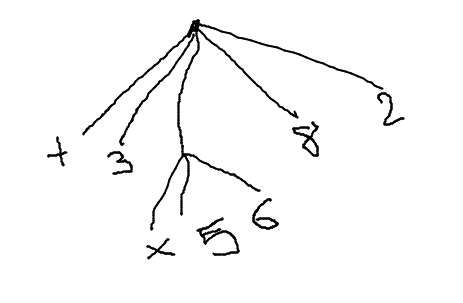
\includegraphics[scale=0.5]{assets/prefix_notation.jpg}
\end{center}
where each pair of parenthesis means a new combination = subtree. Recall when we think about languages we care about means of combination.

\subsection{The elements of programming}
This section was taken from the book not the lecture videos. The building blocks of a computer program are:
\begin{enumerate}
    \item \texttt{expressions} - simple expression would be if you type a number. in Lisp you can add
          a \textbf{combination} expression such as (+ 1 10 22) where combinations are always in
          parenthesis.
          The execution of all (simple or complex) expression is the same: The interpreter always operates
          in the same basic cycle: it reads an expression from the terminal, evaluates the expression,
          and prints the result. is mode of operation is oen
          expressed by saying that the interpreter runs in a \textbf{read-eval-print} loop.
    \item \texttt{naming and environment} - a critical aspect of a programming language is the means
          it provides for using names to refer to computational objects. We say that the name
          identifies a variable whose value is the object.
          in general, computational objects may have very complex structures, and it would be extremely
          inconvenient to have to remember and repeat their details each time we want to use them.
          Indeed, complex programs are constructed
          by building, step by step, computational objects of increasing complexity.
          it should be clear that the possibility of associating values with symbols and later
          retrieving them means that the
          interpreter must maintain some sort of memory that keeps track of the name-object pairs.
          This memory is called the \textbf{environment} (more precisely the \textbf{global environment},
          since we will see later that a computation may involve a number
    \item \texttt{evaluating combination} - how does the computer execute your lines of code.
          To evaluate a combination, do the following:
    \item evaluate the subexpressions of the combination.
    \item apply the procedure that is the value of the leftmost subexpression (the operator) to the
          arguments that are the values of the other subexpressions (the operands).
          Even this simple rule illustrates some important points about processes
          in general. First, observe that the first step dictates that in order to accomplish the
          evaluation process
          for a combination we must first perform the evaluation process on each element of the
          combination. Thus, the evaluation rule is recursive in nature; that is, it includes, as
          one of its steps, the need to invoke the rule itself. The recursion stops when the
          combination the computer need to compute contains only of \textbf{primitive} objects.
    \item \texttt{procedures/functions} - procedure definitions are much
          more powerful abstraction technique by which a compound operation can be given a name and
          then referred to as a unit.
          \\ Procedures/functions \textbf{wrap} ideas.
\end{enumerate}

\subsection{Procedures as black-box abstractions}
A consequence of having procedures/function is that we are able to modularize our code.
\textbf{Most importantly we can give these procedures a name as similarly as black-magic and
    witchcraft the true power comes when you have the names of your spells.} \texttt{sqrt} is our
first example of a process defined by a set of mutually defined
procedures. Observe that the problem of computing square roots breaks up naturally into a number of
subproblems: how to tell whether a guess is good enough, how to improve a guess, and so on. Each of these tasks is
accomplished by a separate procedure.
\begin{center}
    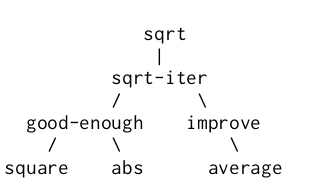
\includegraphics[scale = 0.5]{assets/sqrt.png}
\end{center}
The entire sqrt program can be viewed as a cluster of procedures (shown in Figure above) that mirrors
the decomposition of the problem into subproblems.
\begin{center}
    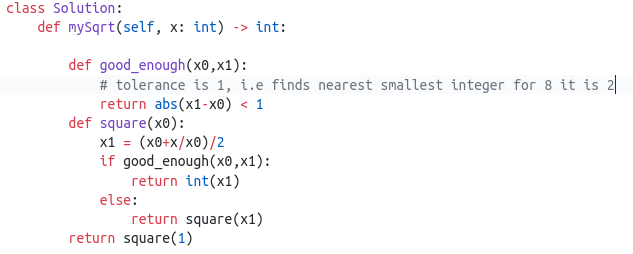
\includegraphics[scale = 0.5]{assets/sqrt_example.png}
\end{center}
The importance of this decomposition strategy is not simply that one is dividing the program
into parts. After all, we could take any large program and divide it into parts—the first ten lines,
the next ten lines, the next ten lines, and so on. Rather, it is crucial that each procedure
accomplishes an identifiable task that can be used as a module in defining other procedures.
For example, when we define the good-enough? procedure in terms of square , we are able to regard
the square procedure as a "black box.” We are not at that moment concerned with how the procedure
computes its result, only with the fact that it computes the square. Thee details of how the square is
computed can be suppressed,
to be considered at a later time. indeed, as far as the good-enough? procedure is concerned,
square is not quite a procedure but rather an abstraction of a procedure, a so-called
\textbf{procedural abstraction}. At this level of abstraction, any procedure that computes the square
is equally good.
A user should not need to know how the procedure is implemented in order to use it. \newline
There is another concept used in the above example. The nesting of definitions, called
\textbf{block structure}, is basically the right solution to the simplest name-packaging problem.
If we put the \texttt{good-enough} and \texttt{square} (better be named square-guess) outside the
\texttt{mySqrt} function, then they would only clutter up their minds.The only procedure that is
important to users of \texttt{sqrt} is \texttt{mySqrt}. They may not define any other procedure
called \texttt{good-enough} as part of another program to work together with the square-root program,
because sqrt needs it. Thee problem is especially severe in the construction of large systems by many
separate programmers. For example, in the construction of a large library of numerical procedures,
many numerical functions are computed as successive approximations and thus might have procedures
named good-enough? and improve as auxiliary procedures. We would like to localize the subprocedures,
Hiding them inside sqrt so that sqrt could coexist with other successive approximations, each having
its own private good-enough? procedure. To make this possible, we allow a procedure to have internal
definitions that are local to that procedure.

\subsection{Summary}
The three big topics of the course are:
\begin{itemize}
    \item Black-box abstraction
    \item Conventional interfaces
    \item Meta-linguistic abstraction
\end{itemize}
Our goal in this course is to explore computation, especially how thinking about computation can
serve as a tool for understanding and controlling complexity in large systems. We want to capture
descriptions of \textbf{computational processes}. We will see that to describe processes, we need
a language appropriate for capturing the essential elements of processes. This means we will need
fundamental primitives (or atomic elements of the language), means of combination (ways of constructing
more complex things from simpler ones) and means of abstraction (ways of treating complex things as
primitives so that we can continue this process).
\begin{example}
    Remember when thinking about languages we care about:
    \begin{itemize}
        \item primitive elements - procedures such as $+ - * /$, data such as 23, 3.14.
        \item means of combination - procedures such as  composition $()$, conditional statements \texttt{if else}.
        \item means of abstraction - procedures such as \texttt{def}, equivalently giving names
              to procedures and variables (in lisp keyword define is used to declare variables).
    \end{itemize}
\end{example}

\section{Lecture 1B: Procedures and Processes; Substitution Model}
The job of a programmer is to design processes to accomplish a particular goal. The way which he/she
does it is by constructing "spells" which are constructed out of procedures and expressions.
In order to do tat effectively, the programmer needs to understand how his procedures maps to the
execution of them by the machine. We would consider a \textbf{semi}-formal model which would
describe how procedures and expressions are ran by the machine. The model considered is
\textbf{the substitution} model which is just an approximation of how machine work.
Like all models (engineering, mathematical, statistical, computational) they just approximate reality.
The kinds of expressions we have are:
\begin{itemize}
    \item numbers
    \item symbols
    \item $\lambda$-expressions
    \item definitions
    \item conditionals
    \item combinations
\end{itemize}

\subsection{How does computer execute code?}
We describe the simplest model which could describe how computers execute/evaluate code - \textbf{the substitution rule}. To evaluate an application (using substitution rule):
\begin{enumerate}
    \item evaluate the operator to get procedure
    \item evaluate the operands to get arguments
    \item apply the procedure to the arguments by copying the body of the procedure, substituting
          the arguments supplied for the initial parameters of the procedure.
    \item evaluate new body (recursively until reach only primitive operators and operands)
\end{enumerate}
The key of understanding complicated things is to know what not to look at and think about. For
example if we compute square sum of 3 and 4 we can assume addition and multiplication are primitive
operators and need not to "unfold" them. You need to decide which details to ignore. NB the substitution rule is not a good description of how the machine works - but it is good for the next few lectures.
\begin{proposition}
    The substitution model gives a mechanical way to describe approximately how processes evolve when
    procedures are evaluated by the machine. it is only the first of these
    models—a way to get started thinking formally about the evaluation process. Later we will present
    a sequence of increasingly elaborate models of how interpreters work, culminating with a complete
    implementation of an interpreter and compiler.
\end{proposition}
The substitution model can be taken as a model that determines the
"meaning” of procedure application, insofar as the procedures in this
chapter are concerned. However, there are two points that should be
stressed:
\begin{itemize}
    \item The purpose of the substitution is to help us think about procedure \\
          application, not to provide a description of how the interpreter really works.
          Typical interpreters do not evaluate procedure applications by manipulating the text of a
          procedure to
          substitute values for the formal parameters. in practice, the "substitution” is
          accomplished by using a local environment for the formal parameters.
    \item The substitution model is only the first of these
          models—a way to get started thinking formally about the evaluation process.
          in general, when modeling phenomena in science and engineering, we begin with simplified,
          incomplete models. As we examine things in greater detail, these simple models become inadequate and must be
          replaced by more refined models. \\
          The substitution model is no exception
\end{itemize}

\subsection{Procedures and the Processes they generate. iterative vs Recursive processes}
We have now considered the elements of programming: We have used primitive arithmetic \\
operations, we have combined these operations, and we have abstracted these composite operations by
defining them as compound procedures. But that is not enough to enable us to say that we know how to program. Our situation is analogous to that of someone who has
learned the rules for how the pieces move in chess but knows nothing of typical openings, tactics,
or strategy. Like the novice chess player, we don't yet know the common patterns of usage in the
domain. We lack the knowledge of which moves are worth making (which procedures are worth defining).
 We lack the experience to predict the consequences of making a move (executing a procedure).
 In programming we are planning the course of action to be taken by a process and
we control the process by means of a program. To become experts, we must learn to visualize the
processes generated by
various types of procedures.
Only after we have developed such a skill can we learn to reliably construct programs that exhibit
the desired behavior.
\begin{definition}
    A procedure can be regarded as a pattern for the local evolution of a process, and we classified,
    reasoned about, and performed simple algorithmic analyses of some common patterns for processes
    as embodied in procedures.
\end{definition}
\begin{proposition}
    A procedure is a pattern for the local evolution of a computational process.it specifies how each
    stage of the process is built upon the previous stage.
\end{proposition}
We would like to be able to make statements about the overall, or \textbf{global}, behavior of a
process whose local evolution has been specified
by a procedure. There are two main types of processes computers execute:
\begin{itemize}
    \item iterative
    \item Recursive
\end{itemize}
When we consider the "shapes” of the two processes, we
find that they evolve quite differently. in recursion the expansion occurs as the process builds up a
chain of deferred operations (in computing factorial case, a chain of multiplications).
The contraction occurs as the operations are actually performed. Carrying out this process requires
that the interpreter keep track of the operations to be performed later on.By contrast, the second process does not grow and shrink. At each step, all we need to keep track of, for any n, are the current values of the variables product, counter, and max-count .\newline The contrast between the two processes can be seen in another way way. in the iterative case, the program variables provide a complete description of the state of the process at any point. if we stopped the computation between steps, all we would need to do to resume the computation is to supply the interpreter with the values of the three program variables. Not so with the recursive process. in this case there is some additional "hidden” information, maintained by the interpreter and not contained in the program variables, which indicates "where the process is” in negotiating the chain of deferred operations. The longer the chain,
the more information must be maintained.
\subsection{Order of growth}
Processes can differ considerably in the rates at which they consume computational resources. One
convenient way to describe this difference is to use the notion of order of growth to obtain a gross
measure of the resources required by a process as the inputs become larger.
\begin{definition}
    We say that R(n) has order of growth $\Theta(f(n))$, written $R(n) = \Theta(f(n))$
    (pronounced "theta of $f(n)$”), if there are positive constants $k_1$ and $k_2$ independent of $n$
    such that $k_1 f(n) \leq R(n) \leq k_2 f(n)$ for any sufficiently large value of $n$. (in other words,
    for large $n$, the value $R(n)$ is sandwiched between $k_1 f(n)$ and $k_2 f (n)$.)
\end{definition}
Orders of growth provide only a crude description of the behavior
of a process. For example, a process requiring $n^2$ steps and a process
requiring 1000$n^2$ steps and a process requiring $3n^2 + 10n + 17$ steps all have $\Theta(f(n))$ order of growth.

\subsection{Greatest common divisor}
The greatest common divisor (GCD) of two integers a and b is defined to
be the largest integer that divides both a and b with no remainder. For
example, the (GCD) of 16 and 28 is 4.   The idea of the algorithm is based on the observation that,
if r is the remainder when a is divided by b, then the common divisors of a and b are precisely
the same as the common divisors of b and r .
\begin{center}
    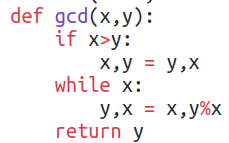
\includegraphics[scale = 0.4]{assets/gcd.png}
\end{center}
e fact that the number of steps required by Euclid's Algorithm
has logarithmic growth bears an interesting relation to the Fibonacci
numbers:
\begin{theorem}
    Lamé's Theorem: if Euclid's Algorithm requires $k$ steps to
    compute the(GCD) of some pair, then the smaller number in
    the pair must be greater than or equal to the $k$-th Fibonacci
    number.
\end{theorem}
We can use this theorem to get an order-of-growth estimate for Euclid's
Algorithm. Let n be the smaller of the two inputs to the procedure.
if the process takes $k$ steps, then we must have $n \geq Fib(k) \approx \phi^k / 5$. therefore
the number of steps $k$ grows as the logarithm (to the base $\phi$) of $n$. Hence, the order of
growth is $\Theta(log n)$.

\subsection{Example: Testing for Primalily}
This section describes two methods for checking the primality of an integer $\sqrt{n}$, one with
order of growth $\Theta(n)$, and a "probabilistic” algorithm with order of growth $\Theta(log n)$.
The first one is obvious, the second one is called the Fermat test.

\begin{definition}
    Fermat's Little Theorem: if n is a prime number and a
    is any positive integer less than n, then a raised to the n-th
    power is congruent to a modulo n.
\end{definition}

if n is not prime, then, in general, most of the numbers $a < n$ will
not satisfy the above relation. This leads to the following algorithm for testing primally:
Given a number n, pick a random number $a < n$ and compute the remainder of a n modulo n. if the
result is not equal to a, then n is certainly not prime. if it is a, then chances are good that n is
prime. Now pick another random number a and test it with the same
method. if it also satisfies the equation, then we can be even more confident that n is prime.
By trying more and more values of a, we can
increase our confidence in the result. This algorithm is known as the
Fermat test. if n ever fails the Fermat test, we can be certain that n is not prime. But the fact
that n passes the test, while an extremely strong indication, is still not a guarantee that n is prime.
What we would like to say is that for any number n, if we perform the test enough times and find that
n always passes the test, then the probability of error in our primality test can be made as small
as we like.

\section{Lecture 2A: Higher-order Procedures}
Note that the terms \textbf{procedures} and \textbf{functions} are used interchangeably. We have seen
that procedures are, in effect, abstractions that describe compound operations on numbers independent
of the particular numbers. Yet even in numerical processing we will be severely limited in our ability
to create abstractions if we are restricted to procedures whose parameters must be numbers. One of
the things we should demand from a powerful programming language is the ability to build abstractions b
y assigning names to common patterns and then to work in terms of the abstractions directly.
Procedures provide this ability. This is why all but the most primitive programming
languages include mechanisms for defining procedures. Often the same programming pattern will be
used with a number of different procedures. To express such patterns as concepts, we will need
to construct procedures that can accept procedures as arguments or return procedures as values.
Procedures that manipulate procedures are called higher-order procedures.
\begin{definition}
    A function is called Higher Order Function if it contains other functions as a parameter or
    returns a function as an output i.e, the functions that operate with another function are
    known as Higher order Functions.
\end{definition}

\begin{center}
    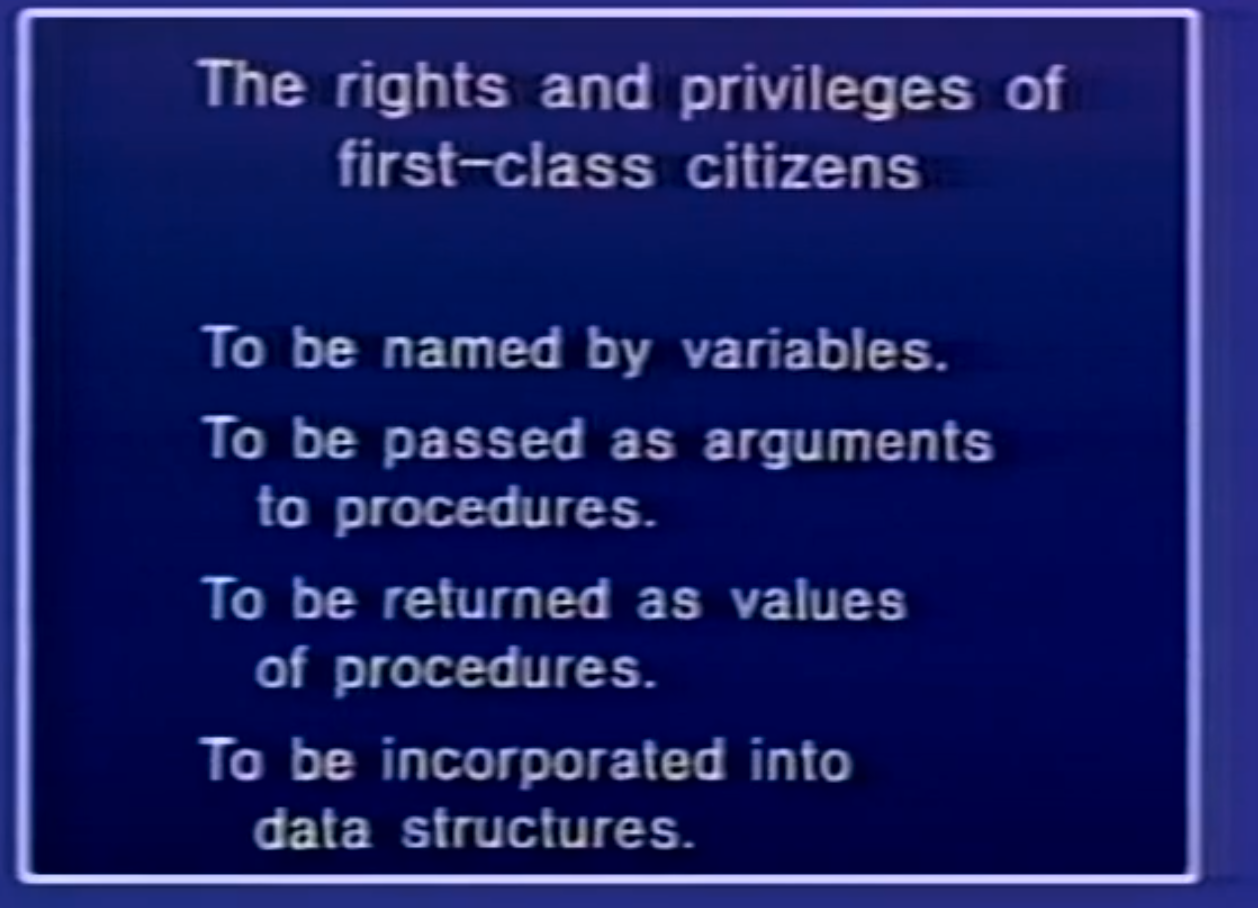
\includegraphics[scale=0.2]{assets/first-class-citizens.png}
\end{center}
Higher-order procedures can serve as powerful abstraction mechanisms, vastly increasing the \\
expressive power of our language. it is worth knowing that this higher order function
is applicable for functions and methods as well that takes functions as a parameter or
returns a function as a result. Python too supports the concepts of higher order functions.
Functions/Procedures are first-class citizens in Python/Lisp. They are no different than numbers.
Passing function to other functions is the way they talk with each other.
This is very important because: whenever trying to make complicated systems and
understand them, its crucial to divide the things up into as many pieces as I can -
each of which I can understand separately. I would like to  understand the way of
adding things up independently of what it is i'm adding up so I can use that having
debugged it once/ understand it ONCE. For example the function
\texttt{sum} should be able to add different inputs: consecutive integers,
even integers, odd integers, floats, strings etc. Any time you encounter things which seem
identical, you'd need to come up with an abstraction to cover them. \newline
As programmers, we should be alert to opportunities to identify the
underlying abstractions in our programs and to build upon them and
generalize them to create more powerful abstractions. This is not to
say that one should always write programs in the most abstract way
possible; expert programmers know how to choose the level of abstraction appropriate to their task.
But it is important to be able to think in
terms of these abstractions, so that we can be ready to apply them in
new contexts. The significance of higher-order procedures is that they
enable us to represent these abstractions explicitly as elements in our
programming language, so that they can be handled just like other computational elements. \newline
in general, programming languages impose restrictions on the ways
in which computational elements can be manipulated. Elements with
the fewest restrictions are said to have first-class status. Some of the
"rights and privileges” of first-class elements are:
\begin{itemize}
    \item They may be named by variables.
    \item They may be passed as arguments to procedures.
    \item They may be returned as the results of procedures.
    \item They may be included in data structures
\end{itemize}
\section{Lecture Lecture 2B: Compound Data}

\subsection{Building Abstractions with Data}
We saw how to use primitive data (numbers) and primitive operations (arithmetic operations),
how to combine procedures to form compound procedures \\ \textbf{(means of combination)} through
composition, conditionals, and the use of parameters, and how to abstract procedures by using define
\textbf{(means of abstraction)}.
\begin{proposition}
    The crucial idea is that when we are building things we divorce the tasks of building things
    from the task of implementing the task. The key is to build big systems in layers, isolating
    the details at the lower layers.
\end{proposition}
in this chapter we are going to look at more complex data. We will see how to compound data (same as
we saw how to compound procedures/functions).\newline
Why do we want compound data in a programming language? For the same reasons that we want compound
procedures: to elevate the conceptual level at which we can design our programs, to increase the
modularity of our designs, and to enhance the expressive power of our
language. The use of compound data leads to a real increase in the expressive power of our \\
programming language.
\begin{remark}
    The strategy of \textbf{wishful} thinking is extremely powerful design strategy when building complex computational systems. Just image imagine what you want to have that you already have it and start think what it can do. Usually you use wishful thinking to assume that you have a particular data object/procedure, that you still don't have.
\end{remark}
As with compound procedures, the main issue to be addressed is that of abstraction as a \\
technique for coping with complexity, and we will see how data abstraction enables us to erect suitable
abstraction barriers between different parts of a program.\newline
Consider the task of designing a system to perform arithmetic with rational numbers.
We could imagine an operation add-rat that takes two rational numbers and produces their sum.
in terms of simple data, a rational number can be thought of as two integers: a numerator and a denominator.
us, we could design a program in which each rational number would be represented by two integers
(a numerator and a denominator) and where add-rat would be implemented by two procedures (one producing
the numerator of the sum and one producing the denominator).denominator and where add-rat would be
implemented by two procedures (one producing the numerator of the sum and one producing the denominator).
The key to forming compound data is that a programming language should provide some kind of "glue” so that
data objects can be combined to form more complex data objects. There are many possible kinds of glue.
indeed, we will discover how to form compound data using no special "data” operations at all, only procedures.
This will further blur the distinction between "procedure” and "data,” which was already becoming tenuous toward
the end of chapter 1. We will also explore some conventional techniques for representing sequences
and trees.
ne key idea in dealing with compound data is the notion of \textbf{closure} —
that the glue we use for combining data objects should allow
us to combine not only primitive data objects, but compound data objects as well. Another key idea
is that compound data objects can serve
as \textbf{conventional interfaces} for combining program modules in mix-and-match ways.
\begin{definition}
    Data abstraction is a methodology that enables us to isolate how a compound data object is used
    from the details of how it is constructed from more primitive data objects.
\end{definition}
The basic idea of data abstraction is to structure the programs that are to use compound data objects
so that they operate on "abstract data". That is, our programs should use data in such a way as to make no assumptions about the data that are not strictly necessary for performing the task at hand. At the same time, a "concrete” data representation is defined independent of the programs that use the data. The interface between these two parts of our system will be a set of procedures, called \textbf{selectors and constructors}, that implement the abstract data in terms of the concrete representation.
\subsubsection{Abstraction Barriers}
We defined the rational-number operations in terms of a constructor make-rat and selectors numer and denom.
in general, the underlying idea of data abstraction is to identify for each type of data object a basic set of operations in terms of which all manipulations of data objects of that type will be expressed, and then to use only those operations in manipulating the data. We can envision the structure of the rational-number system as
shown in the below figure.
\begin{center}
    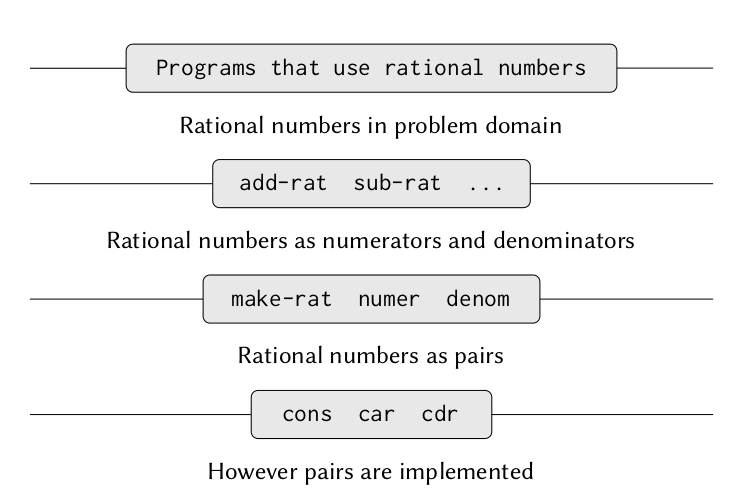
\includegraphics[scale=0.2]{assets/data_abstraction.png}
\end{center}
The horizontal lines represent abstraction barriers that isolate different "levels” of the system.
At each level, the barrier separates the programs (above) that use the data abstraction from the
programs (below) that implement the data abstraction. \textbf{Note how we have separated the use of
data objects to the representation of the objects}. This programming methodology is called
\textbf{data abstraction}. This simple idea has many advantages. One advantage is that it makes
programs much easier to maintain and to modify. Any complex data structure can be represented in a
variety of ways with the primitive data structures provided by a programming language. Of course,
the choice of representation influences the programs that operate on it; thus, if the representation
were to be changed at some later time, all such programs might have to be modified accordingly. \newline
Constraining the dependence on the representation to a few interface procedures helps us design
programs as well as modify them, because it allows us to maintain the flexibility to consider alternate
implementations. To continue with our simple example, suppose we
are designing a rational-number package and we can't decide initially whether to perform the gcd at
construction time or at selection time. Te data-abstraction methodology gives us a way to defer that
decision without losing the ability to make progress on the rest of the system. indeed the powers of
such system design is the independent layers of it. To sum up, the two real powers of data abstraction
are:
\begin{itemize}
    \item Constructing layers when building a complex system. These layers are independent of each other and is less prone to break everything.
    \item Giving names to the newly compounded data (such as rational numbers). This allows us to encapsulate and materialize ideas from our minds. \textbf{Programming is like black magic or witchcraft - the true power of your spells comes when you have names for them}.
\end{itemize}
\subsection{What is Meant by Data?}
We began the rational-number implementation in before by implementing the rational-number operations add-rat, sub-rat, and so on in terms of three unspecified procedures: make-rat, numer, and denom. At that point, we could think of the operations as being defined in terms of data objects—numerators, denominators, and rational numbers—whose behavior was specified by the later three procedures. But exactly what is meant by data ? it is not enough to say "whatever is implemented by the given selectors and constructors.” Clearly, not every arbitrary set of three procedures can serve as an appropriate basis for the rational-number implementation. We need to guarantee that, if we construct a rational number x from a pair of integers n and d , then extracting the numer and the denom of x and dividing them should yield the same result as dividing n by d.
\begin{example}
    Say we ask George to create for us an object rational-number which support addition, multiplication and
    the gcd of numerator and denominator. He cannot just go and write the constructor and three procedures and give us that.
    The contract is that these procedures should do what real rational numbers do.
    That is the object George creates should be valid representation of the mathematical notion of rational numbers.
\end{example}

\begin{definition}
    in general, we can think of data as defined by some collection of selectors and constructors, together with specified conditions that these
    procedures must fulfill in order to be a valid representation
\end{definition}
in Lips we construct a rational number using this:
\begin{center}
    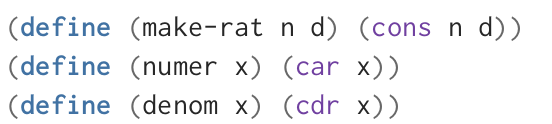
\includegraphics[scale = 0.3]{assets/rational_number_constr.png}
\end{center}
\texttt{cons} is the constructor which builds a \texttt{pair} object in Lips. \newline
\texttt{car} is a method that gets the first element of the pair\newline
\texttt{car} is a method that gets the first element of the pair\newline
We never actually define what a pair is, only that the language
supplied procedures \texttt{cons}, \texttt{car},and \texttt{cdr} for operating on pairs.
But the only thing we need to know about these three operations is that if we glue two objects
together using cons we can retrieve the objects using \texttt{car} and \texttt{cdr}.
That is, the operations satisfy the condition that, for any objects x and y , if z is (\texttt{cons} x y)
then (\texttt{car} z) is x and (\texttt{cdr} z) is y. \newline
The layers of abstraction we have are: rational number - pair - thin air.
Below is an implementation of pair object using only procedures, i.e there is nothing below pair objects!
\begin{center}
    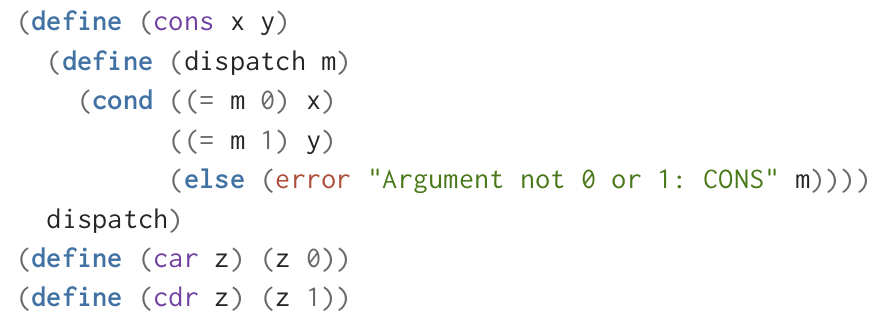
\includegraphics[scale = 0.3]{assets/thin-air.png}
\end{center}
We have built all three methods \texttt{cons}, \texttt{car}, \texttt{cdr}
using thin air, hence we are in the business of creating pair objects. Therefore, this
procedural implementation of pairs is a valid implementation,
and if we access pairs using only \texttt{cons}, \texttt{car}, \texttt{cdr}
we cannot distinguish this implementation from one that uses "real" data structures.\newline
\textbf{Question.} When calling the \texttt{cons} method multiple times how does it
know to differentiate the different calls
with different arguments $x, y$.
\textit{Procedures are not just the act of doing something, they are conceptual entities - objects
    and if i
    build a cons 2 45 and cons 3 1 they would be different. Procedures are objects. This is a
    different way of
    thinking about procedures - they don't just do things but they are objects. When you have
    procedures which
    return procedures you should think about these procedures as if they were objects.}
Another example is when you call \texttt{sqrt(5)} and \texttt{sqrt(9)}, then you are not
bothered that procedures can call different arguments and are different things. However in the
\texttt{cons} example above it returns another function which picks up arguments passed in cons.
These arguments return you a specified function $=$ object. This idea is behind using decorators in Python!
The point of exhibiting the procedural representation of pairs is not that our language works this way
(Scheme, and Lisp systems in general, implement pairs directly, for efficiency reasons) but that it
could work this way.
The procedural representation, although obscure, is a perfectly
adequate way to represent pairs, since it fulfills the only conditions that pairs need to fulfill.\\
This example also demonstrates that the ability to manipulate procedures as objects automatically
provides the ability to represent compound data.
This may seem a curiosity now, but procedural representations of data will play a central role in our
programming repertoire.
This style of programming is open called \textbf{message passing}.

\section{Lecture 3A: Henderson Escher Example}

\subsection{Hierarchical Data and the Closure Property}
As we have seen, pairs provide a primitive "glue” that we can use to construct compound data objects.
The figure below shows a standard way to visualize a pair—in this case, the pair formed by (cons 1 2).
in this representation, which is called box-and-pointer notation , each object is shown as a pointer
to a box. e box for a primitive object contains a representation of the object. For example,
the box for a number contains a numeral. the box for a pair is actually a double box,
the left part containing (a pointer to) the car of the pair and the right part containing the cdr.
\begin{center}
    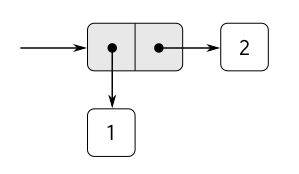
\includegraphics[scale = 0.5]{assets/box_pointer.png}
\end{center}
\begin{proposition}
    \texttt{cons} can be used to combine not only numbers but other pairs as well.
\end{proposition}
\begin{center}
    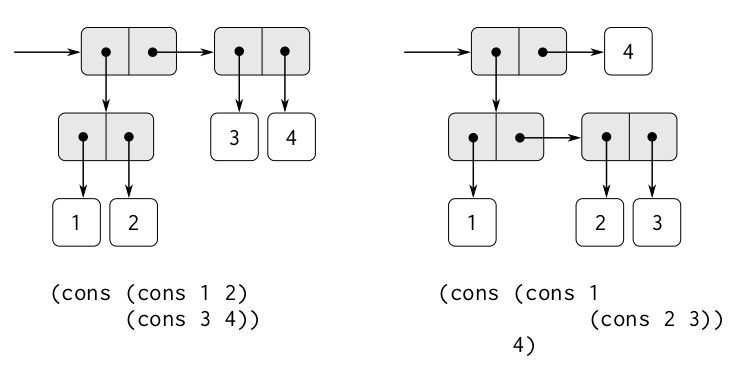
\includegraphics[scale = 0.25]{assets/cons_of_cons.png}
\end{center}
\begin{proposition}
    The ability to create pairs whose elements are pairs is the essence of list structure's
    importance as a representational tool.
    We refer to this ability as \textbf{the closure property} of \texttt{cons} .
\end{proposition}

\begin{proposition}
    The set of objects in Lisp/Python is closed under the operation of forming \\
    pairs/functions. That's the thing help us build complexities.
\end{proposition}
\textbf{in Python closures appear when you create functions to return other functions.} Decorators
are a form of closures in Python.
\begin{example}
    Arrays are closed under the operation of forming arrays. You can have array of arrays. When you
    are thinking about means of combination you should ask yourself is that thing a closure.
\end{example}
in general, an operation for combining data objects satisfies the closure property if the results of
combining things with that operation can themselves be combined using the same operation.\newline
Closure is the key to power in any means of combination because it permits us to create hierarchical
structures—structures made up of parts, which themselves are made up of parts, and so on.
\subsection{Representing Sequences in Lisp}
One of the useful structures we can build with pairs is a sequence an ordered collection of data objects.
There are, of course, many ways to represent sequences in terms of pairs. One particularly
straightforward representation is illustrated in figure, where the sequence 1, 2, 3, 4 is
represented as a chain of pairs. The car of each pair is the corresponding item in the chain,
and the cdr of the pair is the next pair in the chain.
\begin{center}
    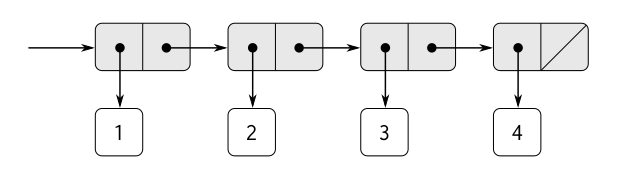
\includegraphics[scale = 0.25]{assets/lisp_list.png}
\end{center}
Such a sequence of pairs, formed by nested cons es, is called a list, and Scheme provides a primitive
called list to help in constructing lists. The above sequence could be produced by \texttt{(list 1 2 3 4)}.

\subsection{Example: A Picture Language}
in this section we discuss an example which would wrap up everything we have talked until now:
\begin{itemize}
    \item list structure
    \item issues of abstraction and representation
    \item how to capture commonality with higher order procedures
    \item meta-linguistic abstraction
\end{itemize}

\begin{remark}
    Meta-linguistic abstraction is the idea that one of the ways of tackling complexity in
    engineering design is to build a suitable powerful language.
\end{remark}
When you think about a language you think about what are the:
\begin{itemize}
    \item primitives
    \item means of combination - how to build bigger things
    \item means of abstraction - how do you take those bigger things that you've build and put
          black-boxes around them
\end{itemize}
The language we will talk about was made by Peter Hederson. This language is about making, describing,
drawing figures like that:
\begin{center}
    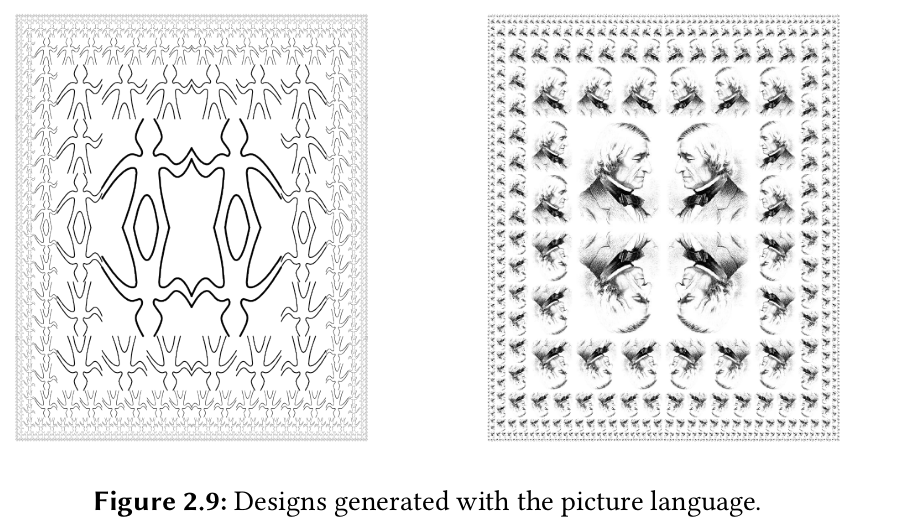
\includegraphics[scale = 0.5]{assets/pictures.png}
\end{center}
We will show that there is no difference between procedures and data. When we began our study of
programming in Section 1.1, we emphasized the importance of describing a language by focusing on the
language's
primitives, its means of combination, and its means of abstraction. We'll follow that framework here.
Part of the elegance of this picture language is that there is only one kind of element, called a painter.
A painter draws an image that is shifted and scaled to fit within a designated parallelogram-shaped frame.
\begin{center}
    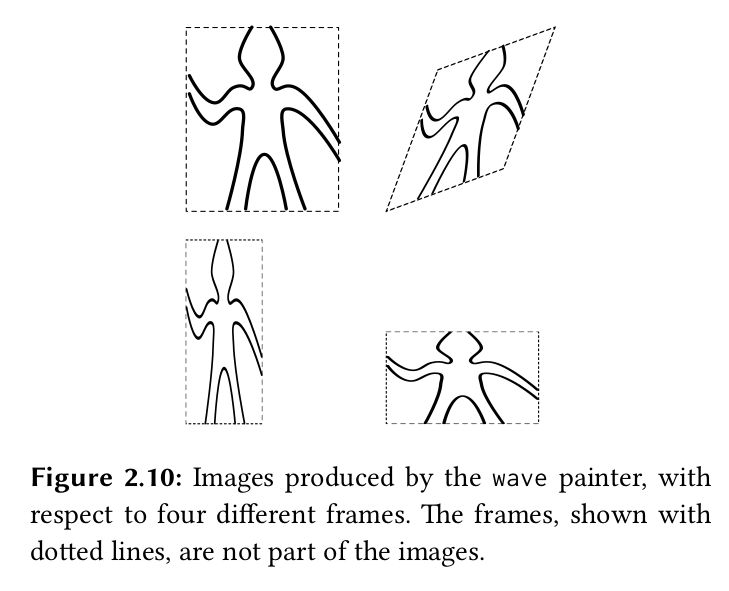
\includegraphics[scale = 0.5]{assets/painter_primitive.png}
\end{center}
To combine images, we use various operations that construct new
painters from given painters. For example, the \texttt{beside} operation takes two painters and
produces a new, compound painter that draws the first painter's image in the left half of the frame and
the second painter's image in the right half of the frame. Similarly, \texttt{below} takes two painters
and produces a compound painter that draws the first painter's image below the second painter's image.
Some operations transform a single painter to produce a new painter. For example, \texttt{flip-vert}
takes a painter and produces a painter that draws its image upside-down, and \texttt{flip-horiz}
produces a painter that draws the original painter's image left-to-right
reversed.
\begin{center}
    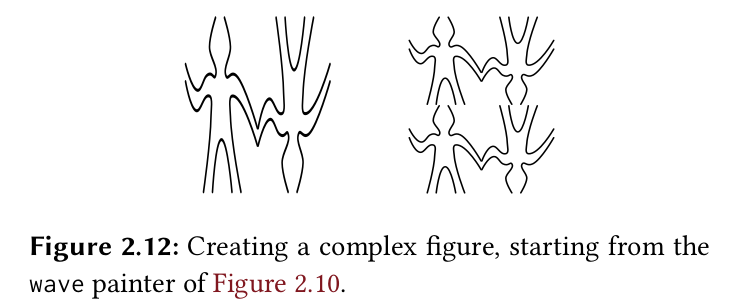
\includegraphics[scale = 0.5]{assets/complex_picture.png}
\end{center}
\begin{proposition}
    in building up a complex image in this manner we are exploiting the fact that painters are closed
    under the language's means of combination.
\end{proposition}
The above image can be produced by the following lines (assuming wave is the painter object).
\begin{lstlisting}
(define wave2 (beside wave (flip-vert wave)))
(define wave4 (below wave2 wave2))
\end{lstlisting}
The beside or below of two painters is itself a painter; therefore, we can use it as an element in
making more complex painters. As with building up list structure using cons, the closure of our data
under the means of combination is crucial to the ability to create complex structures while using only
a few operations. Notice how rapidly we have built up complexity, just in 15 seconds we got from a
single wave image to that thing in Figure 2.12. it is all because of the closure property.\newline
\textbf{Frames}\newline
Before we can show how to implement painters and their means of combination, we must first consider frames.
A frame can be described by three vectors—an origin vector and two edge vectors. The origin vector
specifies the offset of the frame's origin from some absolute origin in the plane, and the edge vectors
specify the offsets of the frame's corners from its origin. if the edges are perpendicular, the frame
will be rectangular. Otherwise the frame will be a more general parallelogram.
\begin{center}
    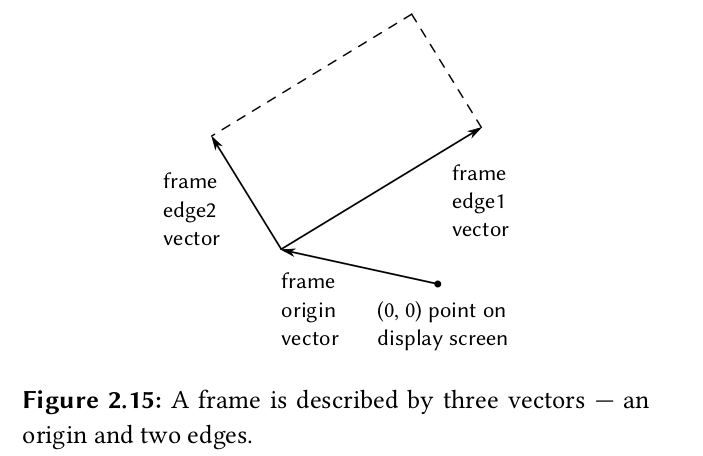
\includegraphics[scale = 0.5]{assets/frame.png}
\end{center}
We will use coordinates in the unit square $(0 \leq x, y \leq 1)$ to specify images. With each frame,
we associate a frame coordinate map , which
will be used to shift and scale images to fit the frame. The map trans-
forms the unit square into the frame by mapping the vector $v = (x , y)$
to the vector sum:
\begin{center}
    Origin(Frame) + x · Edge 1 (Frame) + y · Edge 2 (Frame).
\end{center}
\textbf{Painters}\newline
A painter is represented as a procedure that, given a frame as argument,
draws a particular image shited and scaled to fit the frame. That is to
say, if p is a painter and f is a frame, then we produce p 's image in f by
calling p with f as argument. The details of how primitive painters are implemented depend on the
particular characteristics of the graphics system and the type of image to be drawn. For instance,
suppose we have a procedure draw-line that draws a line on the screen between two specified points.
Then we can create painters for line drawings, such as the wave painter in Figure 2.10, from lists
of line segments as follows:
\begin{lstlisting}
(define (segments->painter segment-list)
(lambda (frame)
(for-each
(lambda (segment)
(draw-line
((frame-coord-map frame)
(start-segment segment))
((frame-coord-map frame)
(end-segment segment))))
segment-list)))
\end{lstlisting}
The segments are given using coordinates with respect to the unit square.
For each segment in the list, the painter transforms the segment end-
points with the frame coordinate map and draws a line between the
transformed points. Representing painters as procedures erects a powerful abstraction
barrier in the picture language. We can create and intermix all sorts of
primitive painters, based on a variety of graphics capabilities. The details of their implementation
do not matter. Any procedure can serve as a painter, provided that it takes a frame as argument and
draws something scaled to fit the frame.

\textbf{Levels of language for robust design}\newline
The picture language exercises some of the critical ideas we've introduced about abstraction with
procedures and data. The fundamental data abstractions, painters, are implemented using procedural
representations, which enables the language to handle different basic drawing capabilities in a
uniform way. The means of combination satisfy the closure property, which permits us to easily
build up complex designs.
Finally, all the tools for abstracting procedures are available to us for
abstracting means of combination for painters.
\begin{remark}
    The picture language shows the notion of nicely \textbf{embedding} a language inside language.
    All the power of of this language like Lisp of the surrounding language is still accessible to
    you. This is similar to the way the Python is written in C!
\end{remark}
We have also obtained a glimpse of another crucial idea about languages and program design. This is
the approach of stratified design, the notion that a complex system should be structured as a
sequence of levels that are described using a sequence of languages. Each level is constructed by
combining parts that are regarded as primitive at that level, and the parts constructed at each level
are used as primitives at the next level. The language used at each level of a stratified design
has primitives, means of combination, and means of abstraction appropriate
to that level of detail.

Stratified design pervades the engineering of complex systems. For example, in computer engineering,
resistors and transistors are combined (and described using a language of analog circuits) to produce
parts such as and-gates and or-gates, which form the primitives of a language for digital-circuit design.
These parts are combined to build processors, bus structures, and memory systems, which are in turn
combined to form computers, using languages appropriate to computer architecture. Computers are
combined to form distributed systems, using
languages appropriate for describing network interconnections, and so
on.

Stratified design helps make programs robust , that is, it makes it
likely that small changes in a specification will require correspondingly
small changes in the program.

Stratified design gives you levels of languages rather than a strict hierarchy. Not only that but when you have levels of languages you have given yourself different vocabulary for talking about the design of level of language you are. The real power of Lisp and the fact that the means of combinations are procedures which are closed under means of combination is that you can create new languages, not just programs! it is basically the power of every OOP language! Being able to create your own Objects, level of abstraction and these object can talk with each other in their own language.

\subsection{Stratified Design over Layered Design}
Some notes on the Medium article about \href{Stratified Design}{https://medium.com/clean-code-development/stratified-design-over-layered-design-125727c7e15}.
\begin{definition}
    A layered software design is one in which when the call relationships among different modules are
    represented graphically, it would result in a tree-like diagram with clear layering. in the
    layered design, the modules are arranged in the hierarchy of layers. in such design, a module can only invoke functions of the modules in the layer immediately below it. The higher layer module can be considered similar to management who can invoke lower layer module to get a certain task done.
\end{definition}
Designing software with layers is common — and broken. it's broken for two reasons:
\begin{itemize}
    \item Layers suggest some form of abstraction; but layering very fundamentally is not about
          abstraction.
    \item Layering relies on functional dependencies which are hard to test and make software
          difficult to understand and evolve.
\end{itemize}
The next two figures show a layered design (commonly used in practice).
\begin{center}
    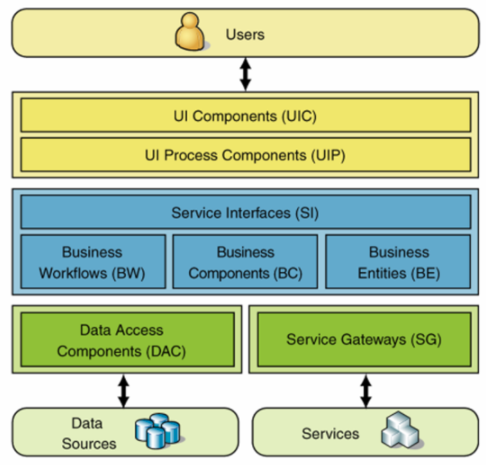
\includegraphics[scale = 0.3]{assets/layered_design.png}
\end{center}

\begin{center}
    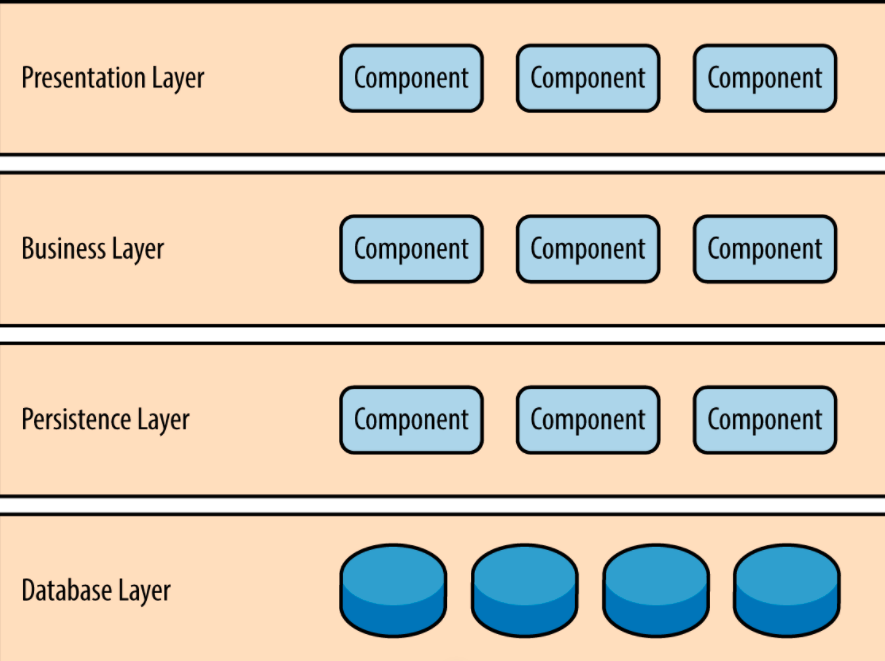
\includegraphics[scale = 0.3]{assets/layered_design_two.png}
\end{center}
in layered design there is no actual \textbf{abstraction}.Doing some Ui stuff is not on a higher level of abstraction than doing some business stuff, which is not on a higher level of abstraction than doing data access stuff. Ui and business and data access are just different stuff on the same level of abstraction. Asking your mom for some bacon and toast and butter and salad is not on a higher level of abstraction than putting these ingredients together in a sandwich. But a recipe is on a different level of abstraction!
\begin{center}
    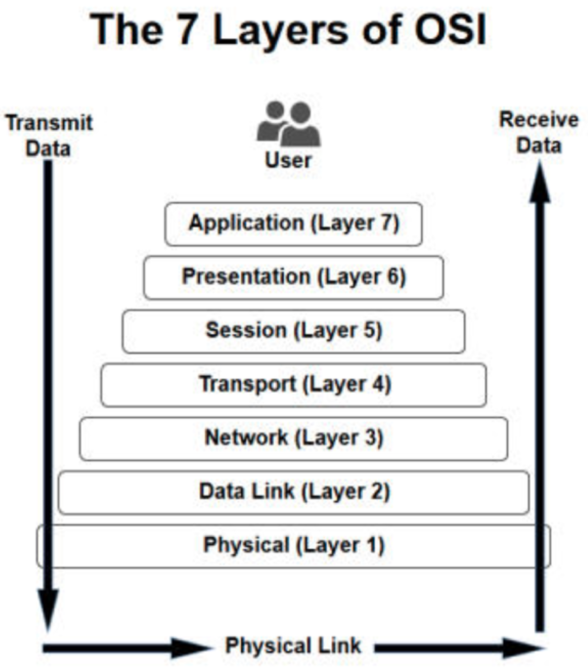
\includegraphics[scale = 0.3]{assets/osi_layers.png}
\end{center}
The Open Systems interconnection model (OSi model) is a conceptual model that describes the universal
standard of communication functions of a telecommunication system or computing system, without any
regard to the system's underlying internal technology and specific protocol suites.
Each layer in the OSi model has its own well-defined functions, and the functions of
each layer communicate and interact with the layers immediately above and below it, unless
the layer does not have layers below or above. in either case, each layer of the OSi model
has its own well-defined functions that describe the basic applications for communication of all
communication protocols. it's extraordinarily deplorable that the term "layer" got used in both models. This has caused much
confusion. And it has added value to the layered software design pattern which it does not deserve. \newline
We will use the term \textbf{strata} to mean the seconde beetter types of layers. This terminology
is taken from the MiT Lisp \href{paper}{https://dspace.mit.edu/bitstream/handle/1721.1/6064/AiM-986.pdf}.
"The 7 Layers of OSi" then become "The 7 Strata of OSi".

To make the distinction between layers and strata more tangible consider the example:
\begin{example}
    A user enters a one line text through the console and the program determines \newline
    the number of words in the text. But not all words count! Some stop words defined in the file \textit{"stopwords.txt"} should be ignored.
\end{example}
That's a problem which can easily be solved with a layered software design:
\begin{center}
    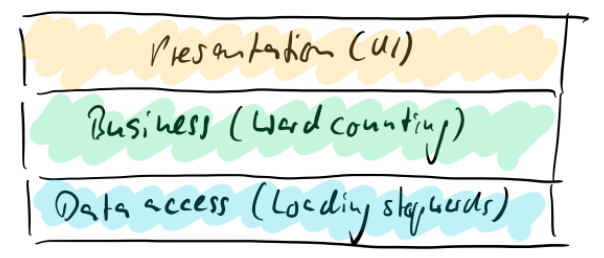
\includegraphics[scale = 0.3]{assets/example_layered.png}
\end{center}
The class dependencies might be simple:
\begin{center}
    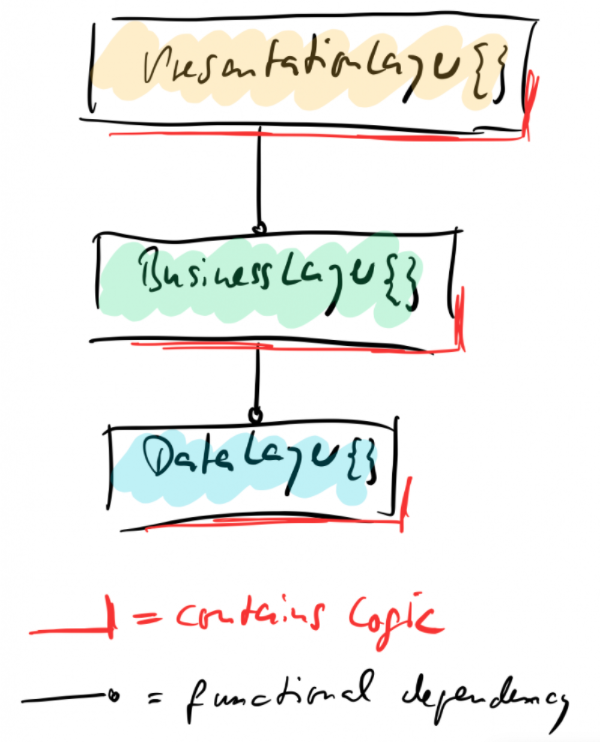
\includegraphics[scale = 0.3]{assets/tree_class.png}
\end{center}
But look closer! There are so many functions depending on each other, each containing logic calling logic in yet other functions:
\begin{center}
    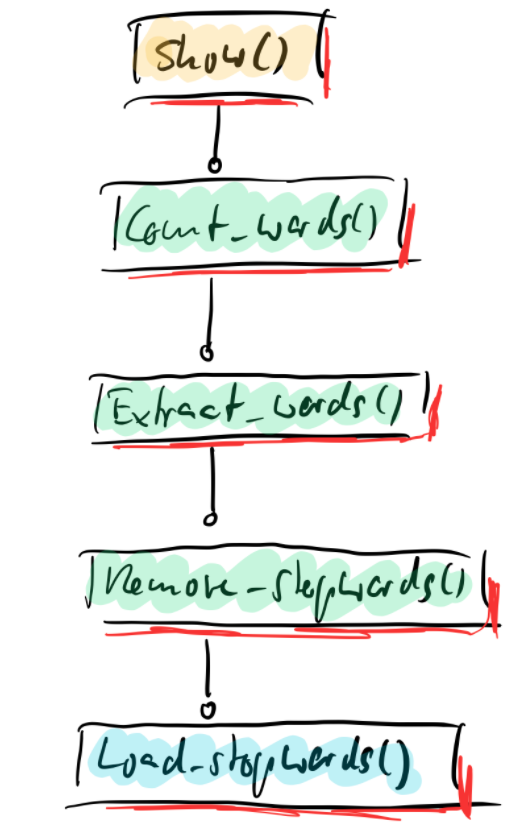
\includegraphics[scale = 0.3]{assets/tree_layered_example.png}
\end{center}
What needs to be done is not deeply nested but laid out sequentially. Check out the class design:

\begin{center}
    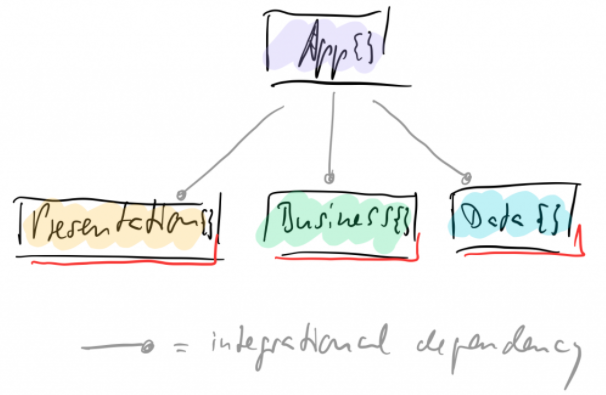
\includegraphics[scale = 0.3]{assets/level_hierarchy.png}
\end{center}
it makes even more clear how independent the functional aspects of the solutions are. Only \texttt{App()} knows the workhorse classes – but \texttt{App()} does not contain any logic. it's only there to integrate the parts into a whole. But that's a very important task! it's a responsibility of its own to be separated from actually doing stuff like processing data or loading data. it has this functional tree:
\begin{center}
    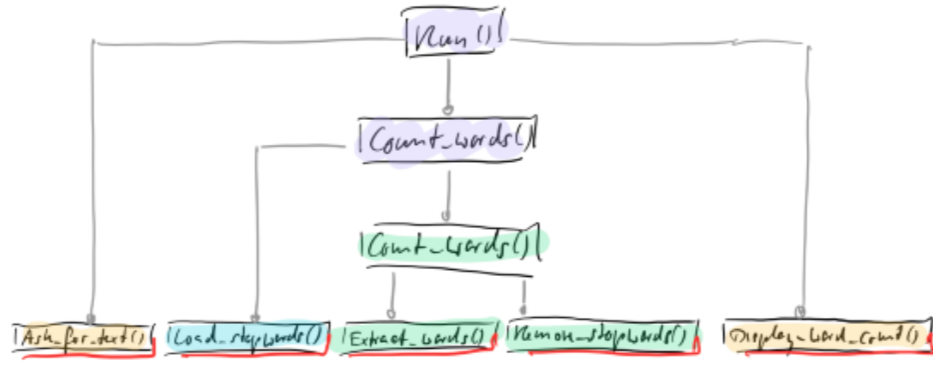
\includegraphics[scale = 0.3]{assets/strata_tree.png}
\end{center}
\begin{proposition}
    The stratified design does not have as many functional dependencies as the layered design.
\end{proposition}
\begin{remark}
    The relationship between \texttt{App} and \texttt{Presentation} etc. is not functional!
    There is no logic in \texttt{App} which uses logic in \texttt{Presentation} etc.
    The relationship thus is purely \textbf{"integrational"}. indeed \texttt{Display\_Word\_Count()}
    is not a functional dependence of \texttt{Run()}.
\end{remark}

\begin{proposition}
    in stratified design all the logic only resides in the leafs of the call tree. Whereas in layered design it was in all layers.
\end{proposition}

\begin{definition}
    Define those functions with just logic in them and without any dependencies \textbf{operations}. The other ones without logic but with integrational dependencies are \textbf{integrations}.
\end{definition}
The overarching principle here is the integration Operation Segregation Principle (iOSP). it allows us to systematically reduce the complexity of large methods into much simpler ones. it becomes particularly important in Functional Programming and is often a staple of refactoring a code base for testing. it's a pattern we sometimes don't realise we are using but once we see it formalised we realise it's everywhere.

The rules of the iOSP are simple:
\begin{enumerate}
    \item Classify your methods as either integration Units or Operational Units.
    \item integration Units only compose other units (including other integration Units) but do not contain any logic.
    \item Operational Units just contain logic and never integrate any other functional units.
    \item Operational Units should be small, composable and idempotent.
\end{enumerate}
To allow for complex execution patterns we allow integration units to nest other integration units. To put it simply, integration Units can compose together multiple integration Units and multiple Operational Units while Operational Units must not compose anything.

As you can imagine: Operations are easy to test. No functional dependencies! integrations on the other hand, you might think, are not easy to test due to their dependencies — but they don't need to be tested. There simply is nothing to test, no logic. if the functions an integration is tying together are correct, then the integration itself also is correct. Of course this is assuming it's easy to check by review whether an integration actually is calling the right functions in the right sequence. But experience tells, that's most often the case.

\begin{proposition}
    Stratified design strategy allows you to design your own small domain languages.
\end{proposition}

Stratified design avoids the pitfalls of layered design:
\begin{itemize}
    \item Strata are true abstractions, i.e. it's easier to understand the code since details are properly hidden without sacrificing the big picture.
    \item Testability is high due to accumulation of logic in the leafs of a call tree.
    \item Functional aspects are focused on their purpose and don't need to be concerned with other functional aspects. This increases decoupling.
\end{itemize}

\begin{remark}
    A robust system is such that it has to be insensitive to small changes. Small changes in the problem should lead to a small change in the solution. The space of solutions should continuous of the space of problems.
\end{remark}
How to built robust systems? The way to do that is instead of solving a particular problem at every of decomposition of the problem at the subproblems, you should create a language at that level of detail in which the solutions to that class of problems is representable in that language. Therefore when you make small changes to the problem you are trying to solve, you generally have to make only small local changes to the solution you've constructed because at the level of detail you are working there is a language you can use to express the variate solutions of the problems of the same type.

\section{Lecture 3B: Symbolic Differentiation. Quotation}
All the compound data objects we have used so far were constructed ultimately from numbers. in this section we extend the representational capability of our language by introducing the ability to work with arbitrary symbols as data.

\subsection{Example: Symbolic Differentiation}
As an illustration of symbol manipulation and a further illustration of
data abstraction, consider the design of a procedure that performs symbolic differentiation of algebraic expressions. We would like the procedure to take as arguments an algebraic expression and a variable and to return the derivative of the expression with respect to the variable. For example, if the arguments to the procedure are $ax^2 + bx + c$ and $x$, the procedure should return $2ax + b$. Symbolic differentiation is of special historical significance in Lisp. it was one of the motivating examples behind the development of a computer language for symbol manipulation. Furthermore, it marked the beginning of the line of research that led to the development of powerful systems for symbolic mathematical work, which are currently being used by a growing number of applied mathematicians and physicists. \newline
in order to keep things simple, we will consider a very simple symbolic differentiation program that handles expressions that are built up using only the operations of addition and multiplication with two arguments. Differentiation of any such expression can be carried out by applying the following reduction rules:
\begin{center}
    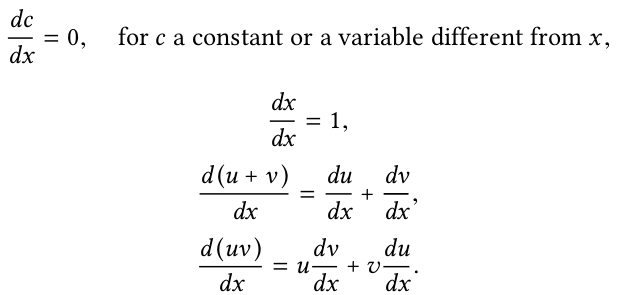
\includegraphics[scale = 0.3]{assets/derivative.png}
\end{center}
Observe that the later two rules are recursive in nature. at is, to obtain the derivative of a sum we first find the derivatives of the terms and add them. Each of the terms may in turn be an expression that needs to be decomposed. Decomposing into smaller and smaller pieces will eventually produce pieces that are either constants or variables, whose derivatives will be either 0 or 1.
\begin{proposition}
    To embody these rules in a procedure we indulge in a little wishful thinking, as we did in designing the rational-number implementation. if we had a means for representing algebraic expressions, we should be able to tell whether an expression is a sum, a product, a constant, or a variable. We should be able to extract the parts of an expression.
\end{proposition}
That is when you write this symbolic differentiation program you should start with writing what you want it to do, WiSHiNG the tools you use already exists:
\begin{lstlisting}
def deriv(exp, var: str):
    if is_constant(exp, var):
        return '0'
    elif is_same_variable(exp, var):
        return '1'
    elif is_sum(exp):
        return make_sum(deriv(a1(exp), var), deriv(a2(exp), var))
    elif is_prod(exp):
        return make_sum(
            make_prod(deriv(a1(exp), var), a2(exp)),
            make_prod(a1(exp), deriv(a2(exp), var)),
        )
\end{lstlisting}
This \texttt{deriv} procedure incorporates the complete differentiation algo rithm. Since it is expressed in terms of abstract data, it will work no matter how we choose to represent algebraic expressions, as long as we design a proper set of selectors and constructors. Then you write your tools:
\begin{lstlisting}
    from string import ascii_letters
    from typing import List
    
    
    def is_equal(exp, var: str) -> bool:
        return exp[0] == var
    
    def is_atom(exp) -> bool:
        return isinstance(exp,str) and (exp in ascii_letters or exp.isnumeric())
    
    def a1(exp):
        return exp[1][0]
    
    def a2(exp):
        return exp[1][1]
    
    def make_sum(a1, a2):
        return '+' + '(' + a1 + ' '+ a2 + ')'
    
    def make_prod(m1, m2):
        return '*' + '(' + m1 +' '+ m2+ ')'
    
    def is_constant(exp, var: str) -> bool:
        return is_atom(exp) and not is_equal(exp, var)
    
    def is_same_variable(exp, var: str) -> bool:
        return is_atom(exp) and is_equal(exp,var)
    
    def is_sum(exp) -> bool:
        return not is_atom(exp) and exp[0] == '+'
    
    def is_prod(exp) -> bool:
        return not is_atom(exp) and exp[0] == '*'
\end{lstlisting}

For example running:
\begin{lstlisting}
deriv(['*',['x', 'x']],'x')
\end{lstlisting}
returns:
\begin{lstlisting}
'+(*(1 x) *(x 1))'
\end{lstlisting}
or running
\begin{lstlisting}
deriv(['*',['x', 'y']],'x')
\end{lstlisting}
returns:
\begin{lstlisting}
deriv(['*',['x', 'y']],'x')
\end{lstlisting}
The program produces answers that are correct; however, they are unsimplified.
Our difficulty is much like the one we encountered with the rational number implementation: we haven't reduced answers to simplest form. To accomplish the rational-number reduction, we needed to change only the constructors and the selectors of the implementation. We can adopt a similar strategy here. We won't change deriv at all. instead, we will change \texttt{make-sum} so that if both summands are numbers, make-sum will add them and return their sum. Also, if one of the summands is 0, then make-sum will return the other summand.
\begin{lstlisting}
def make_sum(a1, a2):
    if a1.isnumeric() and a2.isnumeric():
        return str(int(a1) + int(a2))
    return '+' + '(' + a1 + ' '+ a2 + ')'

def make_prod(m1, m2):
    if m1.isnumeric() and m2.isnumeric():
        return str(int(m1) * int(m2))
    return '*' + '(' + m1 +' '+ m2+ ')'
\end{lstlisting}
Then:
\begin{lstlisting}
deriv(['+',['x', 'x']],'x') returns '2'
\end{lstlisting}
The real story is that we have chosen the expressions in our language which does symbolic calculations to be the same as the representation in the language I am writing the code (Python). By doing so, I have invoked the necessity to have things like \textbf{quotation}. Because of the fact that the outer language is capable of writing expressions that talk about expressions of my language, I need to have something that says, \texttt{"+"} is an expression rather than the operation \texttt{+}. Given that power, if I can manipulate expressions of the language, I can begin to build even more powerful layers upon layers of languages. Because I can write languages that are not only embedded in Lisp/Python, but languages that are completely different, that are \textbf{interpreted} in Lisp/Python. We have hit a line that gives us tremendous power.

\subsection{Example: Representing Sets}
in the previous examples we built representations for two kinds of compound data objects: rational numbers and algebraic expressions. in one of these examples we had the choice of simplifying (reducing) the expressions at either construction time or selection time, but other than that the choice of a representation for these structures in terms of lists was straightforward. When we turn to the representation of sets, the choice of a representation is not so obvious. indeed, there are a number of possible representations, and they differ significantly from one another in several ways.
\begin{definition}
    informally, set is simply a collection of distinct objects. To give a more precise definition we can employ the method of data abstraction. That is, we define "set” by specifying the operations that are to be used on sets. These are union-set , intersection-set , element-of-set? , and adjoin-set .
\end{definition}
From the viewpoint of data abstraction, we are free to design any representation that implements these operations in a way consistent with the interpretations given above.
\subsection{Sets as unordered lists}
One way to represent a set is as a list of its elements in which no element appears more than once.
\begin{lstlisting}
    class Set:
        def __init__(self):
            self.set = []
        def contains(self, x):
            return x in self.set
        def adjoin(self, x):
            if not self.set.contains(x):
                self.set.append(x)
        def intersect(self, other):
            intersection = []
            for e1 in self.set:
                for e2 in other.set:
                    if e1 == e2:
                        intersection.append(e1)
            return intersection
\end{lstlisting}
in designing a representation, one of the issues we should be concerned
with is efficiency.
\texttt{contains} is linear , \texttt{intersect} is quadratic.

\subsection{Sets as ordered lists}
One way to speed up our set operations is to change the representation so that the set elements
are listed in increasing order. To do this, we need some way to compare two objects so that
we can say which is bigger. For example, we could compare symbols lexicographically, or we
could agree on some method for assigning a unique number to an object and then compare the
elements by comparing the corresponding numbers. To keep our discussion simple, we will consider
only the case where the set elements are numbers. improvements include:
\begin{itemize}
    \item binary search for the contains method
    \item using two pointers for intersect will lead to linear time (instead of quadratic)
\end{itemize}

\subsection{Sets as binary search trees}
We can do better than the ordered-list representation by arranging the set elements in the form
of a tree. Each node of the tree holds one element of the set, called the "entry” at that node,
and a link to each of two other (possibly empty) nodes. The "left” link points to elements smaller
than the one at the node, and the "right” link to elements greater than the one at the node.
The advantage of the tree representation is this: Suppose we want to
check whether a number x is contained in a set. We begin by comparing
x with the entry in the top node. if x is less than this, we know that we
need only search the left subtree; if x is greater, we need only search
the right subtree. Now, if the tree is "balanced,” each of these subtrees
will be about half the size of the original. Thus, in one step we have
reduced the problem of searching a tree of size n to searching a tree
of size n/2. Since the size of the tree is halved at each step, we should
expect that the number of steps needed to search a tree of size n grows
as $\Theta(log n)$.
Adjoining an item to a set is implemented similarly and also requires $\Theta(log n)$ steps.
To adjoin an item x , we compare x with the node entry to determine whether x should be added to
the right or to the left branch, and having adjoined x to the appropriate branch we piece this
newly constructed branch together with the original entry and the other branch.

\section{Lecture 4A: Pattern Matching and Rule-based Substitution}
This is covered only in video not in book.
Questioning why we would translate the calculus rules into the language of the computer.
Is there a way to write the DERIV program that is more clear? Before we had to do dispatching on type
If we compute a derivative on a constant do this, else do that, etc. This lecture  it introduces
ideas around creating a language for dealing with \href{https://en.wikipedia.org/wiki/Eval}{eval}
rules and then using eval as a way to simplify rules.
All the calculus rules have a left hand and right hand side.
Given a Pattern, we use a rule to produce a skeleton.
Pattern is matched against an expression, application of rule produces a new expression that is an
instantiation of a skeleton.
Goal: Build a language that will allow the computer to understand these rules.


\section{Lecture 4B: Generic Operators}
So far we have been talking a lot about data abstractions. We build systems which have horizontal
barriers which separate use and representation of data objects. This give you the chance to think
about the separately. For example Boss uses data structures, George builds the representations.
This is powerful but not enough. We might have many Georges, or in particular we might have a
company is formed by merging different companies with different databases and systems. Each
division would have different way of their databases, they have different representation of their
data! We want to have a unified way of using data with different representations.
\subsection{Multiple Representations for Abstract Data}
We have introduced data abstraction, a methodology for structuring
systems in such a way that much of a program can be specified independent of the choices involved
in implementing the data objects that the program manipulates.
The key idea was to erect an abstraction barrier—in this case, the selectors and constructors for
rational numbers \texttt{(make-rat, numer, denom)} —
that isolates the way rational numbers are used from their underlying
representation in terms of list structure. A similar abstraction barrier
isolates the details of the procedures that perform rational arithmetic
\texttt{(add-rat, sub-rat, mul-rat, and div-rat)} from the "higher-level” procedures that use
rational numbers. These data-abstraction barriers are powerful tools for controlling complexity.
But this kind of data abstraction is not yet powerful enough. We might want to have multiple
representations of the same data object. To take a simple example, complex numbers may be
represented in two almost equivalent ways: in rectangular form (real and imaginary parts) and in
polar form (magnitude and angle).
\begin{proposition}
    So in addition to the data-abstraction barriers that isolate representation from use, we need
    abstraction barriers that isolate different design choices from each other and permit different
    choices to coexist in
    a single program.
\end{proposition}
Furthermore, since large programs are often created by combining pre-existing modules that were
designed in isolation, we need conventions that permit programmers to incorporate modules into larger
systems additively, that is, without having to redesign or reimplement these modules. \newline
in this section, we will learn how to cope with data that may be
represented in different ways by different parts of a program. This requires constructing
\textbf{generic procedures} —procedures that can operate on data that may be represented in
more than one way. Our main technique for building generic procedures will be to work in terms
of data objects that have type \textbf{tags} (framework by Toshko), that is, data objects that
include explicit information about how they are to be processed. We will also discuss
\textbf{data-directed} programming, a powerful and convenient implementation strategy for
additively assembling systems with generic operations.

\subsection{Representation for Complex Numbers}
We begin with the simple complex-number example. We will see how \\ \textbf{type tags}
and \textbf{data-directed style} enable us to design separate rectangular and polar
representations for complex numbers while maintaining
the notion of an abstract "complex-number” data object. We will accomplish this by defining
arithmetic procedures for complex numbers \texttt{(add-complex, sub-complex, mul-complex, and div-complex)}
in terms of generic selectors that access parts of a complex number independent of how the number
is represented.
The resulting complex-number system, as shown in Figure 2.19, contains two different kinds of
abstraction barriers.
The "horizontal" abstraction barriers play the same role as the ones in Figure 2.1.
They isolate "higher-level" operations from "lower-level" representations.
in addition, there is a "vertical” barrier that gives us the ability to separately
design and install alternative representations.

\begin{center}
    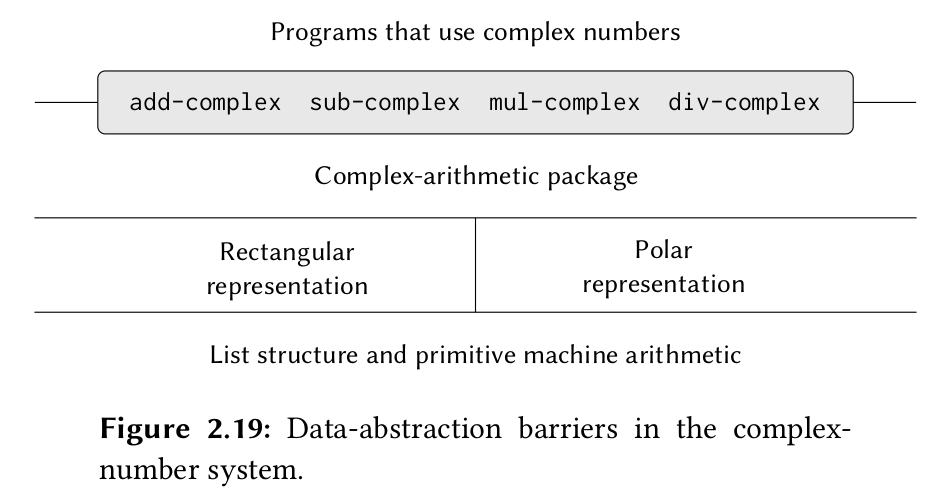
\includegraphics[scale=0.5]{assets/complex_numbers_abs.png}
\end{center}

Like rational numbers, complex numbers are naturally represented as ordered pairs. Addition of complex
numbers reduces in this representation to addition
of coordinates:
\begin{center}
    Real-part($z_1 + z_2$) = Real-part($z_1$) + Real-part($z_2$),
    imaginary-part($z_1$ + $z_2$) = imaginary-part($z_1$) + imaginary-part($z_2$)
\end{center}
When multiplying complex numbers, it is more natural to think in
terms of representing a complex number in polar form, as a magnitude
and an angle
\begin{center}
    Magnitude($z_1$ · $z_2$) = Magnitude($z_1$) · Magnitude($z_2$),
    Angle($z_1$ · $z_2$) = Angle($z_1$) + Angle($z_2$)
\end{center}
Thus, there are two different representations for complex numbers, which are appropriate for different
operations. Yet, from the viewpoint of someone writing a program that uses complex numbers, the principle
of data abstraction suggests that all the operations for manipulating complex numbers should be available
regardless of which representation is used by the computer. Our goal is albeit the different
representation of complex numbers to be able to do arithmetic operations on the:
\begin{center}
    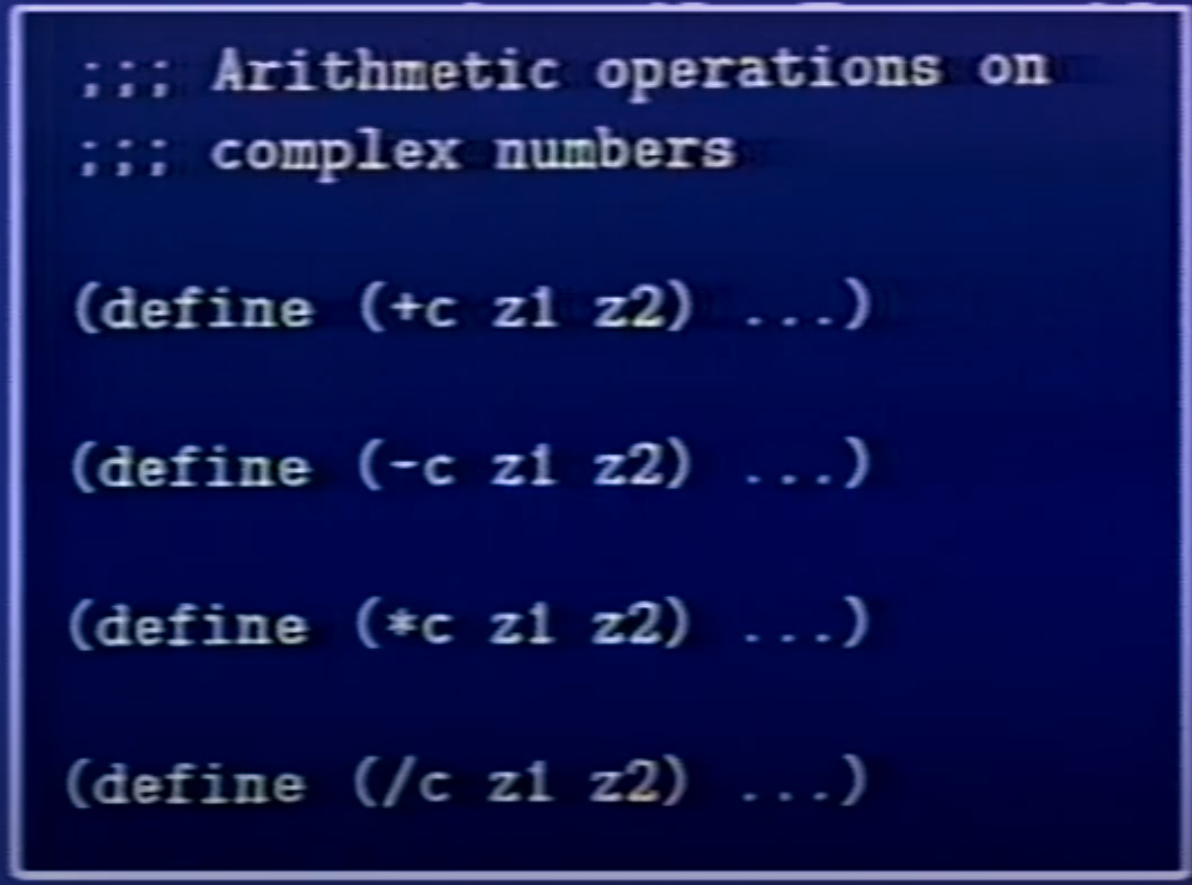
\includegraphics[scale=0.12]{assets/arithmetic_ops.png}
\end{center}
in order to make the different choices concrete, imagine that there are two programmers, Ben Bitdiddle
and Alyssa P. Hacker, who are independently designing representations for the complex-number system.
Ben chooses to represent complex numbers in rectangular form whereas Alyssa chooses to represent
complex numbers in polar form. Below is an implementation in Python which encapsulates both representations
in one and Alyse and Ben can use all methods regardless of their choice of complex number representation:
\begin{lstlisting}[language=Python]
import math

class ComplexNumber:
    def __init__(self, val1, val2, representation='rect'):
        if representation == "rect":
            self.real = val1
            self.imaginary = val2
            self.mag = math.sqrt(val1**2+val2**2)
            self.angle = math.atan(val2/val1)
        elif representation == 'polar':
            self.mag = val1
            self.angle = val2
            self.real = val1*math.cos(val2)
            self.imaginary = val1*math.sin(val2)
        else:
            raise ValueError("invalid representation")

    def __str__(self):
        if self.imaginary == 0:
            return str(self.real)
        elif self.real == 0:
            return str(self.imaginary)+"i"
        elif self.imaginary > 0:
            return str(self.real)+"+"+str(self.imaginary)+"i"
        else:
            return str(self.real)+str(self.imaginary)+"i"

    def __repr__(self) -> str:
        return str(self)

    def __add__(self,other):
        return ComplexNumber(self.real+other.real,self.imaginary+other.imaginary)

    def __sub__(self,other):
        return ComplexNumber(self.real-other.real,self.imaginary-other.imaginary)

    def __mul__(self,other):
        return ComplexNumber(self.mag*other.mag,self.angle+other.angle,representation='polar')

    def __divide__(self,other):
        return ComplexNumber(self.mag/other.mag,self.angle-other.angle,representation='polar')

    def __abs__(self):
        return self.mag

    def __eq__(self,other):
        return self.real == other.real and self.imaginary == other.imaginary

    def __ne__(self,other):
        return self.real != other.real or self.imaginary != other.imaginary

    def __gt__(self,other):
        return self.mag > other.mag

    def __ge__(self,other):
        return self.mag >= other.mag

    def __lt__(self,other):
        return self.mag < other.mag

    def __le__(self,other):
        return self.mag <= other.mag

    def __neg__(self):
        return ComplexNumber(self.real,self.imaginary*-1)

    def __pos__(self):
        return ComplexNumber(self.real,self.imaginary)

    def __invert__(self):
        return ComplexNumber(self.mag,self.angle+math.pi,representation='polar')

\end{lstlisting}

\subsection{Tagged data}
When having two representations in one system we need to distinguish between them. Our above solution
is straightforward way to accomplish this distinction by a \textbf{type tag} (we call
\texttt{representation}) — the symbol \texttt{rectangular} or \texttt{polar} — as part of
each complex number. Then when we need to manipulate a complex number we can use the tag to decide
which selector to apply. Note that having the two representations
is beneficial for us as some methods like addition are better computed using rectangular form
and other like multiplication, greater, smaller are better computed using polar form.
One way to view data abstraction is as an application of the "principle of least commitment.”
in implementing the complex-number system in Section 2.4.1, we can use either Ben's rectangular
representation or Alyssa's polar representation. The abstraction barrier formed by the selectors
and constructors permits us to defer to the last possible moment the choice of a concrete
representation for our data objects and thus retain maximum flexibility in our system design.
The principle of least commitment can be carried to even further extremes. if we desire,
we can maintain the ambiguity of representation even after we have designed the selectors and
constructors, and elect to use both Ben's representation and Alyssa's representation.
Whenever Ben constructs a complex number, he tags it as rectangular. Whenever
Alyssa constructs a complex number, she tags it as polar.
\begin{center}
    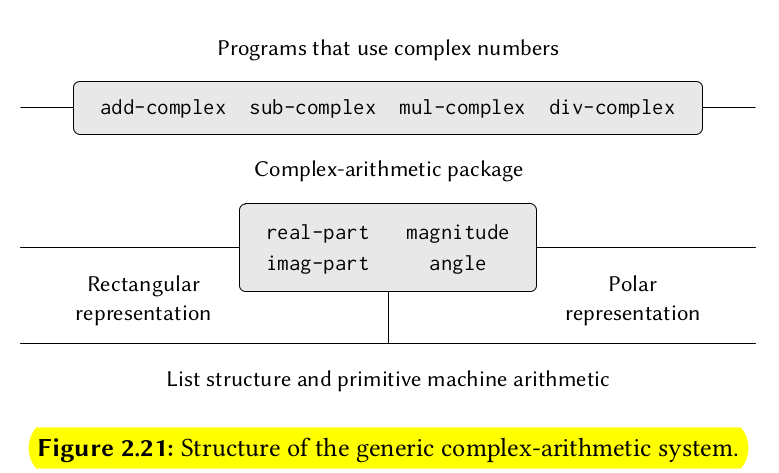
\includegraphics[scale=0.12]{assets/complex_number_structure.png}
\end{center}
The resulting complex-number system has the structure shown in Figure 2.21. e system has been
decomposed into three relatively independent parts: the complex-number-arithmetic operations,
Alyssa's polar implementation, and Ben's rectangular implementation. The polar and rectangular
implementations could have been written by Ben and Alyssa working separately, and both of these
can be used as underlying representations by a third programmer implementing the complex-arithmetic
procedures in terms of the abstract constructor/selector interface. Since each data object is tagged
with its type, the selectors (getters) and the arithmetic methods operate on the data in a generic
manner. That is, each selector is defined to have a behavior that depends upon the particular
type of data it is applied to.
\subsection{Data-Directed Programming and Additivity}
The general strategy of checking the type of a datum and calling an
appropriate procedure is called \texttt{dispatching on type}. This is a powerful strategy for
obtaining modularity in system design.
\begin{definition}
    Dynamic dispatch is the process of selecting which implementation of a polymorphic operation
    (method or function) to call at run time. it is commonly employed in, and considered a prime
    characteristic of, object-oriented programming (OOP) languages and systems.
\end{definition}
Object-oriented systems model a problem as a set of interacting objects that enact operations
referred to by name. \textbf{Polymorphism} is the phenomenon wherein somewhat interchangeable objects
each expose an operation of the same name but possibly differing in behavior.
\begin{proposition}
    Dynamic dispatch contrasts with static dispatch, in which the implementation of a polymorphic
    operation is selected at compile time. The purpose of dynamic dispatch is to defer
    the selection of an appropriate implementation until the run time type of a parameter
    (or multiple parameters) is known.
\end{proposition}
\begin{definition}
    Static dispatch is a form of polymorphism fully resolved during compile time. it is a form of
    method dispatch, which describes how a language or environment will select which implementation
    of a method or function to use.
\end{definition}
Dynamic dispatch will always incur an overhead so some languages offer static dispatch for particular
methods. A language may be implemented with different dynamic dispatch mechanisms.
The choices of the dynamic dispatch mechanism offered by a language to a large extent
alter the programming paradigms that are available or are most natural to use within a given language.
Normally, in a typed language, the dispatch mechanism will be performed based on the type of the
arguments (most commonly based on the type of the receiver of a message). Languages with weak or no
typing systems often carry a dispatch table as part of the object data for each object.
This allows instance behaviour as each instance may map a given message to a separate method.
Example in python of dynamic dispatching:
\begin{lstlisting}[language=Python]
class Cat:
    def speak(self):
        print("Meow")

class Dog:
    def speak(self):
        print("Woof")


def speak(pet):
    # Dynamically dispatches the speak method
    # pet can either be an instance of Cat or Dog
    pet.speak()

cat = Cat()
speak(cat)
dog = Dog()
speak(dog)
\end{lstlisting}
\subsection{Systems with Generic Operations}
Now we will see how to use this same idea not only to define operations that are generic over
different representations but also to define operations that are generic
over different kinds of arguments. That is we would define \texttt{operate(argument1, argument2)}
We are adding abstraction layer over operations, no just data type!
Now we will see how to use this same idea not only to define operations that are generic over
different representations but also to define operations that are generic
over different kinds of arguments.
\begin{center}
    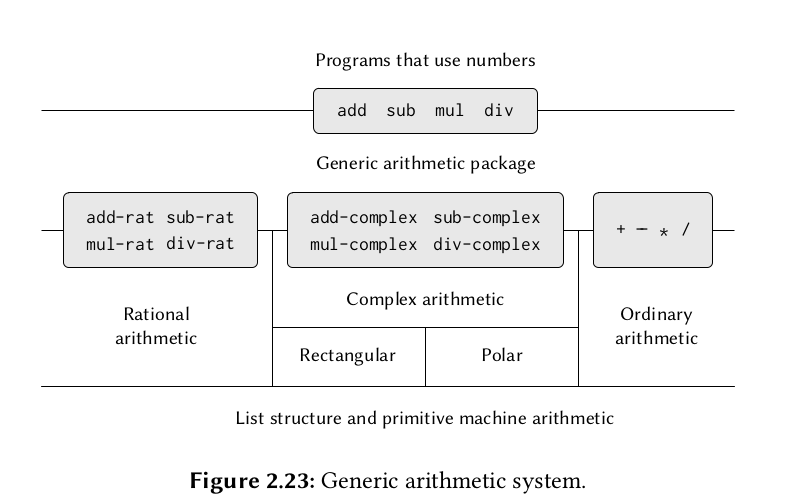
\includegraphics[scale = 0.3]{assets/arithmetic_package_system.png}
\end{center}
We go from top to bottom. For example computing $(3 + 4i)*(1 + 2*i)$ our path in the system would be:
\begin{enumerate}
    \item I have numbers $3 + 4i$, $1 + 2i$
    \item I need to use generic arithmetic multiply complex
    \item Are these complex numbers Rectangular or Polar?
\end{enumerate}
Each time we go to a level we use the type of our object, and send it through the different levels
using dispatching and message passing.
\begin{center}
    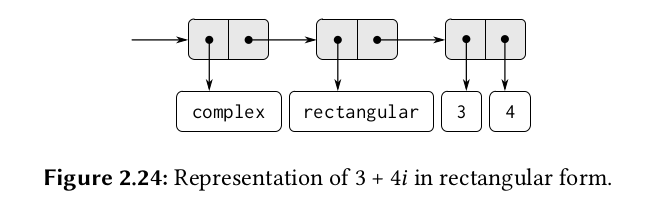
\includegraphics[scale = 0.3]{assets/repre_complex.png}
\end{center}
As a data objectis passed "downward", the outer tag that is used to direct it to the ap
propriate package is stripped off (by applying contents ) and the next
level of tag (if any) becomes visible to be used for further dispatching.

\subsection{Big Summary}
The two fundamental elements of programming: functions and data are the SAME THiNG.
Functions can be manimulated as data using higher-order procedures (functions which return other
functions). Data can possess the power of doing things and bahaving using message passing and
object system. Current tools for organizing large programs:
\begin{itemize}
    \item functional abstraction
    \item data abstraction
    \item class inheritance
    \item generic functions
\end{itemize}
Effective program synthesis also requires organizational principles that
can guide us in formulating the overall design of a program. in partic-
ular, we need strategies to help us structure large systems so that they
will be \textbf{modular} , that is, so that they can be divided “naturally” into co-
herent parts that can be separately developed and maintained.

\section{Lecture 5A: Assignment, State, and Environmental model.}
In next 3 lectures we will investigate two prominent organizational strategies arising from
two rather different “world views” of the structure of systems.
The first organizational strategy concentrates on objects , viewing a large system
as a collection of distinct objects whose behaviors may change over
time. An alternative organizational strategy concentrates on the streams
of information that flow in the system, much as an electrical engineer
views a signal-processing system. So far we haven't used any assignment
statement, we have written \textbf{functional programs} which are \textbf{encoded mathematical truths}.
Processes evolved by such programs can be understood by substitution:

\begin{lstlisting}[language=Python]
    (fact 3)
    (* 3 (fact 2))
    (* 3 (* 2 (fact 1)))
    (* 3 (* 2 1))
    (* 3 2)
    6
\end{lstlisting}

\subsection{Assignment kills the substitution model}
An \textit{assignment} creates a moment in time. Introducing it to our language totally kills the substitution model. We can no longer just substitute values into
the expression we want to evaluate.
\begin{lstlisting}[language=Python]
    count = 1
    def demo(x):
        count = count + 1
        return x + count
    print(demo(3)) # prints 5
    print(demo(3)) $ prints 6
\end{lstlisting}
The substitution model is dead, we cannot substitue for count as it changes. The substituteion model accounts
for static states. We have lost our model of computation\dots
\begin{proposition}
    Thus, when we have something like assignment. The model we need a model which would refer to the
    symbols \texttt{x} and \texttt{count} would no longer refer to the values, but rather to some
    adresses where the value is stored.
\end{proposition}
This addressing is a pain in the ass, really bad thing. Apart from losing our simple model of computation
we also loose the notion of samenes and equal. Thus Python have different meaning when checking $==$
and object1 $ is$ object2. A language that supports the concept that “equals can be substituted for
equals” in an expression without changing the value of the expression is said to be referentially
transparent. Referential transparency is violated when we include set! in our computer language.
This makes it tricky to determine when we can simplify expressions by substituting equivalent
expressions. Consequently, reasoning about programs that use assignment becomes drastically
more difficult. We need a really good reason to introduce assignment.
\begin{lstlisting}[language=Python]
    def fact(n):
    """Functional program"""
        def iter(m, i):
            if I > n: return m
            else: iter(i*m,i+1)
        return iter(1,1)
    def fact(n):
    """imperative program"""
        res = 1
        for I in range(1,n+1):
            res *= i
        return res
\end{lstlisting}
Programming without any use of assignments, as we did throughout
the first two chapters of this book, is accordingly known as \textit{functional programming}.
So we do not actually need to have assignment to write large programs.
\begin{definition}
    Assignment destroys all our mathematical properties of our programs
\end{definition}

\subsection{The Environment Model of Evaluation}
Viewing systems as collections of objects with local state is a powerful technique for maintaining
a modular design. This is a new model for understanding the execution of programs.
We need a new model of computation called \textbf{environment model} where assignment would work.
The presence of assignment, a variable can no longer be considered to be
merely a name for a value. Rather, a variable must somehow designate
a “place” in which values can be stored. in our new model of evaluation,
these places will be maintained in structures called \textit{environments}.
\begin{definition}
    An environment is a sequence of frames . Each frame is a table (possibly empty) of bindings,
    which associate variable names with their corresponding values.
\end{definition}
Each frame also has a pointer to its enclosing environment, unless,
for the purposes of discussion, the frame is considered to
be global. The value of a variable with respect to an environment is the
value given by the binding of the variable in the first frame in
the environment that contains a binding for that variable
\begin{center}
    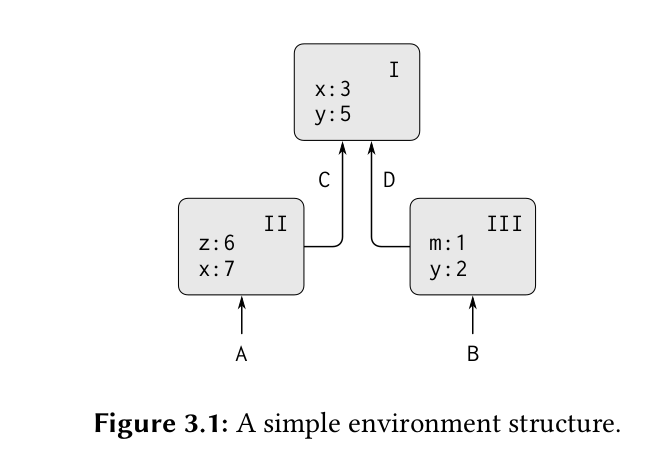
\includegraphics[scale = 0.4]{assets/environment_structure.png}
\end{center}
Figure 3.1 shows a simple environment structure consisting of three
frames, labeled i, ii, and iii. in the diagram, A, B, C, and D are pointers to
environments. C and D point to the same environment. Thee variables z
and x are bound in frame ii, while y and x are bound in frame i. The value
of x in environment D is 3. The value of x with respect to environment
B is also 3. This is determined as follows: We examine the first frame in
the sequence (frame iii) and do not find a binding for x , so we proceed
to the enclosing environment D and find the binding in frame i. On the
other hand, the value of x in environment A is 7, because the first frame
in the sequence (frame ii) contains a binding of x to 7. With respect to
environment A, the binding of x to 7 in frame ii is said to shadow the
binding of x to 3 in frame i.
\begin{definition}
    The environment is the linked chains of frames.
\end{definition}
\subsection{The benefits and disadvantages of Assignment}
\begin{proposition}
    Assignment serves the purpose to \textbf{bind} name to a value. Gives you another way
    to name your spells and invoke them.
\end{proposition}


Assignment allows us to have different computational objects which have similar
attributes but the state of these attributes may differ. We like to think absolute
objects because it is economical. You are object, I am object. We both have similar state variables
such as blood pressure, temperature. We as objects can interact with each other affecting each others
states. Most of the things around us are objects, it is the way we think about the world around us.
However it may not be always appropriate to think about the world as independent states and
independent particles.When I have assignments I can change state of variables. When I do not have
assignment and everything is a function they cannot change their local states.
By introducing assignment and objects we have opened ourselves up to all horrible
questions of philosophy such as what is identity of an object. When two objects are the same?
if an object change is it the same or is it different? If I break my nail am I the same one? I am me
but I am slightly different. Mathematics is much cleaner and we have destroyed it with assignments.
\newline
\begin{itemize}
    \item Assignment gives you the power to make independent local state and to model objects
    \item Assignment is a simple means of abstraction, for it allows us to use simple names to
          refer to the results of compound operations, such as the area computed above.
    \item Assignment destroys the substitution model which has solid mathematical foundations.
          The equal sign is does not mean equal anymore.
    \item Assignment introduces the notion of \textbf{time and identity} of objects which is main source of bugs.
\end{itemize}
Having objects with variable states can be beneficial if you want objects to change their state.
However, there are cases when you want to have fixed things.
\begin{lstlisting}[language=Python]
    a = [1,2,3]
    obj = [a,a]
    a[0] += 1
\end{lstlisting}
Then object \texttt{obj} has changed his values when we changed the list \texttt{a}!
Assignment introduces interactions between objects. This is the source of most bugs in a large
computer program. By introducing the ability things can have identity sharing states
and having the same names but refer to different objects, we get a lot of power but pay with complexity
and bugs.

\subsection{Summary}
The consequences of introducing assignment is that we have to worry about:
\begin{itemize}
    \item state of the objects
    \item change in the objects
    \item time of change
    \item identity
    \item sharing
\end{itemize}
A variable is not something that stands for a value, it stands for a place holding a value which can change.
Suddenly we have to think not only about values but \textbf{about time}.
We ended up with this mess because we were trying to build a \textbf{modular system}, decomposed into \textbf{natural
    pieces} (cfr digital circuit).

\section{Lecture 5B: Computational Objects. OOP vs Functional}
OOP gives you relationship between the object in the worlds and the object models in the computer.
This buys us modularity. We want our computational world to have objects with independent local states
and relations between each other which resemble the actual world.
OOP allows you to make complex event-driven simulation where the objects in the world are
the objects in the computer. The changes of state that are happening in the world in \textbf{time} are
organized to be time in the computer, so that if something happens after something else in the world,
then we have it happen after the corresponding events in the computer. That's why we have
\textit{assignments}.
\subsection{OOP vs Functional}
Functional programming does follow the declarative programming model. OOP does follow the imperative
programming model. Example of declarative programming model is when you created a language for
computing symbolic derivative calculation.
Two questions are important when comparing these two different paradigms.
\begin{itemize}
    \item When do you choose functional programming over object-oriented?
    \item What are the typical problem definitions where functional programming is a better choice?
\end{itemize}
When you anticipate a different kind of software evolution:
\begin{itemize}
    \item Object-oriented languages are good when you have a fixed set of operations on things,
          and as your code evolves, you primarily add new things. This can be accomplished by
          adding new
          classes which implement existing methods, and the existing classes are left alone.
    \item Functional languages are good when you have a fixed set of things, and as your
          code evolves, you primarily add new operations on existing things. This can be accomplished by
          adding new functions which compute with existing data types, and the existing functions are left
          alone.
\end{itemize}

When evolution goes the wrong way, you have problems:
\begin{itemize}
    \item Adding a new operation to an object-oriented program may require editing many class
          definitions to add a new method.
    \item Adding a new kind of thing to a functional program may require editing many function
          definitions to add a new case.
\end{itemize}
Functional languages excel at manipulating symbolic data in tree form. A favorite example is compilers,
where source and intermediate languages change seldom (mostly the same things), but compiler writers
are always adding new translations and code improvements or optimizations (new operations on things).
Compilation and translation more generally are "killer apps" for functional languages.
Functional programming is the form of programming that attempts to avoid changing state and mutable
data. In a functional program, the output of a function should always be the same, given the same exact
inputs to the function. This is because the outputs of a function in functional programming purely
relies on arguments of the function, and there is no magic that is happening behind the scenes.
This is called eliminating \textbf{side effects} in your code at the cost of giving up assignment and
time. Both Functional programming and object-oriented
programming uses a different method for storing and manipulating the data.
In functional programming, data cannot be stored in objects and it can only be transformed by
creating functions. In object-oriented programming, data is stored in objects.
Unit testing in OOP is harder. Objects may maintain internal state, which is not easily accessible by the tests.\\
Purely Functional Programming $=>$ no-side effects (constant states), no synchronization problems
at the price of giving up assignment

\section{Lecture 6A: Streams, Part 1}
Here we discuss developing new tools to process sequential data.
Streams offer another way to represent sequential data implicitly. A stream is a lazily computed linked list.
\textbf{Stream processing} is another way of building modular system. We want our programs to worry
less about \textbf{time}. Consider the two problems:
\begin{itemize}
    \item Given a tree return the sum of squares of all leaves with odd values.
    \item Given the first n Fibonacci numbers return the sum of the odd ones.
\end{itemize}

\begin{lstlisting}
| enumerate leaves |-->| filter odd? |-->| map square |-->| accumulate + init 0 |
\end{lstlisting}

\begin{lstlisting}
| enum interval |-->| map fib |-->| filter odd? |-->| accumulate + init [] |
\end{lstlisting}
\begin{lstlisting}[language=Python]
    # Problem 1
    # Input data needs to be enumerated as a a stream!
    class TreeNode:
        def __init__(self, val = None, left = None, right = None):
            self.val = val
            self.left = left
            self.right = right

    # Tree iterator would be more efficient in memory (leetcode problem)
    def enum(root):
        if root:
            if root.left is None and root.right is None:
                yield root.val
            for leaf in  enum(root.left):
                yield leaf
            for leaf in  enum(root.right):
                yield leaf

    def isodd(n):
        return n % 2 == 1

    def square(n):
        return n*n

    def enum(root):
        if root.left is None and root.right is None:
            return [root.val]
        l = enum(root.left)
        r = enum(root.right)
        print(l,r)
        return l+r
    n = 5
    root = create_tree(n)
    sum(map(square,filter(isodd,enum(root))))

    # Problem 2
    from functools import lru_cache
    @lru_cache
    def fib(n):
        if n <= 1: return n
        return fib(n-1)+fib(n-2)

    def enum(n):
        return range(n+1)

    def isodd(num):
        return num % 2 ==1


    n = 15
    # Input data needs to be enumerated as a a stream!
    input_stream = enum(n)
    tuple(filter(isodd,map(fib,input_stream)))
\end{lstlisting}

Why is this simpler? With streams we threw away the idea that the above two processes happen in time
with changing state (summation and appending). We said it is a whole collection of stuff. Wwe have
changed our view of how we model the world - instead of having state and time, we try to model globally.

\subsection{Efficient Stream Programs}
Problem: find the second prime between 10,000 and 1,000,000:
\begin{lstlisting}[language=Lisp]
(head
  (tail
    (filter
        prime?
        (enum-interval 10000 1000000))))
\end{lstlisting}
The power of the ugly non-stream programming style is its weakness: we are mixing up the enumerating,
the testing and the accumulating - where we do not need to consider the whole stream. To optimize note:
\textbf{Streams Are Not Lists}
\begin{proposition}
    We want streams to be a data structure which computes itself incrementally, an on-demand data structure.
\end{proposition}
Streams are data structures are in fact sort of like procedures. another proof there is no clear dividing
line between data and procedures.

\begin{proposition}
    Any amount of side-effect will mess up everything unless you are very careful.
\end{proposition}


\subsection{N Queens problem}
Instead of doing backtracking we can filter out the non-violating conditions permutations of the board:

\begin{lstlisting}[language=Python]
from itertools import permutations

class Solution(object):
    def goodPerm(self, p):
        n = len(p)
        for i in range(n-1):
            for j in range(i+1, n):
                if abs(p[i] - p[j]) == j - i:
                    return False
        return True
    
    def totalNQueens(self, n):
        good = list(filter(self.goodPerm, permutations(range(n))))
        return len(good)
\end{lstlisting}
Of course this is slower than backtracking, but much cleaner. That's because we don't have the notion
of time here.

\subsection{Lecture 6B: Streams, Part 2}
The key idea behind streams is to offer a mean of decoupling the apparent
order of events in our program to the actual order of events in the computer.
We can deal with very long streams and generate elements on demand.

\begin{lstlisting}[language=Python]
class Stream:
    """A lazily computed linked list."""
    class empty:
        def __repr__(self):
            return 'Stream.empty'

    def _compute_rest1():
        empty = Stream.empty()
        return empty

    def __init__(self,first, compute_rest = _compute_rest1):
        assert callable(compute_rest)
        self.first = first
        self._compute_rest = compute_rest

    @property
    def rest(self):
        """Return the rest of the stream, computing it if necessary."""
        if self._compute_rest is not None:
            self._rest = self._compute_rest()
            self._compute_rest = None
        return self._rest

    def __repr__(self):
        return f'Stream({repr(self.first)}, <...>)'
\end{lstlisting}


\subsection{Infinite Streams}
The essential properties of a \texttt{compute\_rest} function are that it takes no arguments, and
it returns a Stream or Stream.empty.
Lazy evaluation gives us the ability to represent infinite sequential datasets using streams. For example, we can represent increasing integers, starting at any first value.

\begin{lstlisting}[language=Python]
def integer_stream(first):
    def compute_rest():
        return integer_stream(first+1)
    return Stream(first, compute_rest)
\end{lstlisting}
We can \texttt{map} and \texttt{filter} streams as we did with other representations of sequences.
We need to do that lazily.

\begin{lstlisting}[language=Python]
def map_stream(fn, s):
    if s is Stream.empty:
        return s
    def compute_rest():
        return map_stream(fn, s.rest)
    return Stream(fn(s.first), compute_rest)

def filter_stream(fn, s):
    if s is Stream.empty:
        return s
    def compute_rest():
        return filter_stream(fn, s.rest)
    if fn(s.first):
        return Stream(s.first, compute_rest)
    else:
        return compute_rest()

squares = map_stream(lambda x: x**2, s)
print(squares.rest.rest)

\end{lstlisting}
Creating a generator for primes in the stream programming style
\begin{lstlisting}[language=Python]
def primes(pos_stream):
    def not_divisible(x):
        return x % pos_stream.first != 0
    def compute_rest():
        return primes(filter_stream(not_divisible, pos_stream.rest))
    return Stream(pos_stream.first, compute_rest)

prime_numbers = primes(integer_stream(2))
first_k_as_list(prime_numbers, 10)
\end{lstlisting}


\subsection{Normal order evaluation bs applicative order of evaluation}

We introduce some basic definitions from lambda calculus:
\begin{definition}
A \textbf{redex} is a reducible function expression, e.g. $f(x)$ \newline
A lambda expression has \textbf{normal form} if that contains no redexes.
\end{definition}
Given a lambda expression, there are two primary strategies for reducing it to normal form:
\textbf{normal-order evaluation}, or \textbf{applicative-order evaluation}.

Applicative-order evaluation means that a function's arguments are evaluated before the function is
applied. Python uses this way of evaluating expressions, this creates a recursive tree expression.
The most noticeable effect of applicative-order evaluation is that recursive functions may not terminate.\\

Normal-order evaluation of a lambda expression is the repeated application of the leftmost
reducible function application. The most noticeable effect of using normal-order evaluation is that,
since we evaluate the leftmost function first, arguments to that function are not evaluated (\textbf{lazy evaluation}).\\
Consider this example of computing the average of the doubles of two numbers.
\begin{lstlisting}[language=Python]
    def double(x):
         return x+x
    def average(x,y):
        return (x+y)/2
\end{lstlisting}
Applicative order would evaluate in this way (INSIDE-OUT):
\begin{lstlisting}[language=Lisp]
    double (average 2 4) =>
    double (divide (plus 2 4) 2) =>
    double (divide 6 2) =>
    double 3 =>
    plus 3 3 =>
    6
\end{lstlisting}
Normal order would evaluate in this way (OUTSIDE-IN):
\begin{lstlisting}[language=Lisp]
    (double (average 2 4)) =>
    (plus (average 2 4) (average 2 4)) =>
    (plus (divide (plus 2 4) 2) (average 2 4)) =>
    (plus (divide 6 2) (average 2 4)) =>
    (plus 3 (average 2 4)) =>
    (plus 3 (divide (plus 2 4) 2)) =>
    (plus 3 (divide 6 2)) =>
    (plus 3 3) =>
    6
\end{lstlisting}

\section{Lecture 7A: Metacircular Evaluator}
In this lecture we build an interpreter of Lisp in Lisp!

Programs (your code) is a character string description = spell recipe.
It could look graphical as a wiring diagram:
\begin{center}
    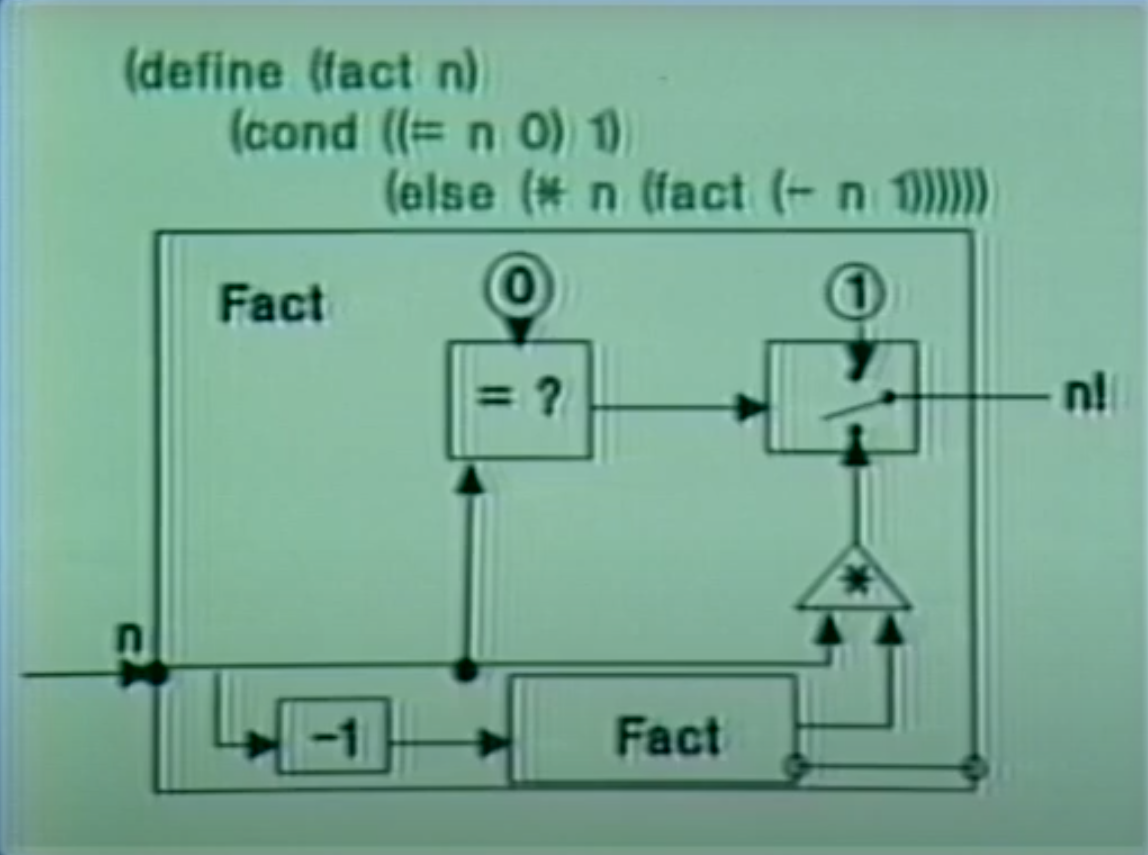
\includegraphics[scale=0.3]{assets/program_diagram.png}
\end{center}

Our computation world has a \textbf{universal machine} called \textbf{eval}.
It takes as input another machine (the wiring diagram).
\begin{center}
    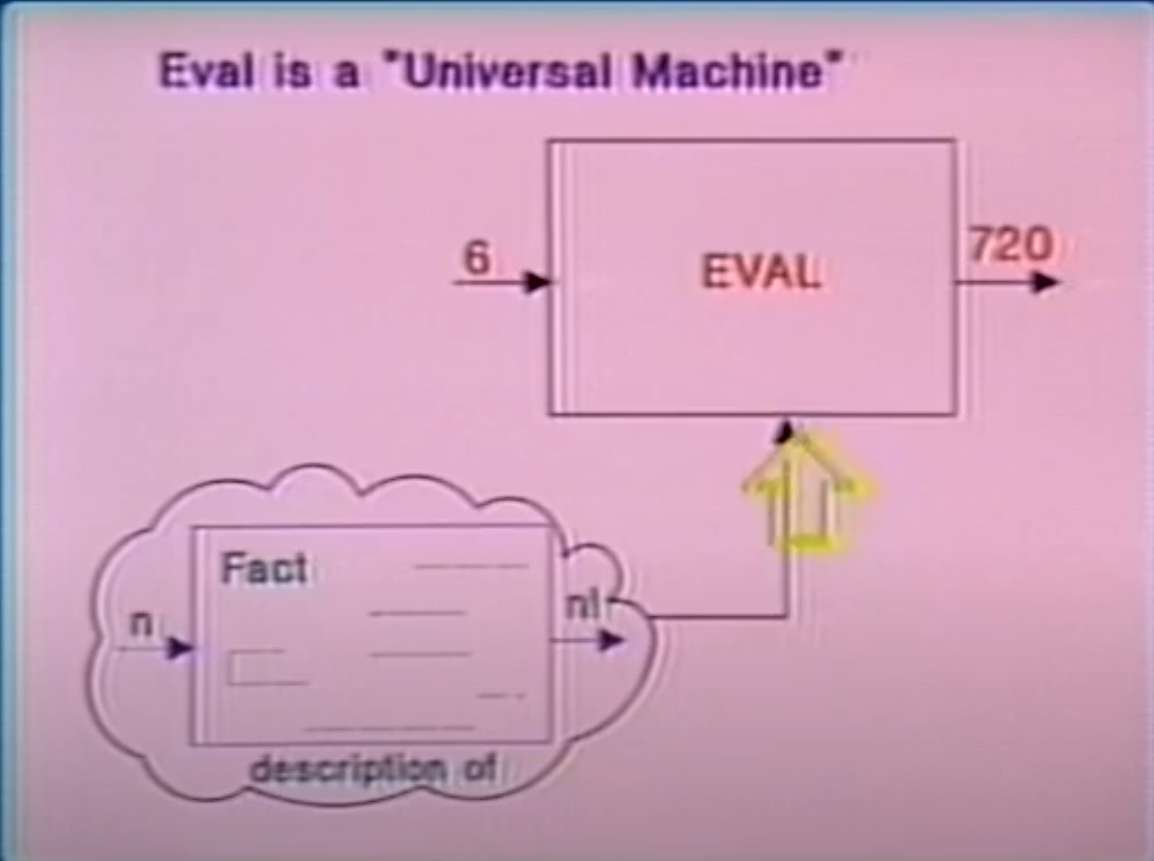
\includegraphics[scale=0.3]{assets/universal machine.png}
\end{center}

Build your own machine:
\begin{lstlisting}[language=Python]
def make_eval():
    def dispatch(expression, env):
        if isnumber(expression):
            return expression # number value expressions should give themselves 3 -> 3
        elif issymbol(expression):
            return look_up_val(expression, env) # if x = 3 and we evaluate expression x -> 3
        elif isstring(expression):
            return expression
        elif islambda(expression):
            '''lambda expressions have: bound variables(arguments), (body), and environment
                (which frame they live)
                Assume they are represented as the class:
                Closure(lambda_argument, lambda_body, env)
            '''
            return [expression.lambda_argument, expression.lambda_body, expression.env]
        elif isconditional(expression):
            return eval_cond(expression.clauses,env)
        else:
            ''' special case such as x + 3'''
            return apply(eval(expression.operand),eval(expression.operators))
    return dispatch
\end{lstlisting}
The eval machine is a case dispatch on the type on the expression, with the default being general
combination (captures cases like x + 3).
\begin{lstlisting}[language=Python]
    def apply(procedure,arguments):
        if isprimitive(procedure):
            return apply_prim_op(procedure, arguments)
        elif iscompound(procedure):
            procedure = transform_to_lambda(procedure,arguments)
            return eval(procedure)
        else:
            raise 'Non existent procedure'

    def eval_cond(clauses,env):
        if isempty(clauses):
            return []
        elif clauses.predicate == True:
            return eval(clauses.first_clause)
        elif clauses.predicate == False:
            return eval_cond(clauses[1:],eval) # recursion

    def look_up(symbol,env):
            if env is empty: return error Unbound variable
            else:
                for frame in env.frames:
                    if find_dfs(symbol, env.frame):
                        # frames have tree structure.
                        return symbol.value
\end{lstlisting}

Methods we need to control/work around the environment model of computation are:
\begin{itemize}
    \item \texttt{bind(var\_name,value)} - it is for making more table/ making a new frame in the environment, where
    the new frame will pair a variable name with  a value
    \item \texttt{pair\_up(var\_name,value,frame)} - add a new pair variablename: value in a given frame.
\end{itemize}

When we evaluate compound expressions we will enter eval ---> apply ---> eval ---> apply loop.

eval takes as input: expression and environment -> produces procedure and arguments for apply
(can do some stuff on its own too in the rest if else statement).

apply takes as input: procedure and arguments -> produces expression and environment.
Do this until we reach primitive expression.

\section{Lecture 7B: Metacircular Evaluator, Part 2}
Metacircular Interpreters are defined in terms in such a way the language they interpret contains itself.
They are a convenient medium to experiment for exploring language issues and exchange ideas about language design.

\subsection{Dynamic Binding of Variables}
Type binding is the process of 'associating' a declared variable to a particular type
(Done by the compiler).

Type binding can be classified as:
- Static type binding
- Dynamic type binding

Python is a dynamically typed language. This means that the Python interpreter does type checking
only as code runs, and the type of a variable is allowed to change over its lifetime.

The opposite of dynamic typing is static typing. Static type checks are performed without running
the program. For instance C and Java, this is done as your program is compiled.
The type of a variable is not allowed to change over its lifetime.

Dynamic typing introduces dynamic \textbf{binding} of the variables:
\begin{lstlisting}[language = Python]
    x = 10
    def foo():
        return x+1
    print(foo()) # returns 11
\end{lstlisting}
The frame which \texttt{foo()} spans have access to the binding x = 10. Note we say x is a \textbf{free variable.}
Seems useful huh? This is a potential source of BUGS.

\begin{lstlisting}[language = Python]
from typing import Callable
def summation(start:int, end:int, term: Callable, next: Callable):
    if start > end:
         return 0
    return term(start) + summation(next(start), end, term, next)

def sum_powers(start:int, end:int, n:int):
    def power(a):
        return a**n # n is a free variable
    def plus_one(a):
        return a+1
    return summation(start,end, power, plus_one)
\end{lstlisting}

Above program computes sum of powers, i.e \texttt{sum(x**n for x in range(start,end+1))}.
\textbf{power(a)} has free variable \texttt{n} and takes it from \texttt{sum\_powers} argument.

Say you somebody changes the implementation of summation and instead of \texttt{next} rename the variable
to \texttt{n}. Your code would BREAK. When \texttt{power} is called it would search for a \texttt{binding}
for the variable \texttt{n} and it goes to summations and sees it there. BAD!

We have a modularity crisis: name interference.
Implementation of \texttt{summation} is no longer independent, smaller, modularized unit,

Environmental model of computation, assignment and allowing dynamic bindings (that is binding of variables
in certain frame take values from another frame) could introduce BUGS.

Fix:
\texttt{power} should have the argument n, and we create lambda function/partial function.
Only the ability to pass functions as arguments gives us this solution!
\begin{lstlisting}[language = Python]
from typing import Callable
def summation(start:int, end:int, term: Callable, next: Callable):
    if start > end:
            return 0
    return term(start) + summation(next(start), end, term, next)

def sum_powers(start:int, end:int, n:int):
    def power(a,n):
        return a**n # n is a free variable
    def plus_one(a):
        return a+1
    return summation(start,end, lambda x: power(x,n), plus_one)
\end{lstlisting}

\subsection{Delay evaluation of arguments in Applicative order of evaluation}
\begin{lstlisting}[language = Python]
if not (1==0):
    print(2)
else:
    print(1/0)

def unless(predicate, st1, st2):
    if not predicate:
        print(st1)
    else:
        print(st2)
unless(1==0,2,1/0) # breaks
\end{lstlisting}
\texttt{if else} statement does normal order evaluation, where as normal functions does applicative order
of evaluation.

Applicative order of evaluation breaks my unless function.
I need to add a delay to the arguments \texttt{st1, st2}.
Fix using functional programming view:
\begin{lstlisting}[language = Python]
def unless(predicate, st1, st2):
    if not predicate:
        print(st1())
    else:
        print(st2())

unless(1==0,lambda: 2,lambda: 1/0)
\end{lstlisting}


\section{Lecture 8A: Logic Programming, Part 1}
An evaluator for Lisp has two main elements:
\begin{itemize}
    \item \texttt{eval} takes an expression and an environment and turns that into a procedure and arguments
    \item \texttt{apply} takes the procedure and the arguments and turns it into another expression to be evaluated
\end{itemize}
This cycle unwinds the means of combinations and the means of abstraction in the language.
Each circle iteration simplifies the expressions,procedures,arguments.


Playing around with  the evaluator machine you got access to:
Metalinguistic abstraction: ability to gain control of complexity by inventing new languages.

E.g. you could make dynamic key bindings, do evaluation in normal or applicative order, etc.

\textbf{Declarative knowledge} is based on a set of facts unbiased as to what the question is.
Says "what is" knowledge as opposed to "how to" knowledge.

The procedures are in the style of "how to" knowledge and answer only specific questions.
For example, we can write program answering the question what is the square root of 144?
But in principal the mathematical definition of square root tells you other things too: It can answer
what is 17 square root of? For this second question we would nee to write another program.

OUr programming style expressing 'how to' knowledge is one directional. With declarative programming
our goal is to encapsulate single truth and be multi directional.

E.g solving the equation x + 5 = y * 3
with 'how to' program we will write two functions one in x and one in y.
with 'what is ' knowledge we want to feed in the equation x or y and get the other.

Another example is given two increasing sequences x and y merge them in another increasing sequence.
We could write a function with two pointers to do that. But what we want to do here is more general:
\begin{itemize}
    \item (1 3 7) and (2 4 8) merge-to-form ?
    \item (1 3 7) and ? merge-to-form (1 2 3 4 7 8)
    \item ? and ? merge-to-form (1 2 3 4 7 8)
\end{itemize}
In principle, having the logic behind and a set of rules we should be able to answer all three questions
without writing new programs.

This is the idea of \texttt{logic programming} which is able to capture declarative knowledge!

Functional Programming and Logic programming follow a declarative programming paradigm, in contrast to imperative programming paradigms.
Declarative programming is a paradigm describing WHAT the program does, without explicitly specifying its control flow.
Imperative programming is a paradigm describing HOW the program should do something by explicitly
specifying each instruction (or statement) step by step, which mutate the program's state.

In this style of programming, we don't define functions, but rather
relations.
\begin{itemize}
    \item Instead of saying abs(-3) == 3, we say abs(-3, 3) (that is, “3
        stands in the abs relation to -3.”
    \item Instead of add(x, y) == z, we say add(x, y, z).
    \item This will allow us to run programs “both ways”: from inputs to out-
        puts, or from outputs to inputs
\end{itemize}

\begin{example}
    Build a Query language.
\end{example}
\begin{itemize}
    \item primitives: only 1 primitive query
    \item means of combination: logical operations \texttt{and}; \texttt{or}
    \item meas of abstraction: rules, e.g rule = (merge-to-form () ?y ?y) (empty list with any
    list merge to form the same list)
\end{itemize}

\section{Lecture 8B: Logic Programming, Part 2}
If logic programming works, its power comes from the fact that a single "what is" fact can be
used to solve a number of different problems that would have different "how to" component.

Logic programming excels in providing interfaces to data bases for information retrieval (query language).

\subsection{Query Language Implementation}
\begin{definition}
    A query processes a stream of frames.
\end{definition}

Sample patterns:
\begin{lstlisting}[language=Python]
(a ?x c) // matches any tuple starting with a, any element in dict[x], ending in c
(job ?x (computer ?y)   //matches string job any element in dict[x], string computer, one element in dict[y]
(job ?x (computer . ?y)  // arbitrary number of elements after in dict[y]
\end{lstlisting}

\subsection{Primitive type}
Architecture of primitive query:

2 input streams                           1 output stream
\begin{lstlisting}
+--------+            ________
database ----------->|        |
|                    | query  |--------> dictionary
dictionary --------->|        |
+--------+           |________|
\end{lstlisting}

dictionary has constraints (e.g x = Marta, j = computer scientist)
dictionary can be empty (this corresponds to simplest queries like select jobs, names from database)
non-empty dictionaries correspond to (select * where job = hacker)

database has all facts

\subsection{Means of combination}
Why architecture is in this form of streams and one box?
EASY TO CREATE MEANS OF COMBINATION. Output dictionary can become input dictionary to another query.
Example of AND operation:
\begin{lstlisting}
    +--------+            ________                              ______
    database ----------->|        |                            |      |
    |                    | query  |--------> dictionary------->| query|
    dictionary --------->|        |                            |      |
    +--------+           |________|                            |______|
                                                        database ---^
\end{lstlisting}
This follows the CLOSURE principle. I can put a box around the above two boxes:
\begin{center}
    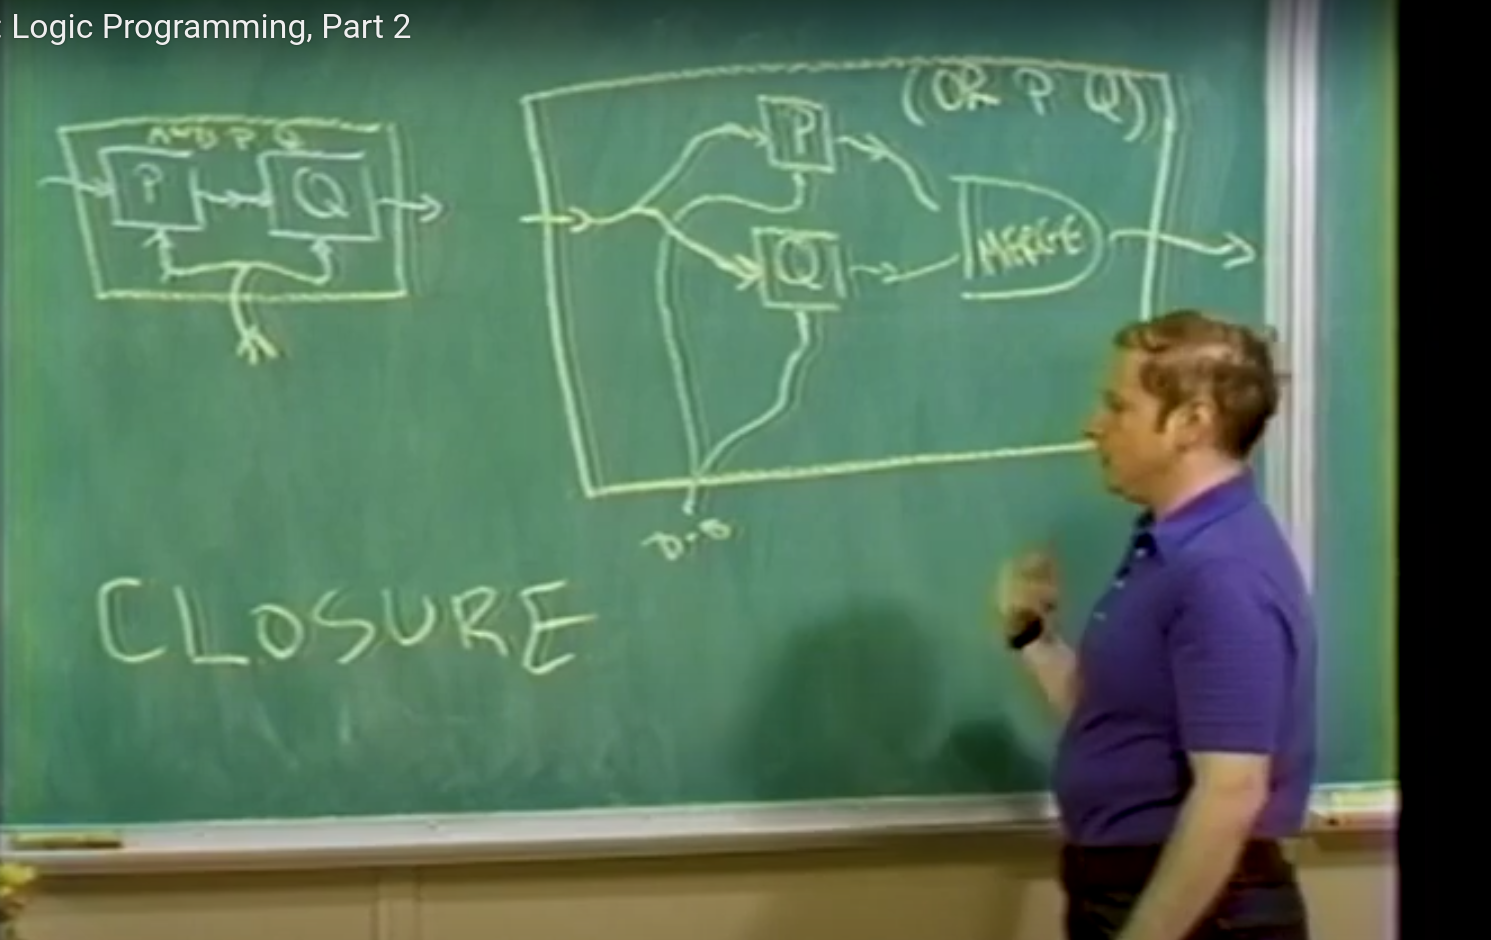
\includegraphics[scale = 0.3]{assets/query_means_combination.png}
\end{center}
AND:
\begin{lstlisting}
+----------------------+
|   +---+      +---+   |
----->| P |----->| Q |------>
|   +---+      +---+   |
|     ^          ^     |
|     |          |     |
|     +-----+----+     |
+-----------|----------+
            |
        database
\end{lstlisting}
AND combination of two queries is produced by operating on the stream of frames in series.\newline
OR
\begin{lstlisting}
    +---------------------------+
    |        +---+      +---+   |
    |  +---->| P |----->| m |   |
    |  |     +---+      | e |   |
  -----+       ^        | r |-------->
    |  |     +---+      | g |   |
       +---->| Q |----->| e |   |
    |        +---+      +---+   |
    |          ^                |
    +----------|----------------+
               |
            database
\end{lstlisting}
OR  combination of two queries is produced by operating on the stream of frames in
parallel and merging the results.

NOT
\begin{lstlisting}
filter
+---+
----->| P |----->
+---+
  ^
  |
\end{lstlisting}
\textbf{Principle of closure: all these elements have the same shape}

\subsection{Means of abstraction - Rules}
A unifier is a slight generalization of the pattern matcher which takes two patterns and finds what are the most general things which can be substitued to satisfy both of the simultaneously.

Simple example:

\begin{lstlisting}
unify (?x ?x)
with  ((a ?y c) (a b ?z))

    ?x : (a b c)
    ?y : b
    ?z : c
\end{lstlisting}
Use unifiers to get more complex pattern matching.

\subsection{Evaluation}
Formal similarity with the Metacircular Evaluator:
\begin{itemize}
    \item To apply a rule: evaluate the rule body relative to an environment formed by unifying the rule conclusion with the given query.
    \item To apply a procedure: evaluate the procedure body relative to an environment formed by binding the procedure parameters with the given arguments.
\end{itemize}

\subsection{Is Logic Programming Mathematical Logic?}
Our query language does not behave like classical predicate logic, our logic operators are not commutative.
Switch the order of statements may trigger an infinite loop.
A and B != B and A
First filters out A then filters out B != First Filter out B then filter out A
If A >> B, then first search would take much more time (can enter infinite loop)

But also bigger problem:
B and (not A) != (not A) and B (deducing from the rules we have)
In logic, we interpret the statement "not P" to mean that P is not true. In the query system, however,
"not P|| means that P is not deducible from the knowledge in the data base.

\section{Lecture 9A: Register Machines}
Goal of this section: demystify the inner parts of the computer - learn how its hardware ware works,
controls the flow of the processes you write in a program
\begin{itemize}
    \item Program is in fact a description of a machine.
    \item Traditional computers also known as register machines sequentially execute instructions
    that manipulate the contents of a fixed set of storage elements called registers.
    \item To design a register machine, we must design its data paths (registers and operations) and
    the controller that sequences these operations.
\end{itemize}

\subsection{Demystification of the Mechanisms of Execution}
\begin{example}
    Les't turn simple Lisp programs into hardware.
\end{example}

\begin{lstlisting}[language=Lisp]
    (define (gcd a b)
        (if (= b 0)
            a
            (gcd b (remainder a b))))
\end{lstlisting}

\begin{definition}
    Register is a place for storing data.
\end{definition}

\begin{definition}
    My computer hardware needs two things \textbf{data paths} - like buttons which need to be
    activated and a \textbf{controller} - decides when to push the different buttons.
\end{definition}

Data path:
\begin{lstlisting}
a                 b                 lightball lights if b == 0
+----------+      +----------+      /-------\
| register |<-----| register |----->| zero? |
+----------+      +----------+      \-------/
          |        |    ^
          V        V    |
        /------------\  |
        | remainder  |  |
        \------------/  |
              |         |
        swap  V         |
         +----------+   |
         | register |---+
         +----------+

\end{lstlisting}
Data path of a GCD machine:
\begin{enumerate}
    \item We can move the content of b to a
    \item We can calculate the remainder of a and b
    \item We can check if b is 0.
    \item We need a temporary storage swap (since all operations happen one at a time)
    \item We can store swap into b
\end{enumerate}

\begin{itemize}
    \item Controller is like a maze connected by a bunch of arrows.
    \item The controller manages or directs the flow of data between two entities.
    \item The thing on the right is controller, on the left is the data path
\end{itemize}

\begin{center}
    \includegraphics[scale = 0.2]{assets/controller.png}
\end{center}
Controller:
\begin{lstlisting}[language=Lisp]
  loop:
  IF b = 0
    DONE
  ELSE
    t <- remainder
    a <- b
    b <- t
    GOTO loop
\end{lstlisting}

We create a language to represent the machine:
\begin{lstlisting}[language = Python]
    def-machine gcd(, controller = loop) -> List[Callable]:
        registers  = a,b,swap
        controller = loop:
                        if we are on branch 0: fetch b -> done
                        assign swap remainder(fetch a, fetch b)
                        assign a to (fetch b)
                        assign b to (fetch swap)
                        go to loop

        return registers, controller
\end{lstlisting}
Add I/O to get input and display output:
\begin{lstlisting}[language = Python]
    def-machine gcd(, controller = loop) -> List[Callable]:
        registers  = a,b,swap
        controller =
                    main:
                    (assign a to (read))
                    (assign b to (read))
                    loop:
                        if we are on branch 0: fetch b -> done
                        assign swap remainder(fetch a, fetch b)
                        assign a to (fetch b)
                        assign b to (fetch swap)
                        go to loop
                    done (perform (print (fetch a))
                    (goto main)
        return registers, controller
\end{lstlisting}
\texttt{read} and \texttt{write} are complicated and be on their own other machines.

\subsection{Build machine language for recursive processes}
\begin{lstlisting}[language = Python]
    def fact(n):
        if n == 1: return 1
        return n*fact(n-1)
\end{lstlisting}
We need to simulate infinite machines- the outer machine needs to know the existence of the inner machine.

Architecture of hardware for iterative machine vs recursive:
Iterative is WITHUOUT a stack.
Recursion is WITH the stack.

\begin{center}
    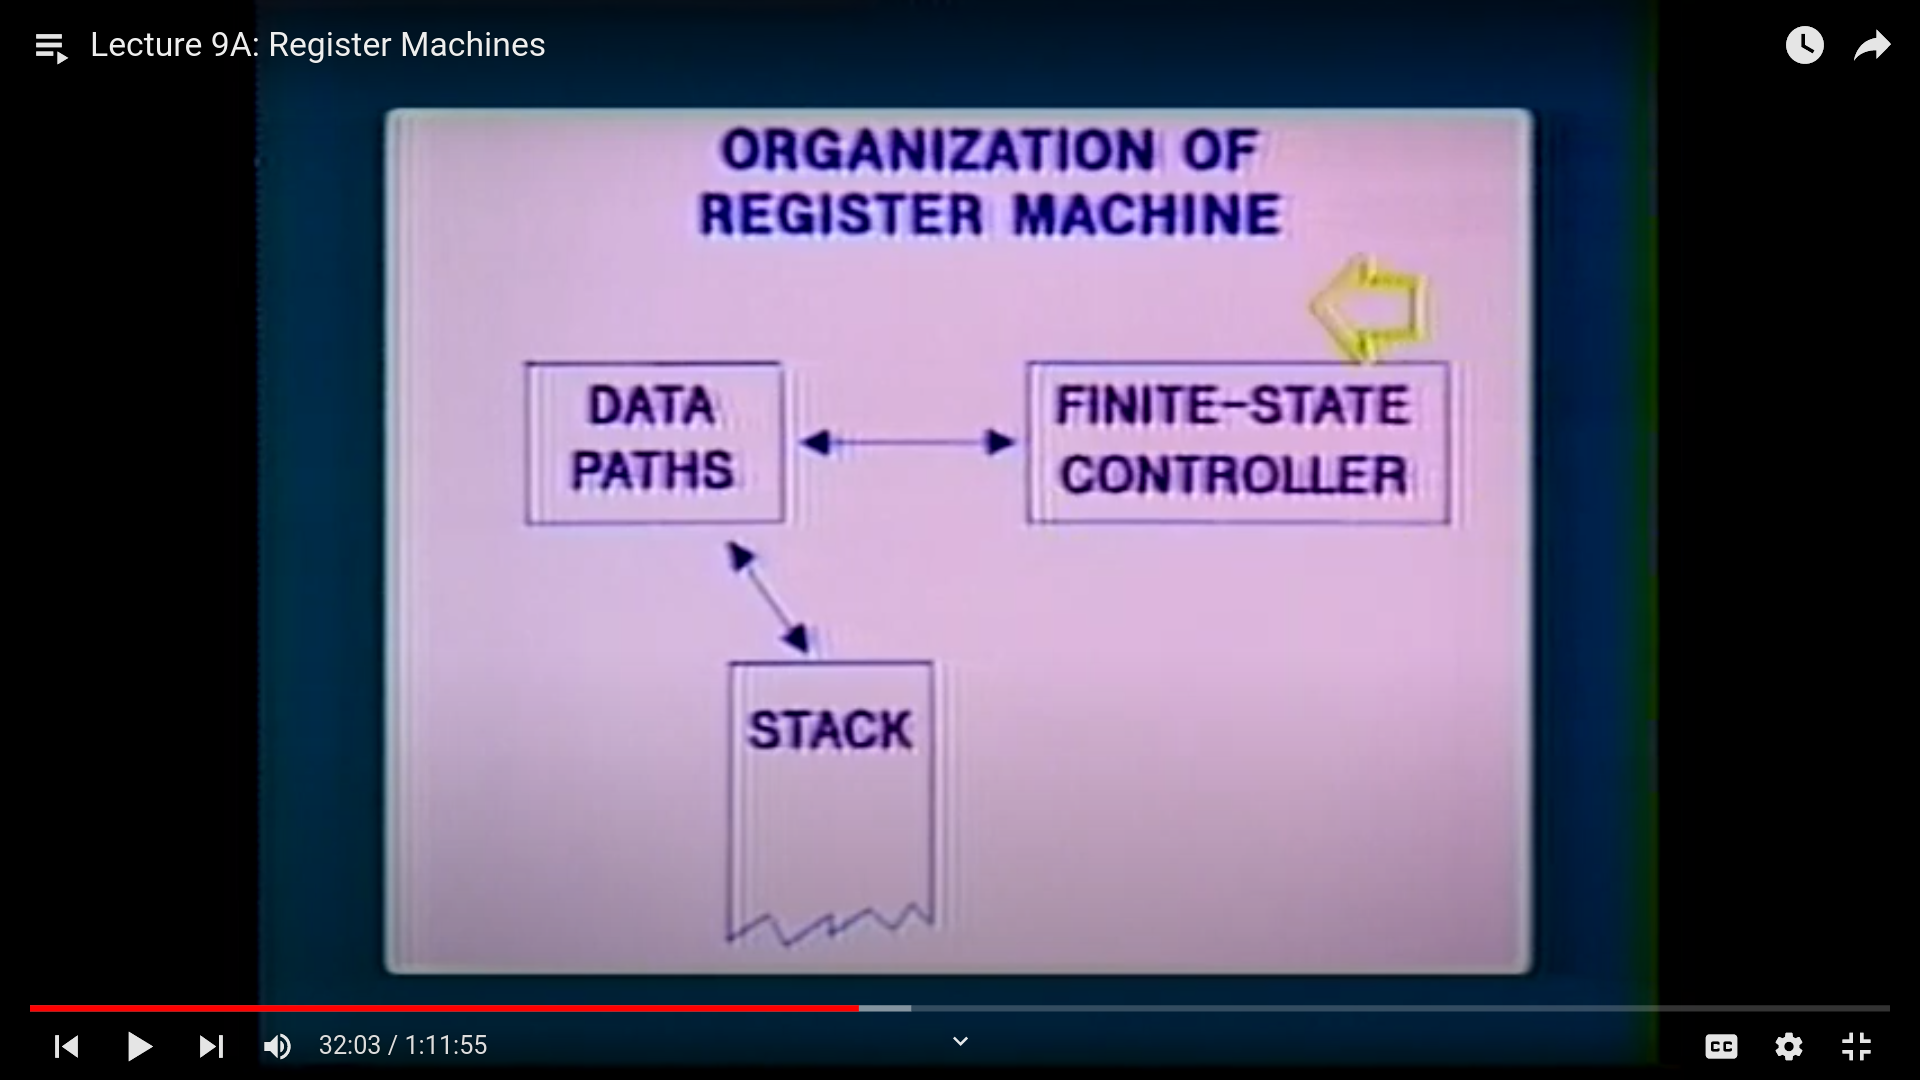
\includegraphics[scale = 0.2]{assets/iterative_machine.png}
\end{center}
We obviously cannot nest an infinite number of machines, we need an "illusion" to make our machine
look as infinite as we need it to be.


\begin{lstlisting}[language = Python]
+------------+        +-------------------------+  \
| data paths |<------>| finite-state controller |   | finite
+------------+        +-------------------------+  /
      ^
      |
      v                                            \
+------------+                                      | "infinite"
|   stack    |                                      |
|            |                                      |  keeps track of the state
.            .                                      |  of the "outer machine"
.            .                                      |
:            :                                      |

\end{lstlisting}
Let's design the machine:
\begin{lstlisting}[language = Python]
                                                        Constants
                                                   +-------+    +------+
                                                   | after |    | done |
                                                   +-------+    +------+
                                                          |       |
                                                          V       V
                                                       /------------\
                                                       | controller |
                                                       \------------/
                         (two way connection)                ^
                          +------------------------+         | continue (connects the controller with the stack)
                          |                        |         |
 val                n     V                        V         V
+----------+      +----------+      /------\     +---------------+
| register |<-----| register |----->| one? |     |    stack      |
+----------+      +----------+      \------/     +---------------+
   ^     |         |      | ^                    |               |
   |     V         V      V |                    +---------------+
   |   /------------\   /-------------\          +---------------+
   +---|  multipler |   | decrementer |          +---------------+
       \------------/   \-------------/          .               .
                                                 :               :
\end{lstlisting}
The above graph shows how the controller is connected to the data paths.
On the right is the controller structure, on the left is the data path.

\section{Lecture 9B: Explicit-control Evaluator}
We have seen the \textbf{magic} of building languages:

\begin{itemize}
    \item Escher Picture language
    \item Digital logic language
    \item Query language
\end{itemize}
All based on Lisp.
\begin{itemize}
    \item  Lisp is not good for solving any particular problem.
    \item  What Lisp is good for is constructing within it the right language to solve the problem you want to solve.
\end{itemize}
What's Lisp based on? Lisp is based on Lisp: cfr the \textbf{metacircular evaluator}.

\begin{center}
    To make the magic disappear: let's implement Lisp in terms of a register machine architecture
\end{center}
\begin{lstlisting}
+-------------------------+     +------------+     +---------- - -  -   -
| finite state controller |<--->| data paths |<--->| stack
+-------------------------+     +------------+     +---------- - -  -   -
\end{lstlisting}

As opposed to the metacircular evaluater having a Lisp evaluator built by a register machine should
make you feel confortable how it works. Last time we saw how the GCD and Fibonacci are translated from Lisp
to the register machine language. What we need to do here is to translate the procedure of the metacircular
evaluator for a register machine.

Models of computation so far:
\begin{center}
    Substitution model --> Environment model --> Metacircular evaluator --> Register machines
\end{center}

Architecture of a Lisp System
\begin{lstlisting}
          characters           ist structure obj
    User ------------> Reader ----------------> Evaluator ----------> Printer
     ^                   | has                     | has                   |
     |                   V                         V                       |
     |             List Structure               Primitive                  |
     |                Memory                    Operators                  |
     |                                                                     |
     +---------------------------------------------------------------------+
\end{lstlisting}
\begin{itemize}
    \item list structure obj = pointers and values
    \item REPL = Read Evaluate Print Loop
\end{itemize}
We will focus on the evaluator (nothing special - just a aparticular register machine),
it has 7 registers:
\begin{enumerate}
    \item exp, expression to to be evaluated (pointer to List Structure Memory)
    \item env, evaluation environment (pointer to List Structure Memory)
    \item fun, procedure to be applied
    \item argl, list of evaluated argument
    \item continue, place to go to next
    \item val, result of evaluation
    \item unev, temporary register for expressions
\end{enumerate}
First four do the \textbf{eval-apply} loop.
\begin{center}
    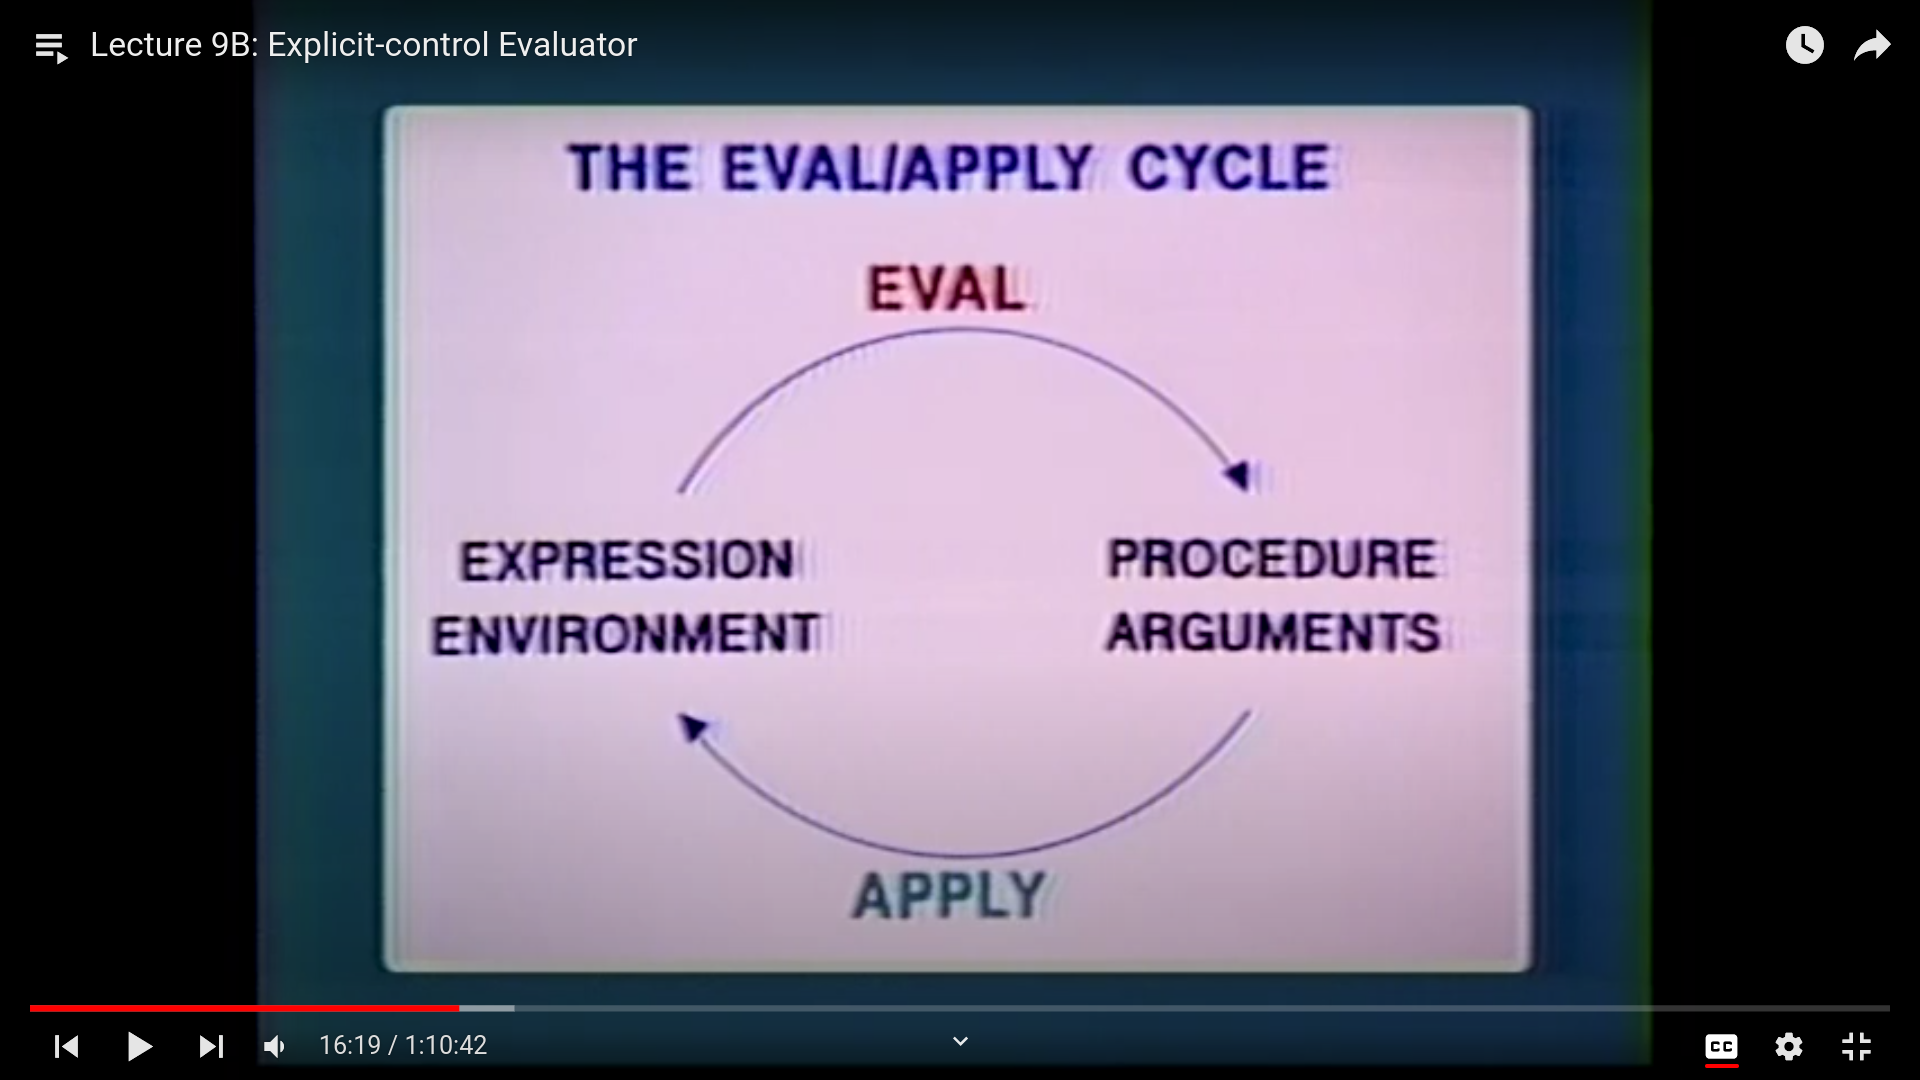
\includegraphics[scale = 0.2]{assets/eval-apply-loop.png}
\end{center}
Two main parts of register machine ofr Lisp are \texttt{eval-dispatch} and \texttt{apply-dispatch}.

Contract that \texttt{eval-dispatch} fulfills:
\begin{itemize}
\item the \texttt{exp} register holds an expression to be evaluated
\item the \texttt{env} register holds the environment in which the expression is to be evaluated
\item the \texttt{continue} register holds a place to go next
\item the result will be left in the \texttt{val} register
\item the contents of all other registers may be destroyed
\end{itemize}

Contract that \texttt{apply-dispatch} fulfills:
\begin{itemize}
\item the \texttt{argl} register contains a list of arguments
\item the \texttt{fun} register contains a procedure to be applied
\item the top of the \texttt{stack} holds a place to go next
\item the result will be left in the \texttt{val} register
\item the \texttt{stack} will be popped
\item the contents of all other registers may be destroyed
\end{itemize}

\subsection{Evaluator (Partial)}
\begin{lstlisting}[language=Lisp]
    eval-dispatch
  (branch (self-evaluating? (fetch exp)) ev-self-eval)
  (branch (variable? (fetch exp)) ev-variable)
  ; ...
  (branch (application? (fetch exp)) ev-application)
  (goto unknown-expression-error)

ev-self-eval
  (assign val (fetch exp))
  (goto (fetch continue))

ev-variable
  (assign val (lookup-variable-value (fetch env)))
  (goto (fetch continue))

ev-application
  (assign unev (operands (fetch exp)))
  (assign exp (operator (fetch exp)))  ; replace the expression by the operation to apply
  (save continue)
  (save env)
  (save unev)
  (assign continue eval-args)
  (goto eval-dispatch)                 ; recursive call

eval-args
  (restore unev)
  (restore env)
  (assign fun (fetch val))
  (save fun)
  (assign argl '())
  (goto eval-arg-loop)

eval-arg-loop
  (save argl)
  (assign exp (first-operand (fetch unev)))
  (branch (last-operand? (fetch unev)) eval-last-arg)
  (save env)
  (save unev)
  (assign continue accumulate-arg)
  (goto eval-dispatch)

accumulate-arg
  (restore unev)
  (restore env)
  (restore argl)
  (assign argl (cons val) (fetch argl))
  (assign unev (rest-operands (fetch unev)))
  (goot eval-arg-loop)

eval-last-arg
  (assign continue accumulate-last-arg)
  (goto eval-dispatch)

accumulate-last-arg
  (restore argl)
  (assign argl (cons (fetch val) (fetch argl)))
  (restore fun)
  (goto apply-dispatch)
\end{lstlisting}


\subsection{Applicator}
\begin{lstlisting}[language=Lisp]
    apply-dispatch
    (branch (primitive-proc? (fetch fun)) primitive-apply)
    (branch (compound-proc? (fetch fun)) compound-apply)
    (goto unknown-proc-type-error)
  
  primitive-apply
    (assign val (apply-primitive-proc (fetch fun) (fetch argl)))
    (restore continue)
    (goto (fetch continue))
  
  compound-apply
    (assign exp (procedure-body (fetch fun)))
    (assign env (make-bindings (fetch fun) (fetch argl)))
    (restore continue)     ; this is where tail recursion happens
    (goto eval-dispatch)
\end{lstlisting}

Assume having an environment with $x=5$ and $y=3$. Evaluating $x+y$  inside the Eval-Apply loop is a
recursive procedure in nature. See \href{https://youtu.be/Z8-qWEEwTCk?list=PLE18841CABEA24090&t=1281}{youtube video}
We need to evaluate the expressions $x$ and $y$ then we need to apply $+$. Recursion appears not only
when computing factorials and fibonacci numbers, the evaluation process in general is recursive and you
use the recursion stack.\newline
\begin{definition}
Applying a procedure results in evaluating the body of the procedure which in turns might result in
applying another procedure.
\end{definition}
\begin{center}
    Aside: Iterative procedure in Lisp has recursive structure = Recursive tail function.
\end{center}

There is no magic in how computers execute code. You can have it in your hand:
\begin{center}
    \includegraphics[scale =0.2]{assets/chip.png}
\end{center}

\section{Lecture 10A: Compilation}
Last time we looked at an \textbf{explicit control evaluator} for Lisp - bridged the gap between
higher level language Lisp and conventional register machine.

We take a lower level language (machine code/assembly) and we're raising the machine to a higher-level
language like Lisp by writing an \textbf{interpreter}.

\subsection{Interpreters}

\begin{lstlisting}
    +-----------------------------------+
    |         Lisp Interpreter          |
    | +-------------------------------+ |
    | | Register Language Interpreter | |
 5  | +-------------------------------+ | 120
---->|         ^                ^        |----->
    | /----------------\  /---------\   |
    | | (assign val    |  | Library |   |
    | |   (fetch exp)) |  \---------/   |
    | \----------------/                |
    +-----------------------------------+
                      ^
            /------------------\
            | (define (fact n) |
            |   (if ...))      |
            \------------------/
\end{lstlisting}
\begin{center}
    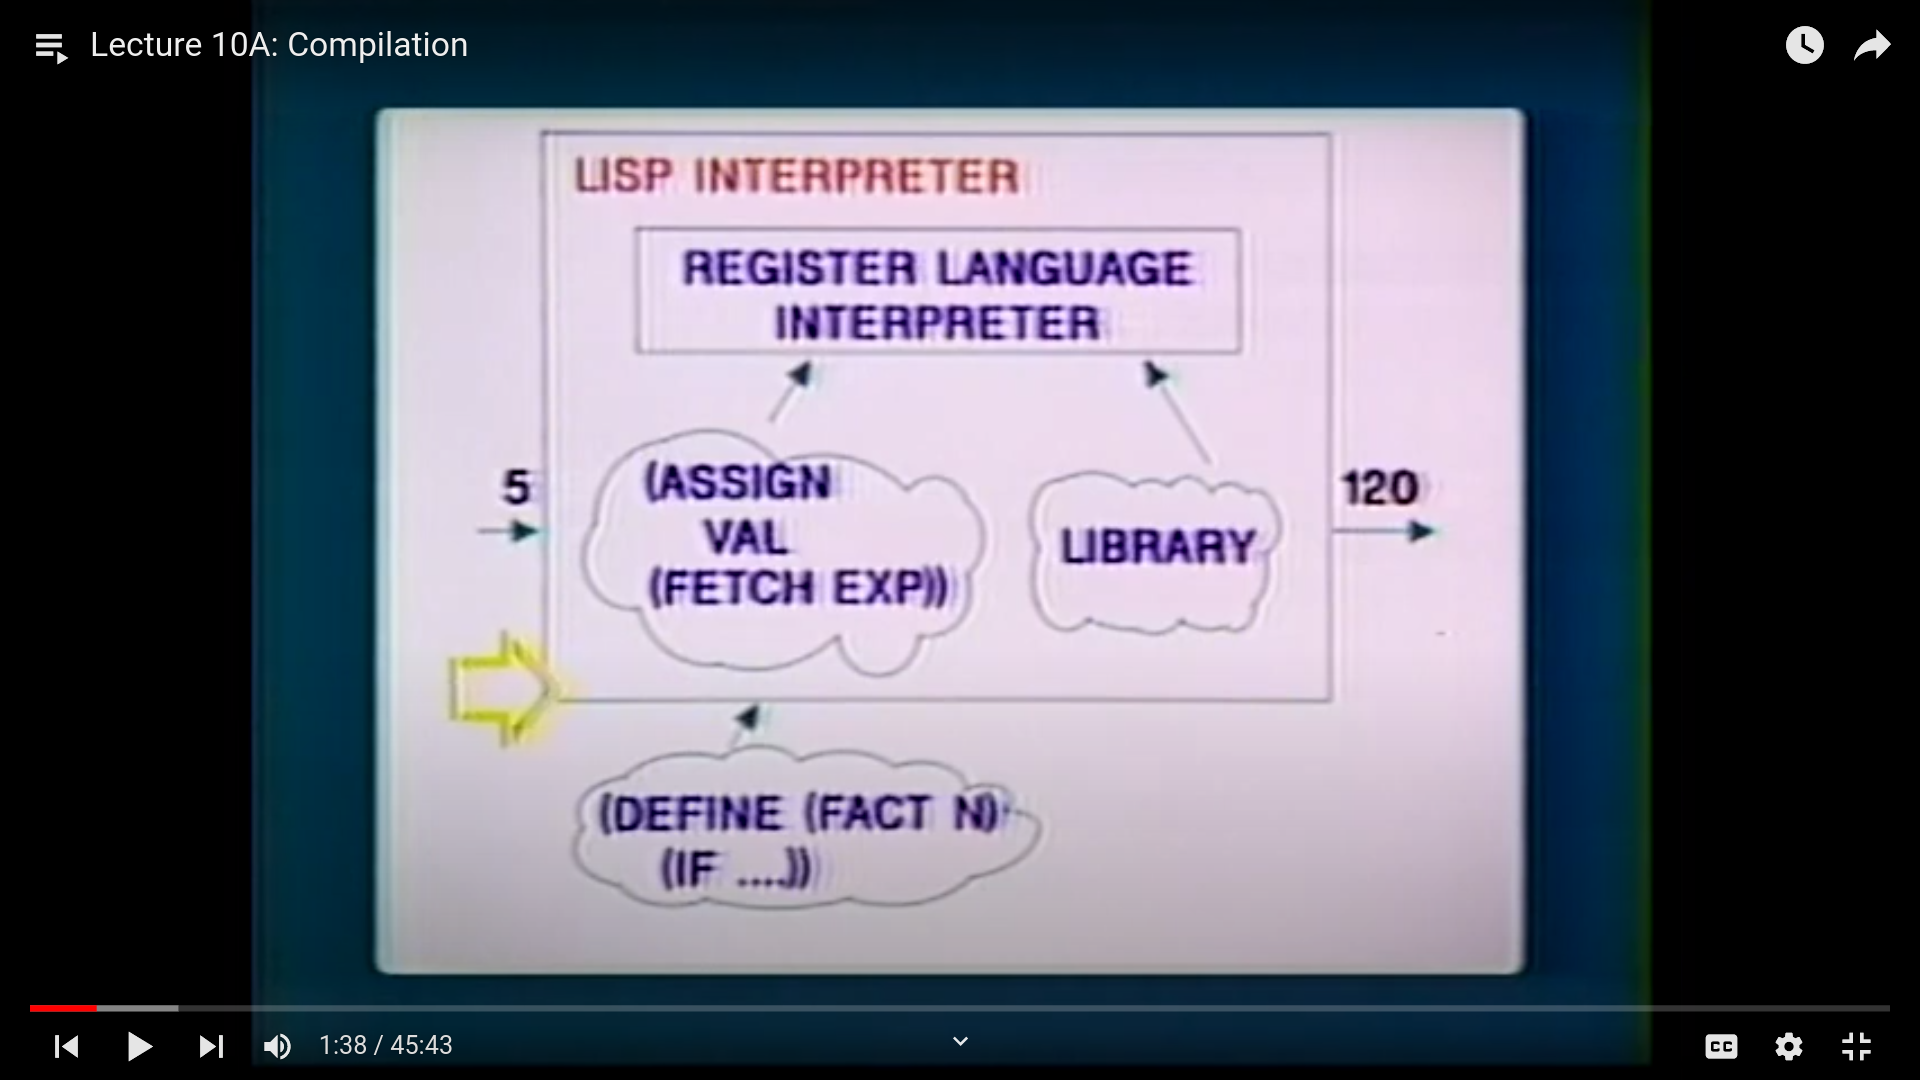
\includegraphics[scale = 0.2]{assets/lisp_interpreter.png}
\end{center}

We are writing an (Lisp) interpreter to raise the machine to the level of the programs we want to write.

\subsection{Compilers}
Compilation is different than interpretation strategy.
\begin{proposition}
    We lower our language down to the level of the machine in order to make our code run more efficiently.
\end{proposition}
\begin{lstlisting}
    /------------------\  source code   +----------+
    | (define (fact n) |--------------->| Compiler |
    |   (if ...))      |                +----------+
    \------------------/                     |   translates into
                                object code  |   register language
                                             |
                                             V
                                /----------------\
               +--------+       | (assign val    |
               |        |<------|   (fetch exp)) |  machine code/assembly
               | Linker |       \----------------/
               |   /
               | Loader |       /---------\
               |        |<------| Library |
               +--------+       \---------/
                   |
                   | load module
                   |
                   V
          +-------------------+
      5   | Register Language | 120
    ----->|    Interpreter    |----->
          +-------------------+

\end{lstlisting}


\begin{center}
    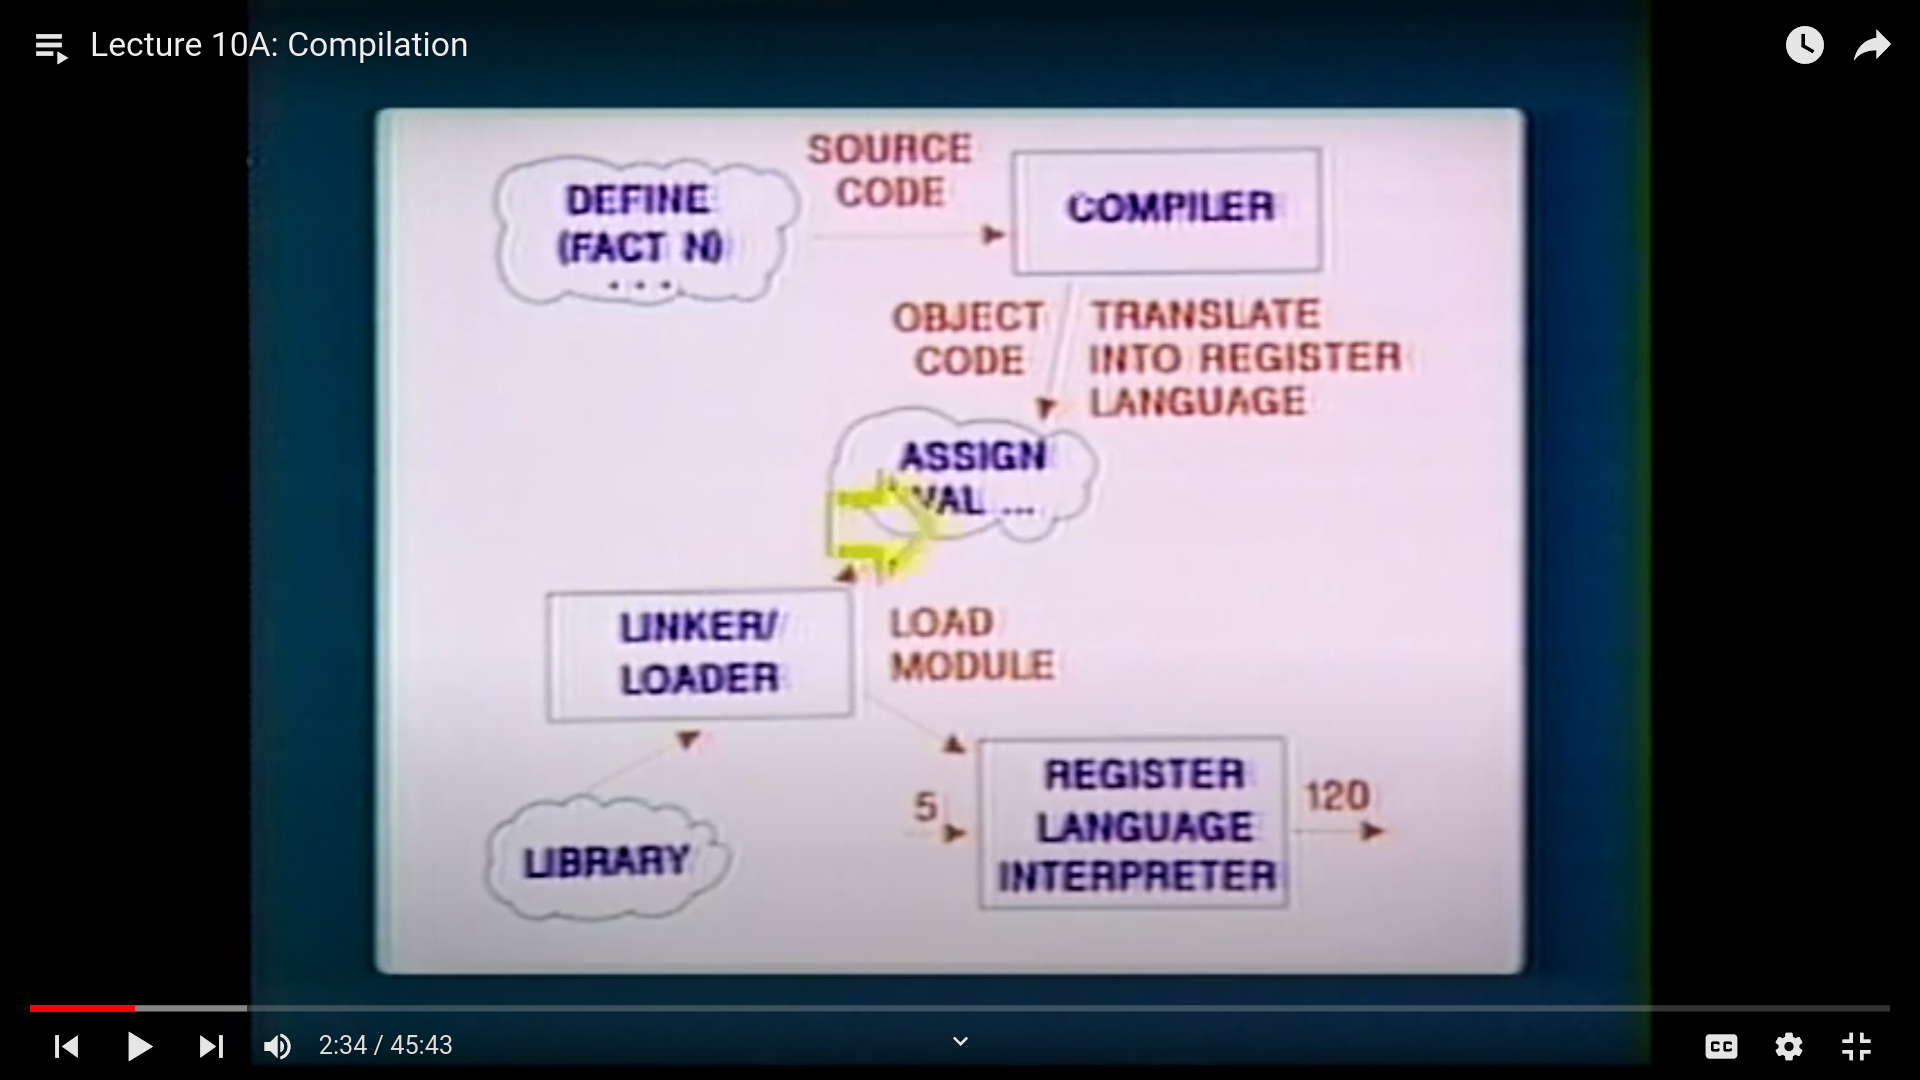
\includegraphics[scale = 0.2]{assets/compilers.png}
\end{center}
Recall register operations are those performed by the controller and the data paths inside your chip.\\
\textbf{Compiler vs Interpreter}
\begin{itemize}
    \item The interpreter has to produce register operations which are general
    enough to run ANY Lisp procedure.
    \item The compiler has to produce register operations which are specific to the particular Lisp
    procedure
    \item The interpreter is a general purpose simulator - read in any Lisp procedure -> translate to
    machine code which performs register operations on the chip
    \item The compiler is configuring to BE the machine that the interpreter would have been simulating.
    \item Compiler produces code which is faster.
    \item Interpreter is better for debugging. You have the library inside the interpreter so you can put
    breakpoints and debug.
    \item Compiled languages have at 2 least steps to get from source code to execution.
    \item Interpreted languages have only one execution.
\end{itemize}

\begin{example}
    To build a very simple compiler, we can simply capture the output of the evaluator instead of interpreting it.\\
    Example: register operations in interpreting $(f x)$
\end{example}

\begin{lstlisting}[language=Lisp]
    (assign unev (operands (fetch exp)))
    (assign exp (operator (fetch exp)))
    (save continue)
    (save env)
    (save unev)
    (assign continue eval-args)
    (assign val (lookup-var-val (fetch exp (fetch env))))
    (restore unev)
    (restore env)
    (assign fun (fetch val))
    (save fun)
    (assign argl '())
    (save argl)
    ...
\end{lstlisting}
Recall \texttt{unev}, \texttt{exp} are registers (placeholders for data).\\
Run Compiler ~ Run the explicit evaluator but stash operations instead of actually executing them. \\
Except when you have conditional statement at compile time since you do not execute anything you do not
know which branch you need to "compile" - so you compile both branches.
\begin{proposition}
    Simple compiler would be just to have the evaluator stashing operations. Here we have already gained
    better performance - if ou run the evaluator 1000 times you need to do the execution of the evaluator 1000
    times which includes evaluating that $(f x)$ is \texttt{eval-application}. Where as in compiled you
    analyze once that it is \texttt{eval-application} and do not do that analysis anymore.
\end{proposition}

\subsection{Optimizations}
In the previous register operations example, some irrelevant operations were emitted because
they deal with constants. The 19 initial operations can be optimized into a sequence of only 10 instructions:

\begin{lstlisting}
    (save env)
    (assign val (lookup-var-val 'f (fetch env)))
    (restore env)
    (assign fun (fetch val))
    (assign arg '())
    (save argl)
    (assign val (lookup-var-val 'x (fetch env)))
    (restore argl)
    (assign argl (cons (fetch val) (fetch argl)))
    (restore fun)
\end{lstlisting}

Interpreter deals with the process of evaluation of a general program. Compiler can work with constants
and has particular operations. Now if we get rid of the useless stack operations, we are down to this:
\begin{lstlisting}
    (assign fun (lookup-var-val 'f (fetch env)))
    (assign val (lookup-var-val 'x (fetch env)))
    (assign argl (cons (fetch val) (fetch argl)))
    
    ;; computation proceeds at apply-dispatch
\end{lstlisting}
The general idea is that the compiler can be better than the interpreter, because the interpreter doesn't
know what it's about to encounter. It is a general purpose simulator and has to be maximally pessimistic in
saving register values to protect itself. the compiler only has to deal with what actually had to be saved.


\begin{itemize}
    \item For the interpreter we had 7 register machine
    \item For the compiler you can get rid of the \texttt{exp} and \texttt{unenv} registers as they
    data structures of the evaluator. Those things are constants in the compiler.
\end{itemize}

\subsection{Compiler general strategy}
Assume we want to compile $OP(A_1,A_2)$.
\begin{center}
    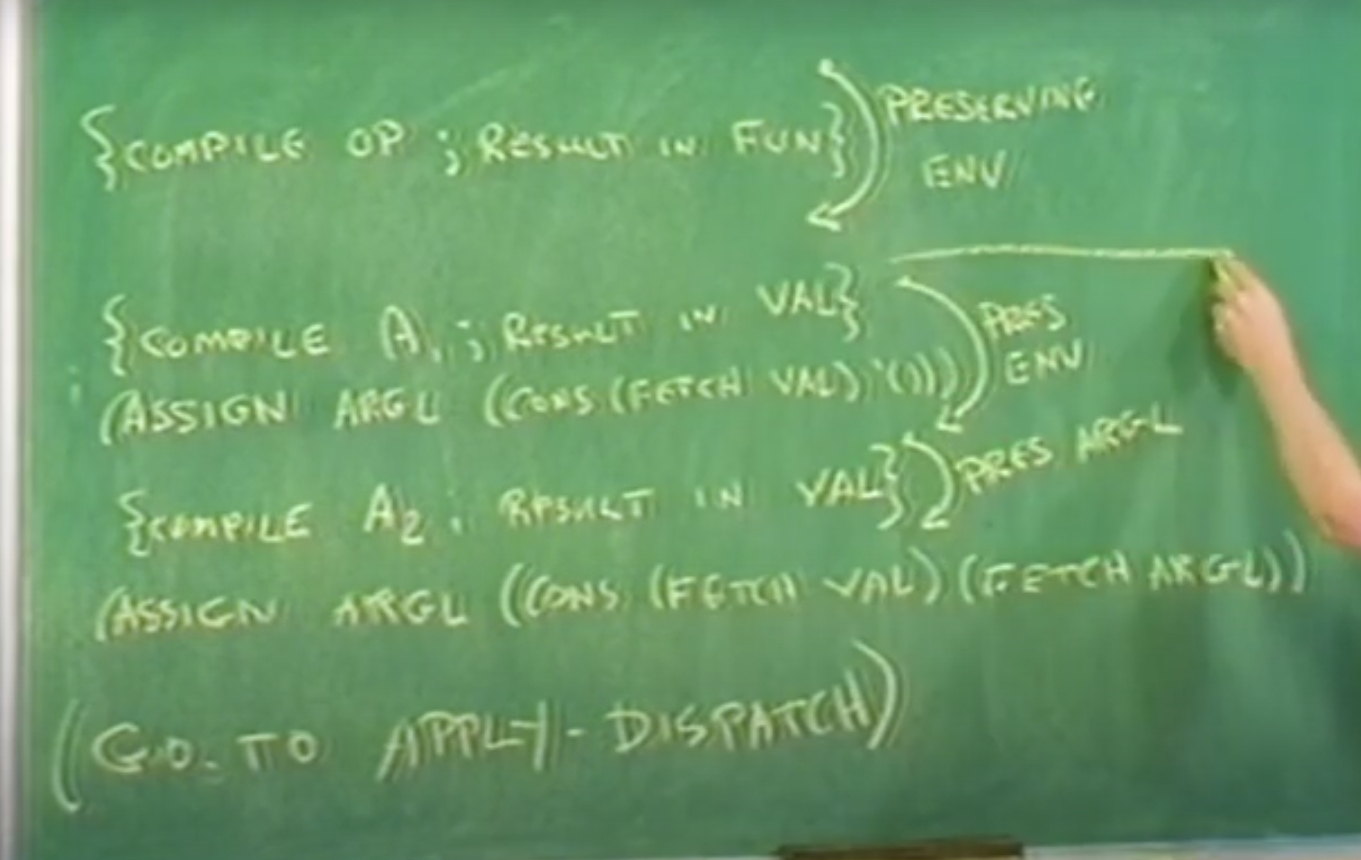
\includegraphics[scale = 0.2]{assets/append_seq_compiler.png}
\end{center}
What the compiler does is to append a bunch of code sequences. If \texttt{seq2} needs \texttt{reg} and \texttt{seq1}
modifies \texttt{reg}:
\begin{lstlisting}
    (save reg)
    <compile seq1>
    (restore reg)
    <compile seq2>
    else
    <compile seq1>
    <compile seq2>
\end{lstlisting}
Where the compiler has the preserving notes, the interpreter is more pessimistic and always saves the state.
To the compiler an annotated code sequence contains:
\begin{itemize}
    \item a sequence of instructions
    \item set of registers modified
    \item set of registers needed
\end{itemize}
Code sequence data structure for the compiler has the above three points.
\begin{example}
    Code sequence for assignement operations $R1 = R2$
\end{example}
\begin{itemize}
    \item a sequence of instructions = (assign r1 (fetch r2))
    \item set of registers modified = {r1}
    \item set of registers needed = {r2}
\end{itemize}
\textbf{Register optimizations} are based what registers are needed and modifier by code fragments.

\section{Lecture 10B: Storage Allocation and Garbage Collection}
How is data represented in computers? When we construct an objet using \texttt{cons} how is that
stored in the computer? We saw that this is equivalent to procedures but still where are procedures set
inside the machine.

\begin{center}
    Memory, the glue that data structures are made of.
\end{center}
Gödel came up with a scheme to encode expressions as numbers.

If objects ar represented by numbers then:
\begin{itemize}
    \item \texttt{(cons x y) }could be represented as $2^x 3^y$
    \item \texttt{ (car x)} could be represented as the number of factors of $2$ in $x$
    \item \texttt{(cdr x)} could be represented as the number of factors of $3$ in $x$
\end{itemize}
This is not very practical. On the other hand, we have been thinking about \texttt{cons} as
\textbf{boxes} with values and pointers. Semiconductor companies do not exactly supply me with that.
They give me \textbf{linear memory} a big pile (array) indexed with addresses.

\subsection{Data Structure Representation}
Our data structures are hierarchical but memory is linear.
\begin{center}
    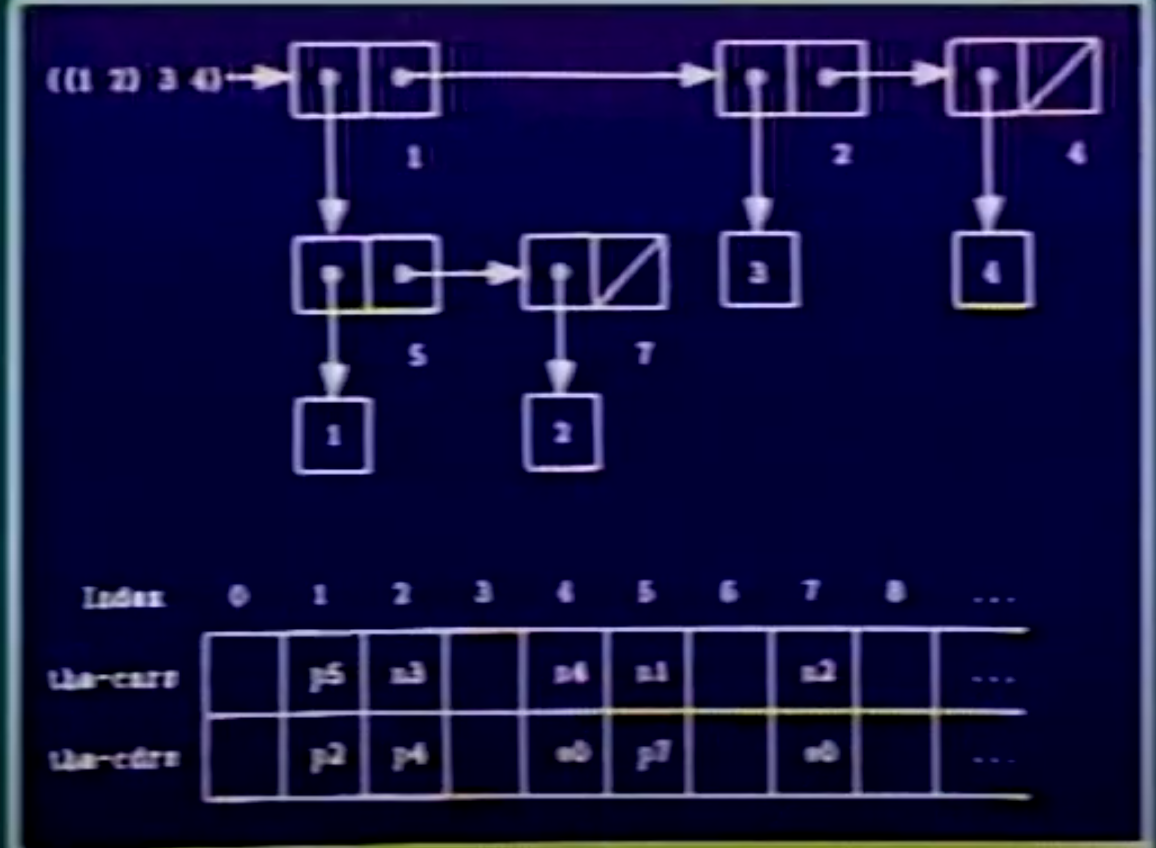
\includegraphics[scale = 0.2]{assets/memory_array.png}
\end{center}

The boxes we have for \texttt{car} and \texttt{cdr} are:
\begin{lstlisting}
    +-+-+                           +-+-+           +-+-+
    ((1 2) 3 4) -> |.|.|-------------------------->|.|.|---------->|.|/|
                   +-+-+                           +-+-+           +-+-+
                    | 1 (*)                         | 2             | 4
                    V                               V               V
                   +-+-+           +-+-+           +-+             +-+
                   |.|.|---------->|.|/|           |3|             |4|
                   +-+-+           +-+-+           +-+             +-+
                    | 5             | 7
                    V               V
                   +-+             +-+
                   |1|             |2|
                   +-+             +-+
    
                   (*) indicates the index in memory
\end{lstlisting}
We divide the memory into two arrays: the-\texttt{cars} and the-\texttt{cdrs}.
These arrays store typed objects, for instance pX is a pair, nX is a number, eX is an empty list, ...
\begin{lstlisting}
    +----------+----+----+----+----+----+----+----+----+----+----
    | Index    |  0 |  1 |  2 |  3 |  4 |  5 |  6 |  7 |  8 | ...
    |----------+----+----+----+----+----+----+----+----+----+----
    | the-cars |    | p5 | n3 |    | n4 | n1 |    | n2 |    |
    |----------+----+----+----+----+----+----+----+----+----+----
    | the-cdrs |    | p2 | e0 |    | e0 | p7 |    | e0 |    |
    +----------+----+----+----+----+----+----+----+----+----+----
\end{lstlisting}
The box notation is just a drawing for us to interpret easily. What really happens inside the computer
is in the gigantic array which is a linear memory. Having pairs within pairs has a binary tree structure.
Given this binary tree you represent it in 2 arrays in memory. \\
Machine code instructions like \texttt{assign} and \texttt{fetch} actually access these arrays.
\begin{lstlisting}
    ;; Accessors
    (vector-ref  vector index)
    (vector-set! vector index value)
    
    (assign a (car (fetch b)))
    ====>
    (assign a (vector-ref (fetch the-cars) (fetch b)))
    
    (assign a (cdr (fetch b)))
    ====>
    (assign a (vector-ref (fetch the-cdrs) (fetch b)))
    
    (perform (set-car! (fetch a) (fetch b)))
    ====>
    (perform (vector-set! (fetch the-cars) (fetch a) (fetch b)))
    
    (perform (set-cdr! (fetch a) (fetch b)))
    ====>
    (perform (vector-set! (fetch the-cdrs) (fetch a) (fetch b)))
\end{lstlisting}

\subsection{Allocation}
How to find free memory and put value in it?
Freelist allocation scheme: all free cells are linked to the next free cell.
\begin{lstlisting}
    free -> f6 -> f8 -> f3 -> f0 -> f9 -> ...
\end{lstlisting}
This would work if you'd have infinite memory...

\subsection{Garbage Collection}
In general we want to have the illusion of infinity (for memory). All we need to do is to
arrange it so that whenever you look, the thing is there.\\
Garbage can be created by program and by user too. The interpretation of programs produces garbage
(e.g. short lived frames during procedure evaluation), users produce garbage too.
\begin{definition}
    Garbage is any object which we can never be reached from your program. Think when you create a
    reference variable and if you delete that reference (or move the reference to point at another object)
    then the initial object is unreachable = garbage.
\end{definition}
How to prove that a given data object will never be used again and that it can be discarded without
affecting any other computations?\\
The registers contain pointers to objects in the Lisp Structured Memory. If any object cannot be
reached by walking through the data structure referenced by any of the registers, its memory can be
reclaimed. The mother board of you computer have:
\begin{itemize}
    \item CPU = Data Path Registers + Finite State Controller
    \item RAM = memory
\end{itemize}
Finite State Controller point at the data paths to control them (push buttons).
The Data path registers point at memory to collect data from there.

\begin{proposition}
    We must find a way to reclaim that garbage.
\end{proposition}



\subsubsection{Mark and Sweep Strategy}
For each of the machine registers, we recursively crawl the data structure they reference and mark
the memory cells as we access them. Once this process is completed, all the unmarked cells can be recycled.
\begin{example}
    Example.
\end{example}
\begin{lstlisting}
    root (*)
    |
    V
+-----------+----+----+----+----+----+----+----+----+----
| Index     |  0 |  1 |  2 |  3 |  4 |  5 |  6 |  7 | ...
|-----------+----+----+----+----+----+----+----+----+----
| the-cars  | p3 | p5 | n3 | p0 | p7 | n1 | n4 | n2 |
|-----------+----+----+----+----+----+----+----+----+----
| the-cdrs  | p2 | p2 | p4 | p6 | e0 | p7 | n2 | e0 |
|-----------+----+----+----+----+----+----+----+----+----
| the-marks |  0 |  0 |  0 |  0 |  0 |  0 |  0 |  0 |
+-----------+----+----+----+----+----+----+----+----+----

(*) arbitrarily chosen, could be multiple (all registers)
\end{lstlisting}
We walk the structure, depth-first:
\begin{lstlisting}
    1 -> 5 -> 7
    -> 2 -> 4 (-> 7)
\end{lstlisting}
After the marking process:
\begin{lstlisting}
    +-----------+----+----+----+----+----+----+----+----+----
    | Index     |  0 |  1 |  2 |  3 |  4 |  5 |  6 |  7 | ...
    |-----------+----+----+----+----+----+----+----+----+----
    | the-cars  | p3 | p5 | n3 | p0 | p7 | n1 | n4 | n2 |
    |-----------+----+----+----+----+----+----+----+----+----
    | the-cdrs  | p2 | p2 | p4 | p6 | e0 | p7 | n2 | e0 |
    |-----------+----+----+----+----+----+----+----+----+----
    | the-marks |  0 |  1 |  1 |  0 |  1 |  1 |  0 |  1 |
    +-----------+----+----+----+----+----+----+----+----+----
\end{lstlisting}
When we activate the GC we need to scan the whole memory. Inefficient.

\subsubsection{Minsky-Fenichel-Yochelson Algorithm}
This is known as a \textbf{stop and copy} algorithm. Probably the fastest one for GC so far.
Pre-requisite: we have about twice as much address space as we're using.
We start with a mixture of useful data and garbage and we will gradually copy the good stuff into another space.
\begin{center}
    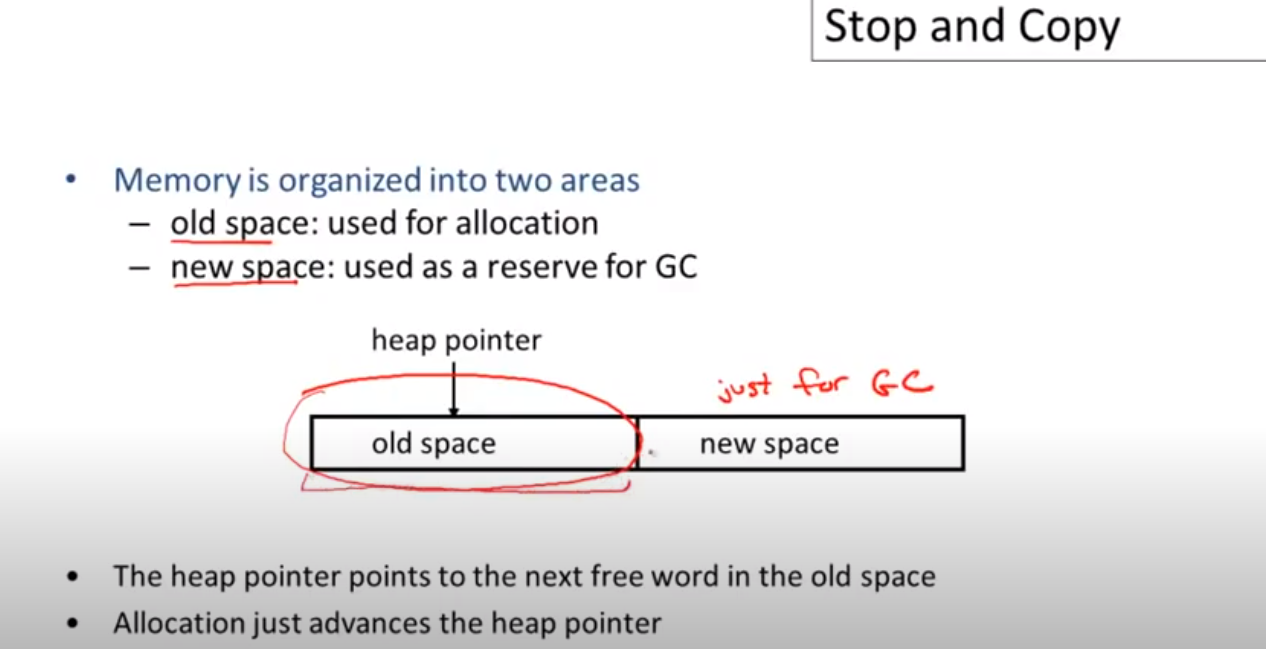
\includegraphics[scale = 0.3]{assets/stop_copy_strategy.png}
\end{center}
\begin{center}
    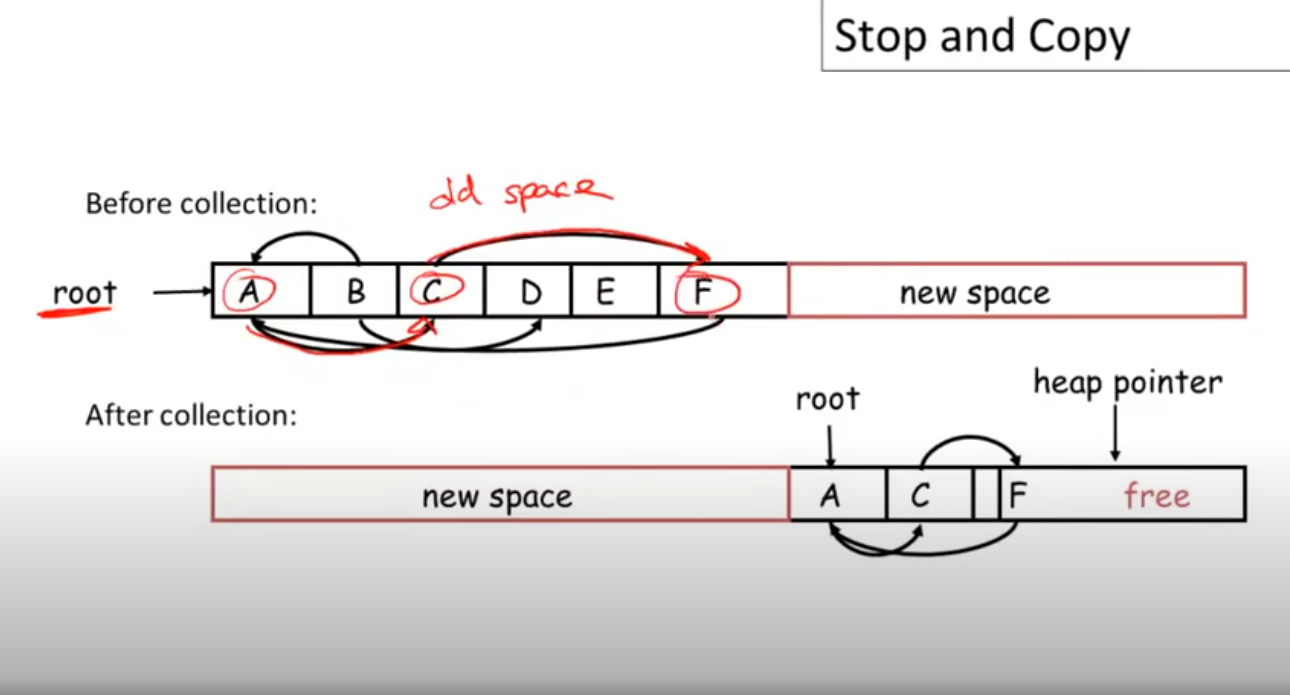
\includegraphics[scale = 0.3]{assets/stop_copy.png}
\end{center}
The old space is called the \textbf{heap} (in JAVA too!).
Java objects reside in an area called the heap. The heap is created when the JVM starts up and may
increase or decrease in size while the application runs. When the heap becomes full, garbage is collected.
During the garbage collection objects that are no longer used are cleared, thus making space for new objects.
\begin{itemize}
    \item Allocation is very cheep just move the pointer.
    \item Collection is relatively cheap - touch only live objects (do not need to touch garbage unlike mark and sweep algo).
\end{itemize}


\subsection{Not Everything Can Be Computed - Halting Theorem}
We want a program which checks if other programs finish in finite time.
Let's imagine a mathematical function $S$ which takes a procedure and its arguments as variables:
\begin{lstlisting}
    S[P, a] = true  if (P a) will converge to a value without an error
    false if (P a) loops forever or makes an error
\end{lstlisting}
Can we write such procedure $S$ that computes the value of $S$?
\subsection{Proof by contradiction}
Suppose we have procedure $is_safe$ that computes the value of $S$.
\begin{lstlisting}
    def is_safe_diag1(arg):
        if is_safe(diag1,arg):
            return infinite_loop_func()
        else:
            return "Not Safe"

    def g():
        if halts(g): # halts(g) must either return true or false by assumption
            loop_forever()

\end{lstlisting}
Computing $is_safe_diag1(diag1)$ shows that $is_safe$ function does not work.
If it's safe ot run diag1 then it will go into an infinite loop which makes it, by definition, unsafe.
We have proved the \href{https://en.wikipedia.org/wiki/Halting_problem}{Halting problem}.

\end{document}
